\chapter*{Modulação deleuzeana, modulação algorítmica e~manipulação midiática}

\addcontentsline{toc}{chapter}{Modulação deleuzeana, modulação algorítmica e~manipulação midiática, \scriptsize{por João Francisco Cassino}}

\begin{flushright}
\emph{João Francisco Cassino\footnote{Mestrando em Ciências Humanas e Sociais (\textsc{ufabc}), especialista em Relações Internacionais (\textsc{u}n\textsc{b}), \textsc{mba} em Gestão Empresarial (\textsc{fgv-rj}) e graduado em Jornalismo (Cásper Líbero). Funcionário de carreira da \textsc{bb} Tecnologia e Serviços (Conglomerado Banco do Brasil).}}
\end{flushright}

\epigraph{Quem controla o passado, controla o futuro. Quem controla o presente, controla o passado.}{\textsc{george orwell}, \emph{1984}}

\epigraph{Já deixamos a era da disciplina para entrar no tempo do controle.}{\textsc{maurizio lazzarato}, \emph{As Revoluções do Capitalismo}}

Qual é a diferença entre os conceitos de \emph{manipulação} e de
\emph{modulação}? Este texto tem por objetivo propor uma visão de que os
dois termos, apesar de muito próximos, são diferentes e não devem ser
utilizados para definir as mesmas coisas. Mais do que isso, sugere
diferenciar \emph{modulação} em duas partes: a clássica \emph{modulação
deleuzeana} e a \emph{modulação algorítmica}. Como forma de exemplificar
esta proposição serão utilizados casos das mídias tradicional,
eletrônica e digital e também do \emph{marketing} corporativo. Como
contexto histórico, mostrar"-se"-á a transição da \emph{sociedade
disciplinar}, nascida nos séculos \textsc{xviii} e \textsc{xix}, para a \emph{sociedade de
controle}, típica do final do século \textsc{xx} e deste início do século \textsc{xxi},
que surge com as tecnologias de comunicação em massa e, mais
recentemente, com o advento e popularização das tecnologias digitais em
rede. O gráfico 1 mostra o fluxo de pensamento a ser desenvolvido nesta
abordagem.

%\begin{figure}%[!ht]
%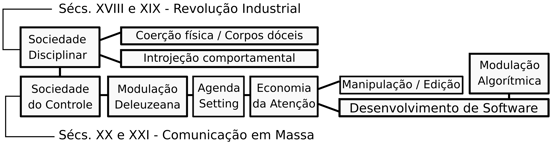
\includegraphics[width=90mm]{./imgs/grafico1.png}
%\caption{\textsc{gráfico} 1 -- Fluxo de Desenvolvimento Teórico.}
%\end{figure}

\section{Sociedade Disciplinar e Sociedade do Controle}

Decorrente do pensamento de Michel Foucault (1989), a \emph{sociedade
disciplinar} se caracteriza quando, com a função de \emph{docilizar
comportamentos,} o poder passa a ser aplicado sobre os corpos dos
indivíduos, inclusive pela \emph{coerção física}. A instrumentalização
das disciplinas precisa da existência de instituições disciplinares,
todas criadas, da forma mais ou menos como as conhecemos hoje, em meados
do século \textsc{xviii}, para suprir as necessidades que surgem com a Revolução
Industrial, com o êxodo do rural para o urbano e com a aparição do
operário fabril. São dessa mesma época as escolas, os hospitais, as
casas de loucos (manicômios) e a prisão pan"-óptica de Jeremy Benthan --
instituições que teriam por função docilizar e vigiar as pessoas
adequando"-as às necessidades do novo modelo capitalista emergente. Aqui
há sempre uma autoridade presente, que ensina, comanda e diz o que
fazer: o professor, o médico, o psiquiatra, o carcereiro. As
instituições feitas para disciplinar os seres humanos têm por derradeiro
objetivo \emph{introjetar o comportamento} dentro de cada pessoa,
criando hábitos, impondo uma cultura que, mesmo na ausência da
vigilância da autoridade, garanta que o agir e o pensar sigam as normas
previamente ditadas.

Já a \emph{sociedade de controle}, como explica Lazzarato:

\begin{quote}
exerce seu poder graças às tecnologias de ação a distância da imagem, do
som e das informações, que funcionam como máquinas de modular e
cristalizar as ondas, as vibrações eletromagnéticas (rádio, televisão),
ou máquinas de modular e cristalizar pacotes de bits (\ldots{}) (2006, p. 85).
\end{quote}

A \emph{modulação}, portanto, tem por poder modular, cristalizar, uma
determinada subjetividade desejada na memória, no cérebro das pessoas.

\begin{quote}
Se as disciplinas moldavam os corpos ao constituir hábitos,
principalmente na memória corporal, as sociedades de controle modulam os
cérebros, constituindo hábitos sobretudo na memória mental
(\textsc{lazzarato}, 2006, p. 86).
\end{quote}

Em síntese, a \emph{sociedade disciplinar} precisa da ação da autoridade
sobre os corpos, até mesmo da punição física, para a introjeção
comportamental. Já a \emph{sociedade de controle} é mais sutil, ocorre à
distância, penetrando os cérebros e forjando as mentes com seus
mecanismos de influência. Portando, o conceito de \emph{modulação},
criado pelo filósofo francês Gilles Deleuze e amplamente utilizado pelo
sociólogo Maurizio Lazzarato, é a base da \emph{sociedade de controle}.

Manuel Castells (2017, p. 209) explica como funcionam os mecanismos de
enquadramento da mente. Para ele, o processamento de informações que
relacionam o conteúdo e o formato da mensagem com molduras
(\emph{frames}) são ativados por mensagens geradas na esfera da
comunicação. O poder de quem gera essas informações, no entanto, é
limitado por como as pessoas selecionam e interpretam essas informações.
Citando a pesquisa \emph{Pew Global Attitudes Project}, Castells
ressalta que somente cerca de 7\% das matérias publicadas na mídia nos
Estados Unidos da América despertaram muita atenção dos telespectadores,
a maioria delas é relativa à segurança ou às violações de normas
sociais. ``O ódio, a ansiedade, o medo e o grande entusiasmo são
particularmente estimulantes e também são retidos na memória de longo
prazo'' (\textsc{castells}, 2017, p. 209), escreve. Quando mecanismos emocionais
são estimulados, o cérebro ativa a capacidade de decisão de nível
superior, buscando e dando mais atenção às informações que recebe. É por
isso que o enquadramento (\emph{framing}) é baseado na provocação de
emoções (\emph{ibid.}, p. 210). Como consequência, o jornalismo abusa do
sensacionalismo e o \emph{marketing} procura atingir os sentimentos dos
consumidores. Inclua"-se na lista de Castells o elemento da erotização,
fortemente presente nos conteúdos midiáticos.

\section{Agenda Setting e Economia da Atenção}

Para o enquadramento de mentes, uma das formas mais poderosas de
influência da mídia sobre seus consumidores é a técnica chamada de
Agenda \emph{Setting}. Como explica o professor Clóvis de Barros Filho
(1996, p. 28), o termo refere"-se à hipótese na qual a agenda temática
dos meios de comunicação impõe os temas de discussão social. Se a mídia
tradicional veicula matérias sobre a Copa do Mundo de Futebol, por
exemplo, espera"-se que a sociedade, nos escritórios, nas salas de aulas
e nos bares, debatam também sobre a Copa do Mundo. Se o agendamento
temático é a violência do tráfico de drogas, esta vira a pauta dos
corredores, dos cafezinhos e nos trens. Clóvis de Barros lembra o
\emph{slogan} de uma extinta emissora de \textsc{tv}: \emph{``Aconteceu Virou
Manchete''}. Logo, presume"-se que se não virou manchete, não aconteceu.
A mesma lógica pode se aplicar ao \emph{slogan} \emph{``Globo e você,
tudo a ver''}. Há aqui um duplo sentindo: pode significar conexão total
com o telespectador, mas também que tudo o que há para se ver, para se
assistir, está na Globo (pelo menos o que há de relevante).

\begin{quote}
Esta construção da realidade social operada pelos meios, por
intermédio de uma seleção e uma hierarquização arbitrária de eventos,
produz efeitos: promove discussões sociais encapsuladas pela barreira do
desconhecimento dos temas jogados no lixo das reuniões de pauta dos
jornais, ou dos que nem chegaram a ela (\textsc{barros}, 1996, p. 28).
\end{quote}

Os editores escolhem quais assuntos serão revelados ao público e quais
serão completamente e deliberadamente ignorados, geralmente sob a
desculpa de falta de tempo (na \textsc{tv} e no rádio) ou de falta de espaço em
páginas impressas (em jornais e revistas). Mas os temas que são de
interesse comercial ou político das emissoras ganham horas e horas e
horas dedicadas na programação.

A \emph{modulação} deleuzeana, base da \emph{sociedade de controle}, que
disputa os espaços nos cérebros das pessoas, usando para tal técnicas de
enquadramento emocional (\emph{framing}) e de imposição de temas na
agenda de debates da vida cotidiana da sociedade (\emph{Agenda Setting})
é tanto um recurso de poder político, social e ideológico quanto um
modelo de negócios altamente lucrativo que sustenta o enorme
conglomerado de mídia mundial.

Em 1971, Herbert A. Simon afirmou que em um mundo repleto de
informações, surge um novo tipo de escassez: a atenção do consumidor.
``Portanto, uma grande quantidade de informações cria uma pobreza de
atenção e uma necessidade de alocar essa atenção eficientemente entre a
superabundância de fontes de informação que poderiam consumi"-la'',
escreve no texto \emph{Designing Organizations for an Information"-rich
World} (p. 40-41). Tal pensamento estimularia que vários pensadores,
tais como Thomas H. Davenport e John C. Beck, passassem a utilizar o
termo ``Economia da Atenção'' para propagar como as organizações
empresariais podem se beneficiar do que eles chamam de uma ``nova moeda
para os negócios''. Entendem que os mercados hoje são ``motores movidos
pelo combustível da atenção''. A atenção é atualmente para as empresas o
que as fazendas e os campos foram para as sociedades rurais, o que as
fábricas foram para a Revolução Industrial e o que o conhecimento é para
a Era da Informação.

\begin{quote}
Mas agora, como os fluxos de informações desnecessárias entopem os
cérebros dos trabalhadores e das comunicações corporativas, a atenção é
um recurso raro que verdadeiramente dá poder a uma empresa (\textsc{davenport};
\textsc{beck}, 2001, p. 17).
\end{quote}

Dizem ainda que a atenção é um recurso valioso que precisa ser
gerenciado como qualquer outro recurso precioso. Uma prova são as
pesquisas chamadas \emph{Top of Mind}, realizadas anualmente, que no
\emph{marketing} empresarial são usadas para qualificar quais são as
marcas mais populares nas mentes dos consumidores. Por meio de
entrevistas, pergunta"-se qual é o nome do primeiro sabão em pó que lhe
vem à cabeça, do primeiro refrigerante, do primeiro tênis, da primeira
marca de produtos eletrônicos e assim por diante. Com isso, mede"-se a
eficiência e a eficácia de uma campanha de publicidade. As marcas mais
lembradas, mais cristalizadas nos cérebros, são as vencedoras desta
competição empresarial. No Brasil, a pesquisa é realizada anualmente
pelo Instituto DataFolha e resulta no prêmio Folha Top of Mind. Em 2017,
as marcas campeãs foram, pela ordem, Omo (com 7\% de menções), Coca"-Cola
(4\%), Nike (4\%) e Samsung (4\%).

Por definição, a gestão de \emph{marketing} tem por um de seus
objetivos:

\begin{quote}
criar ou identificar valor, produzindo inovações estratégicas em
produtos, processos e modelagem de negócios, a partir de um profundo
conhecimento do perfil e das demandas dos mais diferentes públicos e
mercados (\textsc{lima, m}.; \emph{et al}., 2007, p. 19, \emph{apud} \textsc{branstad} e \textsc{lucier}, 2001).
\end{quote}

Essa descrição vai ao encontro do que destaca Lazzarato (2006, p. 101),
de que o \emph{Marketing} tem como uma de suas funções ser capaz de
\emph{criar mundos} como uma das forças de agenciamento de expressão.
Mais do que isso, o \emph{marketing} seria o centro estratégico das
empresas, pois a prática mercadológica seria a de reduzir as
possibilidades das criações e das escolhas, com foco em forçar as opções
sob o jugo de decisões pré"-definidas pelas corporações. Tais opções são
limitadas, mas se mostram como liberdade de escolha aos compradores, mas
a liberdade de escolher se resume ao que as empresas ofertam.

\begin{quote}
As sociedades de controle caracterizam"-se assim pela multiplicação da
oferta de `mundos' (de consumo, de informação, de trabalho, de lazer).
Trata"-se porém de mundos lisos, banais, formatados, porque são mundos da
maioria, vazios de toda singularidade (\textsc{lazzarato}, 2006, p. 101).
\end{quote}

Mas, pergunta Lazzarato (2006, p. 103), como o \emph{marketing} pode
produzir a mudança na sensibilidade do consumidor e estimulá"-lo a
comprar? Que tipo de subjetivação é mobilizada pela publicidade? Para
ele, o turbilhão de encadeamento de imagens e sons cria uma nova
sensibilidade em quem assiste àquele conteúdo. Revela um mundo possível
que existe, mesmo que exista somente no universo da própria propaganda.
Referem"-se aos signos de mundos possíveis, gerando desejos de
pertencimento a esses mundos (assim como frustrações por não conseguir
integrá"-los). Justamente ao criar mundos e propagá"-los -- e impedir que
outras multiplicidades concorrentes se constituam -- é quando a
\emph{sociedade de controle} assume a forma da expropriação capitalista
contemporânea (2006, p. 178).

Criar mundos custa caro. O investimento em \emph{marketing} é tão
importante quanto o desenvolvimento e a fabricação dos próprios produtos
e consome parte considerável da verba das empresas. A pesquisa \emph{\textsc{cmo}
Spend Survey 2017-2018} da consultoria Gartner, que anualmente questiona
os principais executivos de \emph{marketing} (\emph{Chief Marketing
Officers}) sobre o quanto e como gastam seus recursos, mostrou que entre
os anos 2014 e 2017, os investimentos no setor estiveram em torno de
11,3\% a 12,1\%, em média, para cerca de 350 grandes empresas
respondentes. Note que se trata de corporações com faturamento
bilionário. Dez porcento de \textsc{us}\$ 1 bilhão são \textsc{us}\$ 100 milhões,
verdadeiras fortunas. Porém, dependendo do setor, como o do cinema
norte"-americano, o investimento em divulgação pode ser equivalente a
50\% do quanto se gastou para produzir o filme. Um fato a observar aqui
é a tendência de investimento das empresas -- dois terços dos \textsc{cmo}s
disseram que planejam aumentar a verba de propaganda digital, enquanto
as mídias tradicionais deverão perder recursos progressivamente.

O livro \emph{A Estratégia do Oceano Azul -- Como Criar Novos Mercados e
Tornar a Concorrência Irrelevante}, de W. Chan Kim e Renée Mauborgne, é
um \emph{best seller} bastante recomendado por professores de cursos de
\textsc{mba} em Gestão Empresarial ou de Gestão de \emph{Marketing}. A premissa é
simples: o oceano da competição do mercado é um oceano vermelho,
manchado de sangue pela concorrência brutal (metaforicamente falando),
repleto de rivais que lutam entre si por uma parcela de lucros cada vez
menor. O segredo do oceano azul é gerar novos e intocados espaços de
mercado prontos para o crescimento. ``Os oceanos azuis se definem como
espaços de mercado não aproveitados e pela criação de demanda e
oportunidades para um crescimento altamente rentável'', escrevem (2005,
p. 5). Nos oceanos azuis, a competição perde sua validade e as regras
daquele jogo ainda não existem. Assim, \emph{oceano azul} pode ser
comparada com a \emph{criação de mundos} descrita por Lazzarato. A
criação de oceanos azuis deve ser contínua. Há cem anos, indústrias como
a automobilística, a de aviação ou a petroquímica simplesmente não
existiam. Da mesma forma, um estudo da consultoria McKinsey, de 2017,
afirma que, até o ano de 2030, entre 400 e 800 milhões de profissionais
vão perder seus empregos. De 800 profissões, em 46 países, até um terço
dos trabalhos atuais poderão ser automatizados em pouco mais de uma
década.

\section{Modulação deleuzeana, Modulação Algorítmica e~Manipulação}

Se a \emph{modulação deleuzeana} é ocupar espaço nos cérebros à
distância, utilizando técnicas de enquadramento mental, de agendamento
temático e de retenção da atenção para \emph{criar mundos} e vender
\emph{oceanos azuis}, em seu interior está indubitavelmente contida a
ação de \emph{manipular} conteúdos de mídia, sejam tradicionais,
eletrônicos ou digitais. No entanto, a \emph{modulação deleuzeana} é
mais ampla do que a mera \emph{manipulação}. O gráfico 2 propõe uma
estrutura de conjuntos de quatro itens que compõem a \emph{modulação
deleuzeana:}



%\begin{figure}[!ht]
%\centering
 % \includegraphics[width=60mm]{./imgs/grafico2.png}
%\caption{\textsc{gráfico} 2 -- Subconjuntos da Modulação Deleuzeana.}
% \end{figure}

O primeiro subconjunto, o jornalismo informativo, tem por função básica
a prestação de serviço à comunidade e dar informações relevantes àquele
povo, cidade ou país. Quando, por exemplo, cai uma ponte que obstrui a
principal avenida de uma localidade, o jornalismo, até para se
viabilizar como produto de mídia e ter credibilidade para disputar a
Economia da Atenção, precisa noticiar aquele fato. Nem sempre o editor
vai querer manipular a realidade, pelo contrário, dependendo da
situação, pode pôr em prática o ideal da reportagem imparcial, que apura
informações e consulta várias fontes.

O segundo item, a propaganda e o \emph{marketing} não esconde do
consumidor que sua intenção é vender"-lhe produtos, portanto, por mais
que utilize técnicas de sedução do cliente, não há que se falar em
``manipulação'', pois o desejo de influenciar é explícito.

Por \emph{manipulação}, entendemos, em língua portuguesa\footnote{Fonte:
  Dicionário Online Priberam -- \textless{}\emph{www.priberam.pt/dlpo}\textgreater{}.}, o
ato de preparar com as mãos, manusear, manejar, condicionar, influenciar
-- geralmente em proveito próprio, adulterar, falsificar. A
\emph{manipulação de mídia} é uma técnica bastante utilizada tanto no
meio tradicional quanto nos meios digitais. Surge, porém, com a mídia
\emph{broadcast} (que consiste em enviar, projetar e transmitir um mesmo
conteúdo em larga escala, atingindo o maior número de pessoas possível).
O caminho do \emph{broadcast} é de mão única: parte de um emissor e
atinge um receptor. Há diversas teorias de comunicação que estudam
profundamente o problema -- da Escola de Frankfurt a Jesús
Martín"-Barbero, com interpretações profundamente diferentes. A relação
emissor"-receptor, portanto, guarda similaridade com as \emph{sociedades
disciplinares} e suas figuras de autoridade professor"-aluno,
médico"-paciente, psiquiatra"-louco, carcereiro"-prisioneiro. Temos aqui as
relações \textsc{tv}"-telespectador, rádio"-ouvinte, jornal"-leitor. A mídia
limitada pelo \emph{broadcast} precisa lançar mão de estratégias e
táticas diversas para atingir seus objetivos de modulação. A
\emph{manipulação} é uma delas. Um exemplo notório do que é manipular
(preparar com as mãos) foi a edição do último debate presidencial das
eleições brasileiras de 1989, a primeira pós"-redemocratização, ocorrido
em 14 de dezembro, entre Fernando Collor de Mello e Luiz Inácio Lula da
Silva. O caso é estudado em praticamente todas as faculdades de
jornalismo, um episódio quase obrigatório. No dia seguinte ao debate, a
Rede Globo de Televisão veiculou duas matérias, uma no Jornal Hoje e
outra no Jornal Nacional, ambas desequilibradas, mas foi a segunda que
gerou grande polêmica. A emissora selecionou os melhores momentos do
candidato que apoiava (Collor) e os momentos com pior desempenho de Lula
. Além disso, foi destinado a Collor um minuto e meio a mais do que ao
candidato petista. No final da década de 1980, quando não existia o
contraponto das redes sociais digitais, a força do principal programa
jornalístico da Globo tinha um poder de influência muito maior do que é
hoje (e que ainda é muito forte). Naquele dia, o \textsc{jn} atingiu 66 pontos na
pesquisa Ibope, que mede a audiência televisiva. Conforme publicado no
\emph{site} \textless{}\emph{http://memoriaglobo.globo.com}\textgreater{}, a própria emissora admite que:

\begin{quote}
(\ldots{}) os responsáveis pela edição do Jornal Nacional afirmaram, tempos
depois, que usaram o mesmo critério de edição de uma partida de futebol,
na qual são selecionados os melhores momentos de cada time. Segundo
eles, o objetivo era que ficasse claro que Collor tinha sido o vencedor
do debate, pois Lula realmente havia se saído mal (Memorial Rede Globo,
online).
\end{quote}

Desta forma, nota"-se que a manipulação se deu porque alguém, um editor,
assistiu ao debate, minuto a minuto, capturou trechos de seu interesse,
montou uma ordem como um quebra"-cabeça, com seus próprios dedos,
literalmente, com o objetivo de induzir o voto de quem assistia. Esse é
o ponto central na proposição que é feita neste capítulo: a manipulação
-- ressalte"-se -- precisa ter intenção de ludibriar a interação humana,
mesmo que fazendo uso de recursos tecnológicos de comunicação. É preciso
realizar a ação de manejar, de pôr em prática, de colocar
deliberadamente em funcionamento uma dinâmica que induza, que iluda.

O quarto subconjunto, a \emph{modulação algorítmica}, pode sim ter o
objetivo de influenciar comportamentos como a \emph{manipulação de
mídia}, mas funciona de forma completamente diversa. Lazzarato diz que o
\emph{marketing} via Internet toca os indivíduos em sua singularidade e
os reduz a mostras nos bancos de dados, diferenciando os consumidores em
nichos específicos de forma muito mais eficiente do que se faz com meras
pesquisas de mercado (2006, p. 182).

A mecânica é simples: ao depender do conteúdo veiculado pelas emissoras
televisivas (\emph{broadcast}), o espectador fica restrito à pauta
estabelecida pelos veículos de comunicação (agenda \emph{setting}). Na
rede mundial de computadores, o conteúdo é buscado conforme o interesse
direto e imediato do internauta. Por exemplo, na época em que as músicas
eram ouvidas somente via rádio ou pela emissora \textsc{mtv}, os fãs de uma banda
ou de um músico mantinham seus aparelhos ligados e esperavam muito tempo
para escutar uma determinada canção. Contavam com a boa vontade (e com o
interesse comercial) de quem fazia a programação musical. Hoje, com os
serviços de \emph{streaming}, como YouTube e Spotify, a música é
desfrutada no momento que se quer. O consumo de conteúdo é sob demanda.
Com esta nova realidade de \emph{modulação algorítmica}, \emph{manipular
a mídia} torna"-se uma técnica muito restrita para exercer a
\emph{modulação deleuzeana}.

A Inteligência Artificial, operada por \emph{softwares}, é a ``alma''
dos robôs e dos dispositivos autômatos. Grandes e diversificadas bases
de dados são os insumos que os algoritmos de inteligência artificial
precisam para trabalhar. Quanto mais informações disponíveis às
máquinas, mais condições elas terão de apresentar um melhor desempenho
analítico e preditivo aos seus utilizadores. Já \emph{Big Data} é o nome
dado pelo mercado para o armazenamento, integração, processamento e
tratamento destas gigantescas bases de dados geradas cotidianamente pela
sociedade global conectada. Como explica o professor de direito
norte"-americano Frank Pasquale, em seu livro \emph{The Black Box
Society} (2015), o \emph{Big Data} permite o funcionamento de um
complexo padrão de técnicas de reconhecimento e análise de massivos
volumes de dados que buscam racionalizar decisões e substituir
intermediários. De posse da enorme quantidade de dados pessoais
recolhidas pela inteligência artificial e processadas por \emph{Big
Data}, os profissionais de marketing e os desenvolvedores de softwares
têm um colosso de oportunidades jamais visto para criar mundos e vender
oceanos azuis, ampliando os lucros de suas empresas.

O sociólogo Sérgio Amadeu da Silveira, em seu livro \emph{Tudo Sobre Tod@s -- Redes Digitais, Privacidade e Venda
de Dados Pessoais}, explica que o processamento e mineração de
informações envolve a agregação dos dados coletados e armazenados pelas
tecnologias digitais, enriquecendo o perfil pessoal de cada indivíduo de
maneira bastante detalhada (2017, eBook Kindle, posição 889). Estes
perfis e coletas criam enormes oportunidades para novos produtos e
serviços. Como escreve Hayash:

\begin{quote}
(\ldots{}) as atividades do processo de gestão de marketing dependem necessariamente de algum tipo de conhecimento de mercado. Um mundo em mudança exige constante coleta de
informações para assegurar a capacidade de atender às demandas dos
mercados (\ldots{}) (2001. \emph{In}: \textsc{lima, m}.; \emph{et al}., 2007, p. 23).
\end{quote}

Philip Kotler e Kevin L. Keller, no livro \emph{Administração de
Marketing}, escrevem que:

\begin{quote}
telefones celulares, video"-games e a Internet estão reduzindo a
atenção dada à mídia tradicional, bem como a interação social face a
face uma vez que as pessoas ouvem música ou assistem a um filme em seus
telefones celulares. Os profissionais de marketing devem acompanhar as
seguintes tendências tecnológicas (2013, p. 85).
\end{quote}

Os canais de comunicação de \emph{marketing} digital, como
\emph{websites}, e"-mails, blogs, plataformas de áudio e vídeos digitais
são importantes ferramentas de ponto de contato e de encontro na rede
mundial de computadores e fornecem \emph{feedback} aos seus
administradores. Esta é a principal diferença para o mundo do
\emph{broadcast}. Nas mídias digitais, os canais são bidirecionais ou
multidirecionais. Da mesma forma que a \emph{sociedade de controle} não
substituiu a \emph{sociedade disciplinar}, mas a complementou, as redes
digitais interativas não substituíram as redes de \emph{broadcast}, mas
as influenciaram e as complementaram. Serviços de Internet, como os
grandes portais Universo Online (\textsc{uol}) ou G1 (Globo.com), são ferramentas
\emph{online} que tentam reproduzir a lógica do agenda \emph{setting} e
do \emph{broadcast}. O fato é que a \emph{modulação} precisa ser feita
agora mais do que pela mera \emph{manipulação} midiática, de um editor
humano, mas pela mediação de algoritmos, de inteligência artificial,
subsidiados por gigantescas bases de dados, cujos resultados de
influência na retenção da atenção e nas decisões de compra são sim
pré"-definidas por profissionais humanos de \emph{marketing} e
desenvolvedores de \emph{softwares}, mas que as sugestões de indução de
consumo são efetuadas por máquinas que tentam prever os comportamentos
dos consumidores fundamentadas por experiências anteriores. Kotler e
Keller (2013, p. 73) descrevem o caso da empresa \emph{Best Buy}, que
montou uma base de dados de 15 terabytes de 75 milhões de residências.
Foram captadas todas as formas de interação com clientes (telefonemas,
cliques de \emph{mouse}, cupons de desconto). Algoritmos classificaram
100 milhões de clientes em categorias (fanáticos por tecnologia, mãe
moderna, profissional bem"-sucedido, pai de família). Com essas
informações, a empresa emprega \emph{marketing} de precisão para
\emph{modular} clientes e melhorar suas vendas. O consumidor capturado,
ranqueado e categorizado por um \emph{novo mundo}, por um \emph{oceano
azul}, tem reforçada sua posição de refém dos dispositivos de poder
capitalista para produção e apropriação de riquezas.

\section{Conclusão}

A evolução da \emph{sociedade disciplinar}, dos séculos \textsc{xviii} e \textsc{xix}, que
dependia da presença física da autoridade e muitas vezes do castigo
corporal para garantir a docilidade das pessoas em favor do sistema
dominante, soma"-se nos séculos \textsc{xx} e \textsc{xxi} às técnicas da \emph{sociedade
de controle}, que permite modular cérebros à distância. O conceito de
modulação, proposto por Gilles Deleuze e trabalhado por Lazzarato, pode
ser decomposto em subconjuntos, dentre os quais os mais relevantes para
este capítulo são a \emph{manipulação midiática} e a \emph{modulação
algorítmica}. Enquanto a manipulação exige que um ser humano exerça o
manejo de uma ação planejada para direcionar um conteúdo de mídia
\emph{broadcast}, a modulação algorítmica usa as mais avançadas técnicas
de inteligência artificial para induzir os comportamentos dos usuários
das tecnologias de informação e comunicação. Por ter acesso a uma enorme
quantidade de dados pessoais de cada indivíduo e gerida por códigos
computacionais, a modulação algorítmica atua de maneira personalizada,
prevendo gostos e preferências de cada um, sendo a tecnologia mais
eficaz para \emph{criar mundos}, gerar \emph{oceanos azuis} e vender
produtos ou ideias.


\begin{bibliohedra}

\tit{BARROS FILHO}, Clóvis de. \emph{Agenda setting e educação}. \emph{In}:
Comunicação e Educação -- Revista do Departamento de Comunicações e
Artes da \textsc{eca}/\textsc{usp}. São Paulo, 1996, pp. 27 a 33. Disponível em:
\textless{}\emph{https://bit.ly/2UIuvfn}\textgreater{}. Acesso em 7 de junho de 2018.

\tit{BASTA}, D.; \textsc{marchesi}, F. R. de A.; \textsc{oliveira}, J. A. F. de; \textsc{sá}, L. C. S. de. \emph{Fundamentos de Marketing} -- 7ª Edição. Série Gestão
Empresarial. Rio de Janeiro. Editora \textsc{fgv}, 2006.

\tit{CASTELLS}, Manuel. \emph{O Poder da Comunicação}, pp. 209-210. 2ª
Edição. Rio de Janeiro/São Paulo. Editora Paz e Terra, 2017.

\tit{DAVENPORT}, Thomas H.; \textsc{beck}, John C. \emph{The Attention Economy:
Understanding the New Currency of Business}, pp. 17. Harvard Business
Press, 2002.

\emph{Debate Collor x Lula.} \emph{In}: Memória Globo. Online. Disponível em:
\textless{}\emph{https://glo.bo/1COxouf}\textgreater{}. Acesso em 7 de junho de 2018.

\tit{FOUCAULT}, Michel . \emph{Microfísica do poder.} 8ª. ed. Rio de
Janeiro: Graal, 1989.

\tit{GREGÓRIO}, Rafael. \emph{Omo, Coca-Cola, Nike e Samsung são as marcas
mais lembradas no Brasil.} \emph[In]: Folha de S. Paulo, 30 de outubro de 2017.
Disponível em: \textless{}\emph{https://bit.ly/2LgYJSw}\textgreater{}. Acesso em 7 de junho de 2018.

\tit{KIM}, Chan \& \textsc{mauborgne}, Renée. \emph{A Estratégia do Oceano Azul --
como criar novos mercados e tornar a concorrência irrelevante}. Rio de
Janeiro: Campus, 2005.

\tit{KOTLER}, P.; \textsc{keller}, Kevin L. \emph{Administração de marketing.} 14.
ed. São Paulo: Pearson Prentice Hall, 2013.

\tit{LAZZARATO}, Maurizio. \emph{As revoluções do capitalismo.} Civilização
Brasileira, 2006.

\titidem. \emph{Signos, máquinas e subjetividades.} São
Paulo: Edições \textsc{sesc-sp}: n-1 edições, 2014.

\tit{LIMA}, M.; \textsc{sapiro}, A.; \textsc{vilhena}, J.B.; \textsc{gangana}, M. \emph{Gestão de Marketing} -- 8ª edição revista e atualizada. Rio de Janeiro: Editora
\textsc{fgv}, 2007.

\tit{MCINTYRE}, Ewan; \textsc{virzi}, Anna Maria. \emph{\textsc{cmo} Spend Survey 2017-2018:
Budgets Recede Amid Demand For Results}. Gartner Inc. 2017.

\tit{PASQUALE}, Frank. \emph{The black box society: The secret algorithms
that control money and information.} Harvard University Press, 2015.

\tit{SILVEIRA}, Sérgio Amadeu da. \emph{Tudo Sobre Tod@s: redes digitais,
privacidade e venda de dados pessoais.} São Paulo: Edicões \textsc{sesc}, 2017,
online.

\tit{SIMON}, Herbert A. \emph{Designing Organizations for an
Information-Rich World}, pp. 40-41. \emph{In}: M. Greenberger (Ed.), Computers,
communications, and the public interest. Baltimore, \textsc{md}: The Johns
Hopkins Press, 1971.

\end{bibliohedra}


\chapter*{A noção de modulação e os sistemas algorítmicos\footnote{Este texto é fruto das reflexões originadas na pesquisa `A Regulação Algorítmica do Setor Público: mapeamento teórico-programático', processo 2017/14412-0, apoiada pela Fundação de Amparo à Pesquisa do Estado de São Paulo (\textsc{fapesp}). As opiniões, hipóteses e conclusões ou recomendações expressas neste material são de responsabilidade do(s) autor(es) e não necessariamente refletem a visão da \textsc{fapesp}.}}

\addcontentsline{toc}{chapter}{A noção de modulação e os sistemas algorítmicos,\\ \scriptsize{por Sérgio Amadeu da Silveira}}

\begin{flushright}
\emph{Sérgio Amadeu da Silveira\footnote{Sociólogo e doutor em Ciência Política pela Universidade de São Paulo (2005). É professor associado da Universidade Federal do \textsc{abc} (\textsc{ufabc}).}}
\end{flushright}

Este texto contém uma reflexão sociológica sobre alguns processos
existentes nas plataformas de comunicação e relacionamento online que
podem ser descritos e enquadrados pela noção de modulação. Esse termo
também utilizado no texto de Gilles Deleuze sobre as sociedades de
controle foi resgatado dos escritos sobre tecnologia de Gilbert
Simondon. É importante ressaltar que a direção da reflexão aqui
apresentada não será o debate ontológico, metafísico ou filosófico. A
pretensão, aqui, é levantar alguns pontos para a análise da modulação
como expediente fundamental da comunicação no capitalismo, em sua fase
neoliberal.

Caso sigamos os trajetos das unidades que se comunicam e interagem na
internet logo veremos uma grande concentração de atenções nas
plataformas de relacionamento chamadas de redes sociais online. Somente
o Facebook, a maior dessas plataformas, ultrapassou 2 bilhões de
usuários (2018). No Brasil, em 2017, essas redes sociais foram acessadas
por 78\% das pessoas conectadas à internet, com mais de 10 anos (Cetic,
2018). Plataformas de vídeo online, tal como o Youtube, possuem canais
com mais de 37 milhões de inscritos, sendo extremamente populares em
todos os~segmentos~sociais.

As plataformas foram adquirindo relevância conforme a internet se
popularizava, principalmente, a partir dos anos 2000, com o sucesso dos
sites que permitiam relacionamentos entre pares, com a explosão do
compartilhamento nas chamadas redes P2P (peer"-to"-peer). O sucesso da
cultura do compartilhamento foi reconhecido pelo mercado que buscou
operar a capitalização desse modelo. A audiência dos sites produtores de
conteúdos foi superada pelas plataformas de interação em que os usuários
produziam as matérias e os objetos. O surgimento e o espraiamento dos
blogs já haviam demonstrado que a colaboração e a produção distribuída
de conteúdos eram práticas envolventes e atraentes de milhares de
pessoas. Em 2003 é lançado o LinkedIn. Em 2004, o Orkut é inaugurado em
janeiro e o Facebook em fevereiro. O Youtube foi criado em 2005 e o
Twitter nasceu em 2006. O êxito dessas plataformas incentivou a
proliferação de modelos de negócios baseados na intermediação entre
ofertantes e demandantes de serviços e mercadorias. O Airbnb surgiu em
2008 e o Uber no ano seguinte.

Em 2009, as redes P2P representavam mais de 50\% do tráfego da internet.
Todavia, a indústria do copyright trocou sua estratégia de
criminalização do compartilhamento de arquivos digitais pela apropriação
privada do trabalho colaborativo, pelo barateamento dos serviços e
produtos digitais e pela negociação das informações dos seus usuários
nos mercados de dados pessoais. Hoje, os serviços pagos em plataformas
de streaming audiovisuais representam mais de 60\% do fluxo do tráfego
nas redes digitais. Em outubro de 2008, o Spotify inicia sua operação.
Em 2011, o Netflix já contava com 23 milhões de assinantes apenas nos
Estados Unidos. O Instagram começa a operar em 2010 e é adquirido pelo
Facebook em 2012. O Waze é lançado em 2008 e adquirido pelo Google em
2013.

A popularização e a queda dos preços dos smartphones e a expansão das
redes wi"-fi ampliaram a conectividade e o tempo médio de utilização da
internet. Esse fato aumentou o poder de intermediação das operadoras de
telecomunicação que havia sido minimizado com a expansão dos serviços de
voz e imagem sobre \textsc{ip} da internet, mas não reduziu a força das
plataformas. Em 2016, o faturamento unicamente das quatro corporações
proprietárias das maiores plataformas da internet atingiu \textsc{us}\$ 469,3
bilhões (Apple 215,6 bi, Amazon 135,9 bi, Google 90,2 bi e Facebook 27,6
bi). Esse número representa 26\% do \textsc{pib} brasileiro no mesmo período
(\textsc{us}\$ 1,796 trilhão)\footnote{Informações obtidas no relatório de 2016
  da Statista: \textless{}\emph{https://www.statista.com/}\textgreater{}.}.

As plataformas ganharam ainda mais poder quanto mais armazenavam dados
dos seus clientes para construírem amostras que permitiam às empresas de
marketing atingirem com precisão aqueles que elas buscavam influenciar.
O microtargenting é muito mais eficiente do que as técnicas massivas de
propaganda. O mundo industrial forjou tecnologias que não eram as mais
propícias para a coleta de dados, mas as tecnologias da informação
permitiam realizar as transações e, simultaneamente, gerar dados sobre
como elas ocorreram e quem as realizou (Nick Srnicek, 2017). O Big Data
e o machine learning e os sistemas algoritmos preditivos aprimoraram a
capacidade de tratar e analisar as informações obtidas nas plataformas.
Eli Pariser (2011) alertou"-nos que essas plataformas filtram nossa
comunicação, analisam nossos comportamentos e nos inserem em bolhas de
pessoas semelhantes.

Um grande mercado de dados e uma microeconomia da interceptação de
informações pessoais se fortaleceu a partir do final da primeira década
do século \textsc{xxi} (\textsc{silveira}, 2017). A limitação desse mercado só pode ser
dada pelas legislações de proteção de dados pessoais e pelo direito à
privacidade. Todavia, Shoshana Zuboff (2015) nos mostrou que as
corporações que operam essa economia atuam nos vazios legais e nas
fragilidades das leis e dos seus órgãos de execução. Diante do avanço
das gigantescas plataformas norte"-americanas e chinesas, diversas
empresas dos demais mercados passaram a temer pelos seus negócios e se
somaram aos esforços dos ativistas pelos direitos digitais em busca da
aprovação de legislações de proteção de dados. Mesmo assim, tais peças
legais, em geral, não podem impedir ou simplesmente bloquear as
plataformas que se alimentam de dados pessoais, uma vez que seu tamanho
e a popularização de seu modelo de gratuidade não tem como ser
repentinamente revertidos. Em geral, essas leis baseiam"-se no
consentimento inequívoco e consciente dos usuários de que seus dados
serão coletados e compartilhados. Obviamente, o efeito desse
consentimento é pequeno, pois as pessoas, na maioria das vezes, não têm
opção de negar a entrega de determinados dados diante da necessidade de
uso do serviço.

As plataformas se alimentam de dados pessoais que são tratados e
vendidos em amostras com a finalidade de interferir, organizar o consumo
e as práticas dos seus clientes. Em geral, os conteúdos desses espaços
virtuais são produzidos ou desenvolvidos pelos seus próprios usuários
que, ao mesmo tempo, entregam seus dados pessoais e seus metadados de
navegação para os donos desses serviços. Desse modo, não há nenhum
exagero em nomear o capitalismo informacional em capitalismo de
vigilância (\textsc{zuboff}, 2015). Aqui, podemos realçar que a grande
concentração das atenções e do dinheiro dos demais segmentos da economia
nas plataformas se dá porque elas conseguem modular as percepções e os
comportamentos em escala inimaginável até a sua existência.

\section{As plataformas e a modulação do olhar e do afeto}

As teorias funcionalistas da manipulação nasceram nas primeiras décadas
do século \textsc{xx} enfatizando que o público poderia ser alvo de mensagens bem
estruturadas que o atingiriam como uma bala mágica levando as massas a
adotarem determinadas opiniões (\textsc{defleur}, 1993). As análises mais
simplistas até as mais sofisticadas, como a hipótese do agendamento ou
\emph{Agenda"-setting theory}\footnote{A \emph{Agenda"-setting theory}, de
  Maxwell McCombs e Donald Shaw, propõe que a cobertura jornalística
  mesmo que não consiga determinar uma opinião, é eficiente para pautar a
  sociedade e fazê"-la pensar sobre um determinado assunto (\textsc{mccombs}, 2009).}, trabalham com a produção do discurso, principalmente, das narrativas. A manipulação se dá
fundamentalmente pelo discurso.

As principais plataformas de relacionamento online não produzem
conteúdos. Não realizam discursos, nem criam narrativas. Quem faz o
conteúdo do Facebook, Youtube, Twitter, Instagram, LinkedIn, Snapchat
são seus próprios usuários. Assim, as possíveis tentativas de condução
da opinião e até mesmo de manipulação estariam descentralizadas ou,
ainda, distribuídas nas redes e exclusivamente praticadas pelos usuários
dessas plataformas. Poderíamos até lançar a hipótese de que as
plataformas teriam pouca condição de interferir nos processos de
formação da opinião. Nada mais equivocado.

Aqui pretendo mostrar que a noção de modulação é mais adequada para
tratar dos processos de formação de opinião nas plataformas de
relacionamento online, especialmente, nas chamadas redes sociais. No
mundo pré"-internet, o discurso das mídias era o que adquiria maior
impacto. A escassez induzida de canais de comunicação corroborava com a
concentração das atenções em um conjunto de produtores e distribuidores
de narrativas. No mundo da internet, na fase do predomínio das
plataformas, os conteúdos são produzidos de modo distribuído, mesmo que
assimétricos, e por elas organizados.

A organização daquilo que é postado e disposto nos circuitos fechados
das plataformas não é realizado livremente pelos seus criadores. As
plataformas possuem sua própria arquitetura de informação que é
centralizada, completamente diferente da topologia distribuída da
internet. O fluxo de acesso aos conteúdos também é definido pelos
gestores das plataformas. A descrição do sociólogo Manuel Castells
parece descortinar o processo de controle existente nessas redes
fechadas:

\begin{quote}
Em um mundo de redes, a capacidade para exercer controle sobre os outros
depende de dois mecanismos básicos: 1) a capacidade de constituir redes
e de programar/reprogramar as redes segundo os objetivos que lhes
atribuam; e 2) a capacidade para conectar diferentes redes e assegurar
sua cooperação compartilhando objetivos e combinando recursos, enquanto
se evita a competência de outras redes estabelecendo uma cooperação
estratégicas (\textsc{castells}, 2009, p. 76).
\end{quote}

As plataformas reúnem pessoas que querem ou necessitam se agrupar ou
pertencer às redes de amizade, negócios, afetos, entretenimento. Como
integrantes, essas pessoas têm o poder de entrar ou abandonar a
plataforma, muito diferente do poder que os gestores ou que os donos
desses redes privadas detém. Um dos principais modos de controle que os
gestores das plataformas possuem sobre seus usuários se dá pela
modulação das opções e dos caminhos de interação e de acesso aos
conteúdos publicados.

A modulação é um processo de controle da visualização de conteúdos,
sejam discursos, imagens ou sons. As plataformas não criam discursos,
mas possuem sistemas algoritmos que distribuem os discursos criados
pelos seus usuários, sejam corporações, sejam pessoas. Assim, os
discursos são controlados e vistos, principalmente, por e para quem está
dentro dos critérios que constituem as políticas de interação desses
espaços virtuais. Para engendrar o processo de modulação não é preciso
criar um discurso, nem uma imagem ou uma fala, apenas é necessário
encontrá"-los e destiná"-los a segmentos da rede ou a grupos específicos,
conforme critérios de impacto e objetivos previamente definidos.

Para modular é necessário reduzir o campo de visão dos indivíduos ou
segmentos que serão modulados. É preciso oferecer algumas alternativas
para se ver. A modulação encurta a realidade e a multiplicidade de
discursos e serve assim ao marketing. Os sistemas algorítmicos filtram e
classificam as palavras"-chaves das mensagens, detectam sentimentos,
buscam afetar decisivamente os perfis e, por isso, organizam a
visualização nos seus espaços para que seus usuários se sintam bem,
confortáveis e acessíveis aos anúncios que buscarão estimulá"-los a
adquirirem um produto ou um serviço. A modulação opera pelo encurtamento
do mundo e pela oferta, em geral, de mais de um caminho, exceto se ela
serve aos interesses de uma agência de publicidade, instituição ou uma
corporação compradora. Assim, ficamos quase sempre em bolhas que prefiro
chamar de amostras, filtradas e organizadas conforme os compradores, ou
melhor, anunciantes.

Para que o processo de modulação seja eficiente e eficaz, as plataformas
precisam conhecer bem cada um que interage em seus espaços ou
dispositivos. Por isso, a modulação é um recurso"-procedimento do mercado
de dados pessoais e um estágio na cadeia da microeconomia da
interceptação de dados pessoais. A captura ou a colheita de dados é o
primeiro passo. O armazenamento e a classificação desses dados devem ser
seguidos pela análise e formação de perfis. Diversos bancos de dados
podem ser agregados a um perfil pelas possibilidades trazidas pelo Big
Data. Os sistemas algorítmicos modelados como aprendizado de máquina
devem acompanhar os clientes das plataformas em cada passo, reunindo
informações precisas sobre os cliques dados, os links acessados, o tempo
gasto em cada página aberta, os comentários apagados, entre outros.

O processo de modulação começa por identificar e conhecer precisamente o
agente modulável. O segundo passo é a formação do seu perfil e o
terceiro é construir dispositivos e processos de acompanhamento
cotidiano constantes, se possível, pervasivos. O quarto passo é atuar
sobre o agente para conduzir o seu comportamento ou opinião. Para
ilustrar esse processo, vamos observar a patente da Samsung denominada
\emph{Apparatus and method for determining user's mental state}, em
português, ``Aparelho e método para determinar o estado mental do
usuário''. A solicitação de patente registrada no escritório coreano em
9 de novembro de 2012 e no escritório norte"-americano, em 8 de novembro
de 2013, com o número \textsc{us9928462b2}, permite obter informações
fundamentais para o processo de modulação, seja na formação do perfil,
seja no acompanhamento cotidiano do agente. Seu resumo é esclarecedor:

\begin{quote}
Um aparelho para determinar o estado mental de um usuário em um terminal
é fornecido. O aparelho inclui um coletor de dados configurado para
coletar dados do sensor; um processador de dados configurado para
extrair dados de recursos do sensor; e um determinador de estado mental
configurado para fornecer os dados do recurso a um modelo de inferência
para determinar o estado mental do usuário\footnote{\emph{An apparatus for
  determining a user's mental state in a terminal is provided. The
  apparatus includes a data collector configured to collect sensor data;
  a data processor configured to extract feature data from the sensor
  data; and a mental state determiner configured to provide the feature
  data to an inference model to determine the user's mental state}
  (\textsc{us9928462b2}, tradução livre).} (\textsc{us9928462b2}).
\end{quote}

A patente é um instituto importante do capitalismo. Corporações
registram patentes para aplicá"-las e também para impedir que os
concorrentes utilizem aqueles modelos, inventos e procedimentos, exceto
se remunerarem o seu titular, aquele que a registrou e passa a ser seu
dono. Todavia, nem todas as patentes são utilizadas, muitas servem para
bloquear uma tecnologia ainda em pesquisa ou simplesmente para ser
transformadas em munição em uma guerra contra outras empresas. Como os
procedimentos e os sistemas algorítmico das plataformas são obscuros, a
análise do texto das patentes, mesmo genérico, podem nos ajudar a
compreender a dinâmica ofuscada e invisível aos usuários.

A descrição da patente em questão nos permite compreender o potencial de
modulação dos dispositivos mediadores de nossa comunicação. Está escrito
que:

\begin{quote}
(\ldots{}) o estado mental pode incluir uma ou mais de uma emoção, um
sentimento e um estresse, cada um dos quais pode ser classificado em
vários níveis inferiores. Por exemplo, emoção pode ser classificada em
felicidade, prazer, tristeza, medo, etc.; sentimento pode ser
classificado em bom, normal, deprimente, etc.; e o estresse pode ser
classificado em alto, médio e baixo\footnote{Tradução livre da
  descrição: \emph{the mental state may include one or more of an emotion, a
    feeling, and a stress, each of which may be classified into various
    lower levels. For example, emotion may be classified into happiness,
    pleasure, sorrow, fright, etc.; feeling may be classified into good,
    normal, depressing, etc.; and the stress may be classified into high,
    medium, and low}.}.
\end{quote}

Mas como é possível identificar tais sensações e sentimentos? A patente
nos dá uma indicação:

\begin{quote}
(\ldots{}) quando a velocidade de digitação usando um teclado é de 23
caracteres por minuto, a freqüência de uso da tecla de retrocesso é três
vezes ao escrever uma mensagem, a freqüência de uso de um sinal especial
é cinco vezes, o número de tremores de um dispositivo é 10, uma
iluminância média é de 150 Lux, e um valor numérico de uma localização
específica (por exemplo, estrada) é 3, um estado de emoção classificado
aplicando os dados do recurso ao modelo de inferência é ``susto'', com
um nível de confiança de 74\%\footnote{Tradução livre da descrição:
  \emph{``\ldots{} when typing speed using a keyboard is 23 characters per
    minute, the frequency of use of the backspace key is three times while
    writing a message, the frequency of use of a special sign is five
    times, the number of shakings of a device is 10, an average
    illuminance is 150 Lux, and a numerical value of a specific location
    (for example, road) is 3, an emotion state classified by applying the
    feature data to the inference model is ``fright,'' with a confidence
    level of 74\%''.}} (\textsc{us9928462b2}).
\end{quote}

O conhecimento do estado emocional dos agentes é um dos elementos
importantes para que o processo de modulação seja bem"-sucedido. Existem
5.162 patentes consideradas similares a patente da Samsung, aqui
descrita, registras ou aguardando o registro final nos principais
escritórios de patentes\footnote{Essa informação foi obtida do buscado
  do Google disponível para as buscas de patentes.}. Destas patentes
similares, 7,4\% são da Samsung Electronics Coreana; 4,5\% são da
Samsung Electronics dos \textsc{eua}; 3,9\% são da Microsoft Technology
Licensing, Llc; 3,3\% do Google Inc.; 3,2\% da Microsoft Corporation;
3,1\% da Apple Inc.; 2,7\% do Facebook, Inc.; 2,5\% da \textsc{ibm}; 1,1 \% da
Amazon Technologies, Inc.; 1\% do Linkedin Corporation; 1\% do Ebay
Inc.; 1\% do Yahoo! Inc.

As plataformas online possuem outras patentes esclarecedoras e que
corroboram com a definição do processo de modulação aqui descrito. São
milhares delas, aqui apresento mais cinco, cuja denominação é suficiente
para termos uma noção de sua finalidade:

\begin{itemize}
\item
  \textsc{us-2010088607-a1} -- Sistema e método para manter o usuário sensível ao
  contexto (Yahoo);
\item
  \textsc{us-2012272338-a1} -- Gerenciamento unificado de dados de rastreamento
  (Apple);
\item
  \textsc{us-2012226748-a1} -- Identifique Especialistas e Influenciadores em uma
  Rede Social (Facebook);
\item
  \textsc{us2018019226-3a1} -- Prever o estado futuro de um usuário de dispositivo
  móvel, (Facebook);
\item
  \textsc{us20080033826-a1} -- Fornecimento de anúncios baseados no humor e na
  personalidade (Pudding Ltd);
\end{itemize}

Com a utilização de algoritmos, principalmente de \emph{machine
learning}, as plataformas conseguem estruturar processos de modulação
que são desenvolvidos para delimitar, influenciar, reconfigurar o
comportamento dos interagentes na direção que os mantenha disponíveis e
ativos na plataforma ou que os faça clicar e adquirir os serviços,
produtos e ideias negociadas pelos donos do empreendimento. A modulação
depende dos sistemas algoritmos e da estrutura de dados ampla, vasta e
variada dos viventes, dentro e fora das plataformas e redes digitais.
Como nos alertou Deleuze (1992), a modulação passa a ser continua e o
marketing se tornou a principal forma de controle social.

\section{Neoliberalismo e modulação}

O neoliberalismo é a atual doutrina do capital. Pode ser visto como a
nova racionalidade do capitalismo (\textsc{dardot} e \textsc{laval}, 2017). A doutrina
neoliberal interfere e tem implicações no desenvolvimento da internet e
de suas invenções. Além disso, o pensamento neoliberal opera nas redes
digitais e plataformas com a finalidade de anular e dissipar todas as
ações coletivas que criem outras lógicas que não sejam voltadas à
concorrência e a reprodução do capital. Os processos de
espetacularização que já existiam no mundo industrial se intensificaram
no cenário informacional e foram reforçados nas redes sociais embaladas
pelo contexto neoliberal.

A modulação nas plataformas digitais tem servido, principalmente, à
expansão do neoliberalismo. O marketing utiliza as corporações para
moldar nossas subjetividades e formatar nossos afetos. Robôs tem lido
nossos e"-mails mais íntimos e apresentado respostas possíveis ao nosso
remetente. Isso passa desapercebido para grande parte das pessoas e tem
sido compreendido como ``algo natural da tecnologia''. O poder de
tratamento das informações é legitimado por um entorpecimento subjetivo
diante das vantagens oferecidas pelas tecnologias apresentadas pelas
corporações. São tecnologias que reforçam o que Guattari chamou de
servidão maquínica. Ao organizar nossas práticas cotidianas em torno
dessas corporações passamos de utilizadores à dependentes de suas
tecnologias.

A lógica da concorrência foi apontada por Foucault (2008) como a lógica
estruturante do pensamento neoliberal. As pessoas permanentemente
conectadas têm seus dados sucessivamente coletados por sistemas
algorítmicos que culminarão em processos de modulação extremamente úteis
a aceleração da concorrência. Quem não conhecer profundamente seus
possíveis consumidores será derrotado ou engolido no cenário neoliberal,
por isso a crescente aposta nessa microeconomia da intrusão e da
interceptação de dados pessoais.

As técnicas de modulação são imprescindíveis para as corporações
praticarem o marketing certeiros, específico e personalizado. Quanto
mais dependente dos dispositivos tecnológicos que coletam dados, mais as
pessoas terão seus perfis comportamentais e opinativos organizados e
analisados como parte de um processo que culminará no encurtamento do
mundo, da condução da visão e na entrega de opções delimitadas. Os
sistemas algorítmicos preditivos das plataformas querem conhecer cada
vez mais as pessoas para melhor atendê"-las e ``fidelizá"-las''. A munição
dessa guerra concorrencial são os dados obtidos de cada pessoa para
nutrir o processo de modulação, sem o qual não será possível se manter,
nem vencer os concorrentes.

O neoliberalismo se fortalece na modulação, mas também gera
resistências. Suas tentativas de redução da vida à concorrência de
mercado e ao enaltecimento da empresa como unidade principal e basilar
da sociedade é denunciado na esfera pública automatizada (\textsc{pasquele},
2017). Nesse sentido, nas redes digitais e nas plataformas as modulações
do capital e de suas forças político"-culturais convivem com
tecnopolíticas anti"-sistêmicas e com articulações pós"-capitalistas que
ainda não conseguiram superar o axioma do capital, mas resistem à sua
supremacia.

\begin{bibliohedra}
\tit{CASTELLS}, Manuel. \emph{Power communication.} New York: Ed. Oxford,
2009.

\tit{DEFLEUR}, Melvin. \emph{Teorias da comunicação de massa}. Zahar, 1993.

\tit{DELEUZE}, Gilles. \emph{Post-Scriptum Sobre as Sociedades de Controle}. \emph{In}:
\textsc{deleuze}, Gilles. \emph{Conversações}. Trad. Peter Pál Pelbart. São Paulo:
Editora 34, p. 219-226, 1992.

\tit{DARDOT}, Pierre; \textsc{laval}, Christian. \emph{A nova razão do mundo}.
Boitempo Editorial, 2017.

\tit{FOUCAULT}, Michel. \emph{Nascimento da Biopolítica: curso dado no
Collège de France (1977-1978)}. São Paulo: Martins Fontes, 2008.

\tit{MCCOMBS}, Maxwell. \emph{A teoria da agenda: a mídia e a opinião
pública}. Petrópolis: Vozes, 2009.

\tit{PARISER}, Eli. \emph{The filter bubble: What the Internet is hiding
from you}. Londres: Penguin \textsc{uk}, 2011.

\tit{SILVEIRA}, Sérgio Amadeu da. \emph{Tudo sobre tod@ s: Redes digitais,
privacidade e venda de dados pessoais}. Edições Sesc, 2017.

\tit{SIMONDON}, Gilbert. \emph{On the mode of existence of technical
objects}. Deleuze Studies, v. 5, n. 3, p. 407-424, 2011.

\tit{SRNICEK}, Nick. \emph{Platform capitalism}. John Wiley \& Sons, 2017.

\tit{UGARTE}, David de. \emph{O poder das redes: manual ilustrado para
pessoas, organizações e empresas, chamadas a praticar o ciberativismo}.
Porto Alegre: \textsc{edipucrs}, 2008.

\tit{ZUBOFF}, Shoshana. \emph{Big other: surveillance capitalism and the
prospects of an information civilization}. Journal of Information
Technology, v. 30, n. 1, p. 75-89, 2015.\\
\end{bibliohedra}

\section{PATENTES CITADAS}

\begin{Parskip}
\textsc{us9928462b2} -- Apparatus and method for determining user's mental state.

\textsc{us-2010088607-a1} -- System and method for maintaining context sensitive
user

\textsc{us-2012272338-a1} -- Unified tracking data management

\textsc{us-2012226748-a1} -- Identify Experts and Influencers in a Social Network

\textsc{us2018019226-3a1} -- Predicting the future state of a mobile device user

\textsc{us20080033826-a1} -- Personality-based and mood-base provisioning of
advertisements
\end{Parskip}

\chapter*{A modulação de comportamento nas plataformas de mídias sociais}

\addcontentsline{toc}{chapter}{A modulação de comportamento nas plataformas de mídias sociais, \scriptsize{por Débora Machado}}

\begin{flushright}
\emph{Débora Machado\footnote{Mestranda em Ciências Humanas Sociais na \textsc{ufabc} e pesquisadora do Laboratório de Tecnologias Livres da \textsc{ufabc}.}}
\end{flushright}

Nos últimos cinco anos, ``dados são o novo petróleo'' parece ter sido a
frase mais repetida por \textsc{ceo}s de grandes empresas de tecnologia,
palestrantes em eventos para start ups e textos em revistas
especializadas em tecnologia do mundo inteiro. Não por acaso.
Atualmente, o mercado de dados pessoais representa grande parte da
economia informacional. ``Gerado pelas identidades e comportamentos,
pelos indivíduos e suas ações em redes digitais, os dados pessoais são a
moeda paga pelo uso gratuito de plataformas, sites e serviços online''
(\textsc{silveira; avelino; souza}, 2016, p. 220). E assim como os ambientalistas
seguem a anos nos alertando das consequências do uso exacerbado dos
combustíveis fósseis, os pesquisadores que estudam as intersecções de
tecnologia e sociedade voltam"-se cada vez mais para as consequências
sociais da exploração do Big Data pelas grandes empresas na corrida pela
extração desses bens imateriais.

Diversos autores apontam a capacidade de orientar, modificar ou modular
o comportamento do usuário que utiliza uma tecnologia como o objetivo
final e o verdadeiro ouro negro no processo da coleta e análise de dados
(\textsc{bruno}, 2013; \textsc{pasquele}, 2014; \textsc{rouvroy}, 2015; \textsc{silveira}, 2017). Se os dados são o novo petróleo, a modulação do comportamento humano seria o
produto de luxo, feito sob medida, já na ponta final da cadeia de
produção. E para entender como essa modulação se dá, é necessário antes
compreender algumas rupturas que possibilitaram que esse processo fosse
criado, automatizado e monetizado.

Uma das maiores mudanças que a Sociedade em Rede (\textsc{castells}, 2013)
proporcionou, e a popularização das plataformas de mídias sociais
intensificou, foi a possibilidade de todo usuário ser também um produtor
de conteúdo. Isso transformou a situação de escassez da mídia de massa
em uma abundância de dados e conexões, possível somente em uma rede
distribuída como a internet. Após o ano 2000, tanto a capacidade dos
computadores quanto a quantidade de dados armazenados na rede
cresceram exponencialmente. Entre 1986 e 2016 estima"-se um crescimento de
31\% ao ano na capacidade tecnológica mundial para armazenar informação,
passando de 2.6 exabytes para 4.6 zettabytes (\textsc{hilbert}, 2015). Assim como
com o aumento da quantidade de livros escritos no século \textsc{xvi} veio a
necessidade de criação de livros de referências, atlas, enciclopédias e
bibliotecas organizadas de forma com que as informações relevantes
pudessem ser acessadas mais facilmente, encontrar caminhos na rede sem o
uso de softwares e algoritmos que filtrem as informações antes de
apresentá"-las ao usuário tornou"-se uma tarefa difícil (\textsc{wellmon}, 2012).

Algoritmos podem ser descritos como uma série de instruções delegadas a
uma máquina para resolver problemas pré"-definidos. São processos
codificados para transformar dados de entrada em uma saída desejada, com
base em cálculos especificados e estão presentes em praticamente todas
as funções que executamos na rede. Nos mecanismos de busca, eles ajudam
a navegar dentre o universo de informação presente na web. Nos sites de
compras, eles sugerem produtos que podem ser relevantes para clientes
que já efetuaram uma determinada compra. Dentro na nossa caixa de
e"-mail, eles ajudam a definir o que é importante e o que é spam. São os
algoritmos que definem quais informações são relevantes e quais não
precisam ser exibidas (\textsc{gillespie}, 2014).

No entanto, os algoritmos não possuem uma função meramente
organizacional ou de facilitação do uso dessas plataformas pelos
usuários. Eles vão além, possibilitam também a coleta e a análise
massiva e automatizada de dados, o que os tornou tecnologias essenciais
para o modelo de negócio das principais plataformas digitais utilizadas
nos últimos anos.

Os algoritmos costumam ser entendidos como ``preocupações estritamente
racionais, que juntam as certezas da matemática com a objetividade da
tecnologia'' (\textsc{seaver}, 2013, p. 2).\footnote{\emph{``Algorithms per se are supposed to be strictly
  rational concerns, marrying the certainties of mathematics with the
  objectivity of technology''} (Tradução nossa).}.
Contudo, esses processos nunca são puramente abstratos e matemáticos.
Apesar da tentativa dos programadores de manter um grau de objetividade,
distanciando"-se de qualquer tipo de influência -- inclusive cultural ou
refletindo contextos locais -- o processo de tradução da tarefa ou
conhecimento para um sistema algorítmico não se mantém imune a essas
interferências (\emph{Ibid}.). Algoritmos são criados para propósitos que, na
maioria das vezes estão longe de serem neutros: ``para criar valor e
capital, para impulsionar um comportamento e estruturar preferências de
uma certa forma; e para identificar, selecionar e classificar
pessoas'' (\textsc{kitchin}, 2017, p. 18).\footnote{\emph{``To create value and capital; to nudge behaviour and structure preferences in a certain way; and to identify, sort and classify people''} (Tradução nossa).} Essa dualidade no
entendimento sobre as funções desses sistemas é intencional e vantajosa
para o mercado. Para que tanto os usuários que utilizam a plataforma
para consumir informação e se conectar quanto aqueles que a utilizam
para impulsionar conteúdo e disponibilizar anúncios tenham um certo grau
de confiança na tecnologia utilizada, é necessário que essa seja
entendida como uma ferramenta que realiza uma avaliação neutra para quem
consome seus resultados, e vendidos como uma ferramenta de promoção
seletiva a anunciantes em potencial (\textsc{gillespie}, 2010).

Visto que as mídias sociais já são a principal fonte de informação de
grande parte da população conectada, nos últimos anos as pesquisas da
área de tecnologia e sociedade estão cada vez mais interessadas nos
algoritmos que controlam o fluxo de informação dentro dessas plataformas
(\textsc{pariser}, 2012). A mais utilizada pelos brasileiros, a Facebook,
armazena mais de 300 \emph{petabytes} de dados dos usuários
(\textsc{joler}; \textsc{petrovski}, 2016), essenciais para o trabalho de filtragem de informação que seus softwares exercem. A personalização do conteúdo recebido por cada usuário é vital
não apenas para permitir que eles recebam as postagens mais relevantes
(de acordo com os critérios de relevância da empresa), mas também para
atingir os objetivos do mercado publicitário, responsável por 92\% da
receita da empresa em 2014 (\textsc{silveira}, 2017). Para uma análise bastante
detalhada do perfil de cada usuário, a empresa especializa"-se em
produzir novos softwares que possibilitam um monitoramento intenso do
comportamento, dos interesses e da comunicação de quem a utiliza.

Para Nick Srnicek (2016), estamos vivendo uma nova fase do capitalismo,
chamado de ``Capitalismo de Plataforma'', em que os dados são a
principal matéria prima e as plataformas o seu modelo de negócio.

\begin{quote}
No século \textsc{xxi}, com base nas mudanças nas tecnologias digitais, os dados
se tornaram cada vez mais centrais para as empresas e suas relações com
os trabalhadores, clientes e outros capitalistas. A plataforma surgiu
como um novo modelo de negócios, capaz de extrair e controlar
quantidades imensas de dados, e com essa mudança vimos o aumento de
grandes empresas monopolistas. Hoje, o capitalismo das economias de
renda alta e média é cada vez mais dominado por essas empresas\footnote{\emph{``In
  the twenty"-first century, on the basis of changes in digital
  technologies, data have become increasingly central to firms and their
  relations with workers, customers, and other capitalists. The platform
  has emerged as a new business model, capable of extracting and
  controlling immense amounts of data, and with this shift we have seen
  the rise of large monopolistic firms. Today the capitalism of the high
  and middle"-income economies is increasingly dominated by these
  firms''}.} (\textsc{srnicek}, 2016, p. 12, tradução nossa).
\end{quote}

O autor define plataforma como ``infraestruturas digitais, que permitem
que dois ou mais grupos interajam''\footnote{``\emph{Digital infrastructures
  that enable two or more groups to Interact}''.} (\emph{Ibid}., p. 31, tradução
nossa). Elas posicionam"-se como intermediárias que reúnem tipos
diferentes de usuários, como ``clientes, anunciantes, provedores de
serviços, produtores, fornecedores e até objetos físicos''\footnote{\emph{``Customers,
  advertisers, service providers, producers, suppliers, and even
  physical objects}''.} (\emph{Ibid}., p. 31, tradução nossa) e possuem a vantagem
de operarem em qualquer lugar onde ocorra interação digital. Plataformas
de publicidade, como o Google e o Facebook, marcam as primeiras
tentativas de criar um modelo de negócio que se adequasse à era digital.
Elas acompanharam a popularização da web e se apropriaram da narrativa
da internet como ferramenta para democratizar a comunicação e acabar com
o monopólio dos jornais e outras mídias de massa sobre o que era
expressado na sociedade (\textsc{srnicek}, 2016). Atualmente, apesar de negar o
status de monopólio, empresas como o Facebook demonstram dificuldades em
apontar concorrentes diretos (\textsc{jeong}, 2018).

Shoshana Zuboff (2015) possui um entendimento parecido, mas insere nesse
contexto a possibilidade de modificação de comportamento que as
plataformas trazem. Ela define esse sistema econômico contemporâneo, que
possui em sua centralidade técnicas como \emph{data mining} e
\emph{profiling}, como Capitalismo de Vigilância: ``uma nova forma de
capitalismo informacional que visa prever e modificar o comportamento
humano como forma de produzir receita e controle de mercado'' (p. 75). O
Google é visto como pioneiro nessa forma de extrair valor da coleta e
análise massiva de dados com intuito preditivo e performativo, e seu
modelo de negócio é a base do sistema econômico descrito por Zuboff. Ao
pensar no funcionamento do buscador, apenas um dos serviços da empresa,
onde centenas de dados dos usuários são analisados de forma que é
possível criar um perfil de identificação única de cada usuário e prever
o seu comportamento com base em comportamentos prévios e correlações,
para assim entregar a ele uma fórmula de resultados de busca certeiros
-- tanto para os anunciantes, quanto para os desejos e necessidades do
usuário -- a autora mostra que a propriedade dos meios de modificação do
comportamento é hoje uma forma de poder equivalente, ou superior, à
propriedade dos meios de produção (\textsc{zuboff}, 2015).

Ao tratarmos da coleta massiva de dados como parte central do modelo de
negócio dessas plataformas, é importante lembrar que esse tipo de
monitoramento, apesar de servir também para fortalecer parcerias com
governos e vigiar ações ilegais ou mesmo acompanhar ativistas e
movimentos sociais, não se preocupa com indivíduos identificáveis, mas
sim com perfis. O perfil pode ser descrito como ``um conjunto de traços
que não concerne a um indivíduo específico, mas sim expressa relações
entre indivíduos, sendo mais interpessoal do que intrapessoal'' (\textsc{bruno}, p.
161). Para Fernanda Bruno, os perfis são simulações de identidades e
padrões estimativos que antecipam potencialidades ­-- sejam elas de
consumo, econômicas, comportamentais, entre outras. Assim o principal
objetivo para a sua criação é ``usar um conjunto de informações pessoais
para agir sobre similares'' (\emph{Ibid}.) e orientar um comportamento futuro.
Ela explica que ``a inadequação ao perfil não representa um desvio, mas
uma contingência, uma particularidade a ser não corrigida, mas
incorporada aos próprios cálculos futuros de definição de
perfil'' (\emph{Ibid}.).

Antoinette Rouvroy e Thomas Berns (2015) descrevem essas práticas
(\emph{profiling} e \emph{data mining}) como um tipo de
governamentalidade algorítmica, que trabalha com correlações e não com a
norma, em que todo comportamento é abstraído do contexto no qual
apareceu e reduzido a dado. Nesse caso, é a própria correlação que dá
sentido a esses dados. Assim, o saber produzido no nível da elaboração
de perfil é pouco disponível ou perceptível pelos indivíduos sujeitos a
essa ação. Essa ofuscação é intencional e serve para tornar a plataforma
um local onde as restrições que por lá existam não sejam de fato
sentidas e o ambiente continue propício para a ação. Não há dúvidas de
que cada plataforma possui suas próprias visões de comportamentos
desejáveis e indesejáveis dos usuários que a utilizam, porém, ao invés
de conter certos movimentos, preferem tornar a ``desobediência (ou
certas formas de marginalidade) sempre mais improváveis (na medida em
que estas teriam sempre já sido antecipadas)'' (p. 41). A modulação é mais
vantajosa do que a restrição e a governamentalidade algorítmica, ``assim
como a segurança para Foucault, trataria"-se de assegurar as
circulações'' (p. 43).

Para Van Djick (2013), essas plataformas possibilitam um típico
específico de capital social, o da conectividade. Plataformas promovem e
invisibilizam, algoritmicamente, algumas informações em comparação a
outras. Elas fazem o mesmo com as conexões interpessoais dentro de suas
redes: algoritmos definem quais laços devem ser fortalecidos, e quais
serão enfraquecidos. Com isso, o nível de conectividade de cada usuário
é um dos fatores que define sua visibilidade nesses ambientes (\textsc{araújo},
2017; \textsc{jurno}, 2015). Plataformas como o Facebook, que possuem como
principal fonte de renda a mediação da entrega de publicidade, seguem
investindo em definir formas para quantificar o coeficiente de
influência de cada usuário, como mostra a patente \textsc{us20170277691a1}
(\textsc{agarwal}, 2016). Com o título \emph{Quantifying Social Influence}, o
requerimento de patente refere"-se a uma tecnologia que permite analisar
os dados de interação de usuários em uma rede social online para
ranquear seu nível de influencia com base no conteúdo compartilhado pelo
mesmo e na interação de sua ``audiência'' com esse conteúdo, para assim
poder ``performar um tipo de ação com base no coeficiente de influência
social do usuário'' (\textsc{agarwal}, 2016).\footnote{\emph{``Performing an action based on the social influence score of the first user''} (Tradução nossa, online).}

Com base na ideia foucaultiana de que o poder está diretamente ligado à
produção de verdade e ao saber (\textsc{foucault}, 2013),
é possível afirmar que as grandes plataformas de mídias sociais, como o
Facebook, possuem um saber e um poder enorme sobre os usuários que
interagem por meio delas. Esse poder só é possível a partir da coleta
massiva de dados possibilitada pelas tecnologias cibernéticas utilizadas
pela empresa, e o valioso saber que resulta dessas práticas é protegido
em seus bancos de dados (\textsc{mortenson}, 2017) e em patentes registradas
(\textsc{joler}; \textsc{petrovski}, 2016).

Alain Desrosières (2002), ao analisar a história do pensamento estatístico, que data dos séculos
\textsc{xvii} e \textsc{xviii}, também se dedicou a estudar como uma forma de saber pode
se transformar em poder. Ao descrever o início da busca por cálculos
probabilísticos, o autor mostra que a questão que essa nova ciência
pretendia solucionar veio de uma tentativa antiga de encontrar algo que
possibilitasse especular sobre o que até então estava apenas na mão de
Deus, era sagrado: o acaso. ``Quer permitindo que ele decida casos
difíceis, ou integrando a avaliação de um futuro incerto no
presente''\footnote{``\emph{Either by allowing it to decide difficult cases,
  or by integrating the assessment of an uncertain fiiture into the
  present time}''.} (p. 46, tradução nossa). Assim, o autor compara o papel
do estatístico com o de um juiz.

O ato de classificar, valorizar e avaliar fenômenos naturais a nossa
volta não é algo novo. No entanto, uma característica que marca a nossa
época é o fato de realizarmos essas tarefas utilizando ``ferramentas
tecnológicas e virtuais compostas de algoritmos capazes de sintetizar,
processar e divulgar dados em uma velocidade e quantidade jamais
testemunhadas em nossa história'' (\textsc{sartore}; \textsc{leite}, 2017, p. 13). Para Bruno, uma nova racionalidade estatística estaria em curso.

\begin{quote}
Em ruptura com as ambições modernas da racionalidade dedutiva vinculando
os fenômenos observáveis (isto é, os fenômenos previamente selecionados
como objetos de observação e de análise em função de critérios de
interesse explícitos ou implícitos) a suas causas, a racionalidade
estatística segue uma lógica indutiva bem particular desde que ela tira
a sua força do tratamento automatizado de informações cuja única
qualidade é o aspecto massivo: indiferente às causas dos fenômenos, esta
racionalidade ancora"-se na observação puramente estatística de
correlações (independentes de toda lógica) entre dados coletados de uma
maneira absolutamente não seletiva numa variedade de contextos
heterogêneos (\textsc{rouvroy} e \textsc{berns}, \emph{apud} \textsc{bruno}, 2013, p. 159).
\end{quote}

Rouvroy e Berns (2015) pontuam que, diferentemente da estatística
moderna, esse novo modelo, com base em novas oportunidades de agregação
e análise massiva de dados parece emancipar"-se de toda relação à
``média'' ou ao ``normal'', como se ``apreendessem a realidade social
como tal, de maneira direta e imanente'' (2015, p. 37). Dado que a produção
de saber se dá a partir de informações não classificadas, heterogêneas,
dispensa"-se também a necessidade de verificar uma hipótese, solicitando
assim o mínimo de intervenção humana.

Visto que uma das características da sociedade informacional é que ela
se constitui com tecnologias que comunicam e controlam ao mesmo tempo
(\textsc{silveira}, 2017), o controle é um tema importante ao discutirmos os
processos algorítmicos utilizados nas plataformas de mídias sociais.
Para Deleuze (1992), passamos da era das Sociedades Disciplinares,
conforme apresentadas por Foucault (2011), e estamos vivendo em uma Sociedade de Controle (\textsc{deleuze}, 1992). Ele mostra que esse novo poder de controle não está tão
preocupado com dispositivos que confinem corpos e restrinjam seus
deslocamentos, como ilustrado pelo panóptico de Jeremy Bentham (\textsc{foucault}, 2011).
A restrição agora passa para o campo da informação, possibilitando ou rejeitando seu acesso a ela.

\begin{quote}
As sociedades disciplinares têm dois polos: a assinatura que indica o
indivíduo, e o número de matrícula que indica sua posição na massa
(\ldots{}). Nas sociedades de controle, ao contrário, o essencial não é mais
uma assinatura e nem um número, mas uma cifra: a cifra é uma senha, ao
passo que as sociedades disciplinares são reguladas por palavras de
ordem (tanto do ponto de vista da integração quanto da resistência). A
linguagem numérica do controle é feita de cifras, que marcam o acesso à
informação, ou a rejeição. Não se está mais diante do par
massa"-indivíduo. Os indivíduos tornaram"-se ``dividuais'', divisíveis, e
as massas tornaram"-se amostras, dados, mercados ou ``bancos'' (\textsc{deleuze},
1992, p. 226).
\end{quote}

Para Lazzarato (2006), as sociedades de controle ``se investem da memória mental, mais do que
da memória corporal'' (p. 84). Para ele, a característica central desse
tipo de sociedade é a multiplicação da oferta de mundos. Porém, de
mundos normalizados, que não se tratam de mundos possíveis ou do
acontecimento e onde a nossa liberdade se trata apenas de escolher
dentre os possíveis que outros conceberam. ``Ficamos sem o direito de
participar da construção dos mundos, de formular problemas e de inventar
soluções, a não ser no interior de alternativas já estabelecidas''
(\textsc{lazzarato}, 2006, p. 101).
É por isso que temos a sensação ``de que, uma vez que tudo é possível
(desde que no âmbito das alternativas preestabelecidas), nada é mais
possível (a criação de algo novo)'' (\emph{Ibid}., p. 102).

É esse tipo de controle que consegue ao mesmo tempo restringir e passar
a sensação de liberdade que Deleuze (1992) chama de modulação.

\begin{quote}
Os confinamentos são moldes, distintas moldagens, mas os controles são
uma modulação, como uma moldagem auto"-deformante que mudasse
continuamente, a cada instante, ou como uma peneira cujas malhas
mudassem de um ponto a outro (\textsc{deleuze}, 1992, p. 221).
\end{quote}

Lazzarato (2006), influenciado pelas obras de Deleuze, entende a
modulação como ``diagrama da flexibilidade da produção e da
subjetividade'' (p. 73). Ele a vê como um exercício de poder que também se
ocupa dos corpos, mas é principalmente a dimensão incorporal que está em
jogo. As marcas deixadas pelo controle distanciam"-se cada vez mais dos
corpos para fixarem"-se na mente. Nesse contexto, o medo da punição é
substituído por dispositivos de modulação de condutas em que as
tecnologias que controlam caminham junto à sensação de conforto,
resolvem problemas, melhoram a experiência do usuário, ``não geram medo,
mas afeto'' (\textsc{silveira}, 2017, p. 83). Desta forma, a modulação já se tornou
fundamental para o marketing.

\begin{quote}
Depois da captura e armazenamento de dados para processamento e
mineração, as empresas formam amostras de perfis similares que servem
aos dispositivos de modulação. O que eles fazem? A partir dos gostos, do
temperamento, das necessidades, das possibilidades financeiras, do nível
educacional, entre outras sínteses, as empresas oferecem caminhos,
soluções, definições, produtos e serviços para suas amostras, ou seja,
para um conjunto potencial de consumidores que tiveram seus dados
tratados e analisados. O sucesso da modulação depende da análise precisa
das pessoas que serão moduladas (\textsc{silveira}, 2017, p. 84).
\end{quote}

Uma das características da modulação é a possibilidade de criar um
espaço para o individual, dar a sensação de liberdade para o indivíduo
enquanto o mantém em um ambiente restrito (\textsc{hui}, 2015).
Foucault (1998), ao estudar o poder disciplinar, enxerga a liberdade como condição de
relações de poder. As dinâmicas de uso propostas pelas plataformas de
mídias sociais como o Facebook parecem potencializar o paradoxo da
liberdade controlada. Elas oferecem ambientes onde o usuário é
incentivado a compartilhar, mas só recebe a informação que uma série de
algoritmos decidiu ser mais relevante para ele. É incentivado a se
expressar, mas seguindo regras de conduta, ou escolhendo dentre seis
emoções que representem o que está sentindo.

Yuk Hui (2015) caracteriza esse novo tipo de controle, que Deleuze
(1992) chamou de modulação, pela possibilidade de ``criação de um espaço
para o indivíduo, como se ele ou ela tivesse a liberdade de se
entrelaçar e criar, enquanto sua produção, bem como seus fins, seguem a
lógica das forças intangíveis''\footnote{``\emph{Creating a space for the
  individual, as if he or she has the freedom to tangle and to create,
  while their production as well their ends follow the logic of
  intangible forces}'' (\emph{Ibid}., p. 95).}.

\begin{quote}
Devido à falta de regras rígidas (o que equivaleria à moldagem), o
sujeito concebido em termos de modulação e processos modulatórios parece
ter a liberdade de agir, mesmo que essa liberdade já seja antecipada por
sistemas reguladores, e os próprios atos são modulados de tal maneira
que assumem um caráter auto"-regulador\footnote{``\emph{Due to the lack of
  rigid regulations (which would equate with moulding), the subject
  conceived in terms of modulation and modulatory processes seems to
  have the freedom to act, even if such freedom is already anticipated
  by regulatory systems, and 84 New Formations the free acts themselves
  are modulated in such a way that they take on a selfregulatory
  character}''.}
 (\textsc{hui}, 2015, p. 83, tradução nossa).
\end{quote}

Para Hui (2015), a moldagem, característica do poder disciplinar, e a modulação não
possuem qualquer similaridade e são diferentes ``em termos de
significado metafísico e das implicações políticas''\footnote{``\emph{In terms
  of metaphysical meaning and political implications}'' (p. 84, tradução
nossa).}. Já David Savat (2009) enxerga a modulação como uma amplificação do poder disciplinar. Nessa perspectiva, os mecanismo e instrumentos que Foucault identificou com
essenciais para seu funcionamento não deixaram de existir:

\begin{quote}
Na verdade, os modos de observação pelos quais a disciplina funciona
como uma forma de poder agora operam mais vigorosamente do que nunca,
seja através do uso de mídias sociais como Facebook, localização \textsc{gps} via
telefone celular, identificação por radiofrequência (\textsc{rfid}) ou coleta de
dados do consumidor em nossas atividades do dia"-a"-dia\footnote{``\emph{In
  fact, the modes of observation by which discipline as a mode of power
  functions now operate more forcefully than ever, whether this be
  through the use of social media like Facebook, \textsc{gps} location via mobile
  phone, radiofrequency identification (\textsc{rfid}), or the collection of
  consumer data in our day"-to"-day activities}''.} (\textsc{savat}, 2013, p. 222, tradução nossa). 
\end{quote}

Para o autor, essa amplificação surge, em grande parte, a partir da
extensão do dispositivo da escrita, em decorrência do uso de grandes
bancos de dados que armazenam nossos rastros digitais. Ao expandir esse
dispositivo ``estamos também potencialmente expandindo e, igualmente
significativamente, intensificando a função coercitiva da observação,
bem como a rede de relações que `produz poder'"\footnote{``\emph{We are
  thereby also potentially expanding, and, equally significantly,
  intensifying, the coercive function of observation as well as the
  network of relations that `produces power}'".}
(\textsc{savat}, 2013, p. 303, tradução nossa).
Dessa forma, a disciplina e a modulação podem ocorrer ao mesmo tempo e
utilizar mecanismos similares, em certas ocasiões. Como exemplo da
convergência dessas duas formas de poder, o autor cita o
compartilhamento de informações das redes sociais online com algumas
empresas.

\begin{quote}
Embora essas empresas possam não necessariamente coletar as informações
como parte de um mecanismo disciplinar, isso não significa que o olhar
disciplinar não se estenda a esses sites. Como uma série de incidentes
relatados na imprensa popular têm demonstrado, por vezes, esta
informação alimenta a máquina disciplinar - quando um empregador ou
empregador, descobre informações sobre um empregado, suas atividades ou
suas relações com os outros, que depois submete o indivíduo a
disciplina, tipicamente por meio de um mecanismo de punição em vez de um
mecanismo de recompense (\textsc{savat}, 2013, p. 305).
\end{quote}

Apesar do poder modulador não eliminar o poder disciplinar, ambos
produzem efeitos bem diferentes. Se por um lado o objeto que a
disciplina produz é o indivíduo, o produto da modulação não possui forma
e está sempre mudando, é mais um processo do que um objeto
(\textsc{savat}, 2013). Além disso, a modulação trabalha com uma forma diferente de
intervenção. Assim como Rouvroy e Berns (2015), Savat (2013) também
aponta que na disciplina há a necessidade de ter um indivíduo como alvo,
para poder corrigir seu comportamento. Já na modulação o objetivo é
antecipar o comportamento.

\begin{quote}
Com o surgimento de bancos de dados, no entanto, o foco é cada vez mais
na observação de um número de diferentes fatores abstratos a fim de
antecipar o surgimento de comportamentos desviantes (seja bom ou ruim)
de modo que isso possa ser prevenido antes mesmo que isso surja ou, se
bom (como a compra de um produto) seja incentivado\footnote{``\emph{With the
  emergence of databases, however, the focus is increasingly on
  observing a number of different abstract factors in order to
  anticipate the emergence of deviant behavior (whether good or bad) so
  that it can be prevented before it even arises or, if good (such as
  the purchase of a product) be encouraged}''.}
(\textsc{savat}, 2013, p. 391).
\end{quote}

A intenção de encontrar formas de modular o comportamento humano sem a
necessidade de restringir suas ações, mas concentrando"-se nas
construções de mundos e na mente, como descrito por Lazzarato (2006)
pode ser vista em alguns experimentos aplicados pelo Facebook ao longo
dos anos. Durante um estudo realizado por pesquisadores da empresa em
parceria com pesquisadores da Universidade de Cornell, em janeiro de
2012, as postagens recebidas por 689 mil usuários em seus News Feed
foram modificadas. O objetivo era descobrir se as emoções dos amigos
destes usuários, expressadas em seus posts na rede social, influenciava
o humor daqueles que as liam, causando uma espécie de ``contágio
emocional'', mesmo à distância (\textsc{kramer}; \textsc{guillory}, \textsc{hancock}, 2014). Dois
grupos foram separados. Enquanto um tinha postagens com palavras
positivas como ``amo'' e ``legal'' filtradas e retiradas de seus News
Feed, o outro grupo deixava de receber postagens com palavras negativas
como ``ferido'' e ``nojento''. O estudo mostrou que pessoas que recebiam
menos postagens positivas também acabavam postando menos mensagens
positivas em suas próprias redes, confirmando a hipótese de que os
usuários ficam menos felizes após serem impactados por esse conjunto de
mensagens com poucas palavras positivas.

Nenhum dos 689 mil usuários foi informado que estava participando de um
estudo. A justificativa legal do Facebook é a de que ao assinar os
termos de uso da plataforma, todos os usuários aceitam participar de
pesquisas e ter seus dados analisados. Contudo, muitos pesquisadores
apontaram que esse não é o consentimento informado exigido pela The
Federal Policy for the Protection of Human Subjects, recurso ético e
legal exigido ao realizar pesquisar com sujeitos humanos (\textsc{booth}, 2014).

É importante lembrar que a exploração dos limites cognitivos de
consumidores pelas empresas de marketing não é uma decorrência da Web.
No entanto, não podemos negar que o uso de tecnologias cibernéticas e
algoritmos atrelados a grandes bases de dados, utilizados na mediação de
certas transações tornou possível a individualização e sistematização
dessas práticas (\textsc{calo}, 2014). O estudo de plataformas e sistemas
algorítmicos, em que decisões humanas e ações maquínicas emaranham"-se em
direção a objetivos específicos, seguindo modelos de negócio pouco
esclarecidos, mostra"-se uma tarefa complexa e desafiadora,
principalmente para aqueles que buscam esse conhecimento do lado de fora
das empresas que detêm essas tecnologias. Portanto, para contribuir com
o tópico e atravessar as caixas pretas, é necessária uma abordagem
interdisciplinar, que observe a rede de actantes que gerencia esses
sistemas, seus objetivos, as dinâmicas e consequências de suas escolhas
e a lógica que proporciona tais inovações tecnológicas.


\begin{bibliohedra}
\tit{abbas}, A.; \textsc{zhang}, L.; \textsc{khan}, S. U. \emph{A literature review on the
state"-of"-the"-art in patent analysis}. World Patent Information, 1 jun.
2014. v. 37, p. 3--13.

\tit{agarwal}, N. \emph{Quantifying Social Influence}. Disponível em:
\textless{}\emph{https://bit.ly/2QyPQJO}\textgreater{}. Acesso em: 11 set. 2018.

\tit{araújo}, W. F. \emph{As narrativas sobre os algoritmos do Facebook: uma
análise dos 10 anos do feed de notícias}. Porto Alegre: Faculdade de
Biblioteconomia e Comunicação, Universidade Federal do Rio Grande do
Sul, 2017. (Doutorado em Comunicação e Informação).

\tit{booth}, R. \emph{Facebook reveals news feed experiment to control
emotions}. The Guardian, [S.l.], 29 jun. 2014. Disponível em:
\textless{}\emph{https://bit.ly/1ofH8J7}\textgreater{}. Acesso em: 11 set. 2018.

\tit{bruno}, F. \emph{Rastros digitais sob a perspectiva da teoria
ator-rede}. Revista \textsc{famecos}, 2012. v. 19, n. 3, p. 681--704.

\titidem. \emph{Máquinas de ver, modos de ser: vigilância,
tecnologia e subjetividade}. Porto Alegre: Editora Sulina, 2013.

\tit{caliskan}, A. \emph{et al.} \emph{Semantics derived automatically from
language corpora contain human-like biases}. Science, 17 abr. 2017. v.
356, p. 183--186.

\tit{calo}, Ryan, \emph{Digital Market Manipulation}. 82 George Washington
Law Review 995, 16 ago. 2013. n. 2013-27, p. 995-2051. Disponível em:
\textless{}\emph{https://bit.ly/2S3awqe}\textgreater{}. Acesso em: 9 set. 2018.

\tit{castells}, M. \emph{A sociedade em rede}. São Paulo: Paz e Terra, 2007.

\tit{daim}, T. U. \emph{et al.} \emph{Forecasting emerging technologies: Use
of bibliometrics and patent analysis}. Technological Forecasting and
Social Change, out. 2006. v. 73, n. 8, p. 981--1012.

\tit{deleuze}, G. \emph{Conversações}. São Paulo: Editora 34, 1992.

\tit{desrosières}, A. \emph{The Politics of Large Numbers: A History of
Statistical Reasoning}. Cambridge: Harvard University Press, 2002.

\tit{donohue}, A. \emph{Augmenting text messages with emotion information}.
Disponível em: \textless{}\emph{https://bit.ly/2rzO505}\textgreater{}. Acesso em: 11 set. 2018.

\tit{dourish}, P. \emph{Algorithms and their others: Algorithmic culture in
context}. Big Data \& Society, 1 dez. 2016. v. 3, n. 2, p. 1--11.

\tit{foucault}, M. \emph{Historia Da Sexualidade, v. 2 -- O Uso Dos Prazeres}.
São Paulo: Paz e Terra, 1998.

\titidem. \emph{Vigiar e punir: nascimento da prisão}. Petropolis:
Vozes, 2011.

\titidem. \emph{A Verdade e as Formas Jurídicas}. Edição:
4ª ed. Rio de Janeiro: \textsc{nau}, 2013.

\tit{gillespie}, T. \emph{The politics of `platforms'}. New Media \&
Society, 1 maio. 2010. v. 12, n. 3, p. 347--364.

\titidem. \emph{The Relevance of Algorithms}. \emph{In}:
\textsc{gillespie}, T.; \textsc{boczkowski}, P. J.; \textsc{foot}, K. A. (Org.). \emph{Media
Technologies}. Cambridge: The \textsc{mit} Press, 2014, p. 167--194.

\tit{hilbert}, M. \emph{Quantifying the Data Deluge and the Data Drought}.
Rochester, \textsc{ny}: Social Science Research Network, 2015. Disponível em:
\textless{}\emph{https://bit.ly/2QTu6I3}\textgreater{}. Acesso em: 11 set. 2018.

\tit{hui}, Y. \emph{Modulation after Control}. New formations: a journal of
culture/theory/politics, 7 nov. 2015. v. 84, n. 84, p. 74--91.

\tit{ifi CLAIMS}. 2017 \emph{Top 50 \textsc{us} Patent Assignees}. \textsc{ifi claims}® Patent
Services, 2018. Disponível em: \textless{}\emph{https://bit.ly/2UL5JLx}\textgreater{}. Acesso em: 11 set. 2018.

\tit{introna}, L. D. \emph{Algorithms, Governance, and Governmentality: On
Governing Academic Writing}. Science, Technology, \& Human
Values, 1 jan. 2016. v. 41, n. 1, p. 17--49.

\tit{jeong}, S. \emph{Zuckerberg struggles to name a single Facebook
competitor}. The Verge, 10 abr. 2018. Disponível em: \textless{}\emph{https://bit.ly/2qmzeFm}\textgreater{}. Acesso em: 11 set. 2018.

\tit{joler}, V.; \textsc{petrovski}, A. \emph{Immaterial Labour and Data Harvesting}.
\textsc{share lab}, 21/8/2016. Disponível em: \textless{}\emph{https://bit.ly/2csMIMs}\textgreater{}. Acesso em: 11 set. 2018.

\tit{kitchin}, R. \emph{Thinking Critically About and Researching
Algorithms}. Rochester, \textsc{ny}: Social Science Research Network, 2014.
Disponível em: \textless{}\emph{https://bit.ly/2Gj5cxz}\textgreater{}. Acesso em: 11 set. 2018.

\titidem. \emph{Thinking critically about and researching
algorithms}. Information, Communication \& Society, 2 jan. 2017. v. 20,
n. 1, p. 14--29.

\tit{kramer}, Adam; \textsc{guillory}, Jamie; \textsc{hancock}, Jeffrey. \emph{Experimental evidence of massive-scale emotional contagion through social networks}. \textsc{pnas}. vol.
111. 2014. Disponível em: \textless{}\emph{https://bit.ly/1qEO2IX}\textgreater{}.

\tit{latour}, B. \emph{Science in Action: How to Follow Scientists and
Engineers Through Society}. Cambridge: Harvard University Press, 1987.

\tit{lazzarato}, M. \emph{As revoluções do capitalismo}. São Paulo: Editora
Record, 2006.

\tit{levy}, P. \emph{Cibercultura}. São Paulo: Editora 34, 2010.

\tit{machlup}, F. \emph{The production and distribution of knowledge in the
United States}. 1. paperback ed. Princeton, \textsc{nj}: Princeton Univ.
Press, 1972.

\tit{mahdawi}, A. \emph{Uber developing technology that would tell if you're
drunk}. The Guardian, 11 jun. 2018. Disponível em: \textless{}\emph{https://bit.ly/2HF7jHl}\textgreater{}.
Acesso em: 11 set. 2018.

\tit{marinho}, M. H. \emph{O consumidor brasileiro agora é hiper}. Think
with Google, 2014. Disponível em: \textless{}\emph{https://bit.ly/2SHVAO6}\textgreater{}.
Acesso em: 11 set. 2018.

\tit{mortenson}, D. \emph{2017 Year in review: Data centers}. Facebook Code,
2017. Disponível em: \textless{}\emph{https://bit.ly/2PSk8aj}\textgreater{}. Acesso em: 11 set. 2018.

\tit{pariser}, E. \emph{O filtro invisível: O que a internet está escondendo
de você}. Rio de Janeiro: Zahar, 2012.

\tit{pasquale}, F. \emph{The black box society: the secret algorithms that
control money and information}. Cambridge: Harvard University Press,
2015.

\tit{rieder}, B. \emph{Scrutinizing an algorithmic technique: the Bayes
classifier as interested reading of reality}. Information, Communication
\& Society, 2 jan. 2017. v. 20, n. 1, p. 100--117.

\tit{rouvroy}, Antoinette; \textsc{berns}, Thomas. \emph{Governamentalidade
algorítmica e perspectivas de emancipação: o díspar como condição de
individuação pela relação?}. Revista \textsc{eco}-Pós, [S.l.], v. 18, n. 2, p.
36-56, out. 2015. \textsc{issn} 2175-8689. Disponível em:
\textless{}\emph{https://bit.ly/2UH9rGl}\textgreater{}. Acesso em: 11 Set. 2018.

\tit{sartore}, M. D. S.; \textsc{leite}, E. D. S. \emph{Desconstruindo os
dispositivos dos mercados: aportes da Sociologia Econômica}. Revista
\textsc{tomo}, 29 jun. 2017. Disponível em: \textless{}\emph{https://bit.ly/2rAX019}\textgreater{}. Acesso em: 11 set. 2018.

\tit{savat}, D. \emph{Deleuze and new technology}. Edinburgh: Edinburgh
University Press, 2009.

\tit{seaver}, N. \emph{Algorithms as culture: Some tactics for the
ethnography of algorithmic systems}. Big Data \& Society, 1 dez. 2017. v.
4, n. 2, p. 2053951717738104.

\tit{silveira}, S. A.; \textsc{avelino}, R.; \textsc{souza}, J. \emph{A privacidade e o
mercado de dados pessoais} (\emph{Privacy and the market of personal
data}). Liinc em Revista, 30 nov. 2016. v. 12, n. 2. Disponível em:
\textless{}\emph{https://bit.ly/2EyfJD2}\textgreater{}. Acesso em: 11 set. 2018.

\tit{silveira}, S. A. da. \emph{Tudo sobre tod@s: Redes digitais,
privacidade e venda de dados pessoais}. São Paulo: Edições Sesc, 2017.

\tit{souza}, J.; \textsc{machado}, D.; \textsc{avelino}, R. \emph{Big Data, Vigilância e o
Mercado de Dados Pessoais na Saúde}. Santiago, 2018. p. 17.

\tit{srnicek}, N. \emph{Platform Capitalism}. 1 edition. Cambridge, \textsc{uk}-Malden,
\textsc{ma}: Polity, 2016.

\tit{zuboff}, Shoshana. \emph{Big other: surveillance capitalism and the
prospects of an information civilization.} London: Journal of
Information Technology, 2015, 75--89. Disponível em: \textless{}\emph{https://bit.ly/2zpWPdV}\textgreater{}. Acesso em: 11 set. 2018.
\end{bibliohedra}


\chapter*{Aprendizado de máquina e modulação do~comportamento~humano}

\addcontentsline{toc}{chapter}{Aprendizado de máquina e modulação do comportamento humano, \scriptsize{por Carla Oliveira}}

\begin{flushright}
\emph{Carla Oliveira\footnote{Bacharel em Ciência da Computação pela \textsc{fasp}, \textsc{mba} em Gestão de Projetos e Processos pelo Centro Estadual de Educação Tecnológica Paula Souza. Atualmente, cursa mestrado em Ciências Humanas e Sociais na \textsc{ufabc}.}}
\end{flushright}

As Tecnologias da Informação e Comunicação (\textsc{tic}s) permitiram a criação
de dispositivos tecnológicos capazes de minerar, analisar e agrupar
dados comportamentais e estruturá"-los em uma base de dados para o
desenvolvimento de tudo que diz respeito à subjetividade e à emoção.
Segundo Cavalheiro e Brandão (2017) ``os fluxos de desejo são captados''
por essas ferramentas e direcionados de modo distribuído pelos meios de
comunicação, fazendo prevalecer ``os interesses de poucos, mas dando a
impressão de que é o desejo de muitos'' (p. 98).

Técnicas de persuasão utilizadas ao longo da história ganham outras
formas com esse novo cenário tecnológico. Algoritmos de Aprendizado de
Máquina são utilizados para impulsionar ideias, notícias e campanhas
publicitárias. Essas técnicas, que são utilizadas pela publicidade e
pelo marketing, também passaram a ser consideradas para ``influenciar a
opinião pública'' (\textsc{cavalheiro} e \textsc{brandão}, 2017, p. 89).

Inteligência Artificial (\textsc{ia}) e Aprendizado de Máquina são as
\emph{buzzwords} do momento, ou seja, ``palavras barulhentas'', e esse
barulho está ocorrendo não só na academia, mas principalmente no
mercado. De acordo Sugomori (2016) empresas de tecnologia, como Google e
Facebook, estão cada vez mais adquirindo \emph{startups} de \textsc{ia}. Em 2014,
foi anunciado que o Google comprou a \emph{Deep Mind} (\textsc{haas}, 2014). Já
em 2018, foi a vez do Facebook investir \textsc{us}\$ 30 milhões na aquisição da
\emph{Bloomsbury}, especializada em processamento de linguagem natural
(\textsc{borini}, 2018).

Para o pesquisador Pedro Domingos (2017), a ``Revolução Industrial
automatizou o trabalho manual e a Revolução da Informação fez o mesmo
com o trabalho mental''. Assim como a ``Internet'' e o ``computador
pessoal'', o Aprendizado de Máquina irá gerar grandes ``mudanças
econômicas e sociais'' (p. 33). Mas, o que é Aprendizado de Máquina?

De acordo com Domingos (2017) \emph{Machine Learning,} também conhecido
como Aprendizado de Máquina, é um subconjunto da Inteligência
Artificial. O Aprendizado de Máquina ``é uma tecnologia que constrói a
si própria''. Ao contrário dos algoritmos tradicionais, os algoritmos de
Aprendizado ``são artefatos que projetam outros artefatos'' (p. 16).
``Os aprendizes transformam dados em algoritmos'' e neste caso quanto
mais dados (\emph{Big Data}) melhor (p. 17). Com o Aprendizado de
Máquina pode"-se dizer que os computadores são capazes de criar seus
próprios algoritmos (\emph{Ibid}.).

Para Domingos (2017), a essência do Aprendizado de Máquina é a previsão
de desejos, comportamentos e de como o mundo poderá ser alterado. Para
ele, o Aprendizado de Máquina está ``recriando a ciência, a tecnologia,
os negócios, a política e a guerra'' (p. 16). O pesquisador alerta para
o fato de que não podemos controlar aquilo que não compreendemos. Por
isso é importante entender o que é Aprendizado de Máquina e como esse
tipo de tecnologia está sendo utilizado.

Este texto visa definir o que é Aprendizado de Máquina e como esta
tecnologia pode ser utilizada como dispositivo de modulação. Para tanto,
apresenta a evolução da \textsc{ia} até o surgimento do Aprendizado de Máquina.
Em seguida, mostra a definição de sociedade de controle e modulação.
Para estabelecer uma relação entre modulação e Aprendizado de Máquina
considera algumas pesquisas utilizando psicometria, rastros digitais dos
usuários e Aprendizado de Máquina, serviços do Facebook e seus
algoritmos de \emph{Machine Learning} e a utilização de Aprendizado de
Máquina para fins políticos nas eleições de Barack Obama e Donald Trump.

\section{Inteligência Artificial e sua evolução}

O embrião da Inteligência Artificial surgiu em 1943, com o artigo
``\emph{A logical calculus of the ideas immanent in nervous activity}''
(\textsc{mcculloch} e \textsc{pitts}, 1943), escrito pelo Psiquiatra Warren S. McCulloch e
pelo Cientista Cognitivo, Walter Pitts. Este artigo visou estabelecer
uma analogia entre as células nervosas e o processo eletrônico e pode ser considerado como o percursor do modelo de Redes Neurais Artificiais.

Em 1950, Alan Turing, um dos pais da Ciência da Computação e da
Inteligência Artificial, publicou o artigo ``\emph{Computing Machinery
and Intelligence}'' (\textsc{turing}, 1950, p. 1), na revista inglesa, \emph{Mind}.
Neste artigo, foi proposto o seguinte questionamento: ``As máquinas
podem pensar?'' Devido à complexidade dos termos ``Máquina'' e
``Pensar'', Turing procurou a resposta para esta dúvida por meio de um
jogo, o qual batizou de ``Jogo da Imitação'' (\textsc{turing}, 1950). Mais tarde
esse jogo ficou conhecido como ``Teste de Turing''.

O termo Inteligência Artificial (\textsc{ia}) foi apresentado pela primeira vez
pelo cientista da computação, John McCarthy, na 2ª Conferência de
Dartmouth, em 1956 (\textsc{júnior} e \textsc{lima}, 2010). Pesquisas relacionadas a \textsc{ia}
vêm sendo desenvolvidas há décadas.

O primeiro \emph{boom} da \textsc{ia} surgiu no final dos anos 50 com programas
de busca baseados em regras fixas. Embora os métodos de busca tivessem
grande sucesso em campos específicos como o Xadrez e o Shogi (versão
japonesa do jogo de xadrez) estava longe de atingir a \textsc{ia} (\textsc{sugomori},
2016).

O segundo \emph{boom} da \textsc{ia} ocorreu nos anos 80 com o movimento
denominado Representação do Conhecimento (\textsc{sugomori}, 2016). Vários
métodos de Representação do Conhecimento foram desenvolvidos para
projetar conhecimento em uma máquina. Um exemplo deles é o Cyc\footnote{\textless{}\emph{http://www.cyc.com/}\textgreater{}.}.
Este sistema foi criado em 1984, por Douglas Lenat, pesquisador na área
de Inteligência Artificial (\textsc{domingos}, 2017). Trata"-se de um enorme banco
de dados suportado por tecnologias semânticas que combina uma base de
conhecimento comum com mecanismo de inferência.

No decorrer do tempo, um novo método denominado \emph{Machine Learning}
(Aprendizado de Máquina) surgiu e com ele a possibilidade de atingir a
\textsc{ia} se tornou mais factível. O \emph{Machine Learning} está intimamente
relacionado à mineração de dados e \emph{Big Data}. De acordo com
Sugomori (2016), este novo método é uma ferramenta potente em comparação
às abordagens anteriores que simplesmente tinham como base o
conhecimento fornecido previamente por um ser humano.

Antes do \emph{Machine Learning,} uma máquina só fornecia resposta com
base nos dados e regras fixas que já haviam sido inseridos. Neste
cenário a máquina fornecia rapidamente respostas para uma pergunta
previamente conhecida, mas literalmente travava quando surgiam questões
desconhecidas.

No \emph{Machine Learning}, a máquina pode lidar com questões
desconhecidas com base no conhecimento que aprendeu anteriormente. Neste
caso, pode"-se afirmar que o \emph{Machine Learning} é um método de
reconhecimento de padrões. Sugomori (2016) explica que, no \emph{Machine
Learning,} a máquina utiliza uma quantidade gigantesca de dados de
treinamento, substituindo perguntas complexas por perguntas do tipo
``sim'' ou ``não'' (0 ou 1) e descobre a regularidade com que os dados
são marcados com ``sim'' e com ``não''. Em suma, esse sistema pode dar
uma resposta reconhecendo e classificando os padrões a partir dos dados
fornecidos e, em seguida, classificando esses dados no padrão apropriado
(previsão). Dessa forma, quando a máquina se depara com dados
desconhecidos numa pergunta é capaz de fazer uma previsão e fornecer uma
resposta.

O \emph{Machine Learning} é um método que possibilita que uma máquina
possa processar esse reconhecimento de padrões de forma autônoma sem
nenhuma interferência humana. Este padrão de classificação é baseado em
uma fórmula numérica chamada de modelo estatístico probabilístico. Esta
abordagem tem sido estudada com base em vários modelos matemáticos
(\textsc{sugomori}, 2016). No processo de treinamento, os parâmetros de um modelo
são ajustados, e, uma vez concluído o aprendizado, são atualizados com
esses novos parâmetros. A máquina então categoriza dados desconhecidos
no padrão que se ajusta melhor aos parâmetros aprendidos.

Com o \emph{Machine Learning,} as máquinas tornaram"-se capazes de
processar dados e fornecer respostas que os humanos não são capazes de
fazer. Segundo Sugomori (2016), o conceito de \emph{Machine Learning} em
si vem de longa data, contudo pesquisadores não tiveram condições de
provar a utilidade desse método anteriormente devido à tecnologia da
época não suportar o processamento de um alto volume de dados e também
pela própria falta de dados.

Atualmente, esse problema foi solucionado. Com a enorme quantidade de
dados e códigos"-fonte abertos, os pesquisadores puderam experimentar os
algoritmos usando todo esse arsenal. Graças à alta capacidade de
processamento dos computadores atuais, várias opções de algoritmos e
dados, o \emph{Machine Learning} foi cada vez mais aperfeiçoado e com
isso surgiu o terceiro boom da \textsc{ia}.

O \emph{Machine Learnin}g sem dúvida é um poderoso método quando se
trata da mineração de dados e foi o pontapé inicial para o terceiro
\emph{boom} da \textsc{ia}. Contudo, não foi suficiente para alcançar
definitivamente o conceito de \textsc{ia}. Mas isso não significa que essa
odisseia chegou ao fim. O terceiro boom está apenas começando e uma nova
onda está a caminho com o \emph{Deep Learning}. Com o advento deste novo
método (pelo menos nas áreas de reconhecimento de imagem e voz), uma
máquina tornou"-se capaz de decidir a partir dos dados disponibilizados e
escolher os melhores dados sem necessidade de manipulação humana.

O \emph{Deep Learning} é apenas o primeiro passo para uma máquina obter
conhecimento de forma semelhante aos humanos. É difícil prever qual a
próxima inovação. De acordo com a lei de Moore, o número de transistores
dobra a cada 18 meses, ou seja, um ano e meio (\textsc{sugomori}, 2016). De
acordo com Sugomori, se essa técnica continuar nesse ritmo, o número de
transistores ultrapassará dez bilhões, número esse que corresponde à
quantidade de células no cérebro humano. Considerando a lei de Moore, em
2045, ele acredita que chegaremos a um ponto crítico chamado
``Singularidade Técnica'' (\textsc{sugomori}, 2016).

O termo ``Singularidade Técnica'' foi criado pelo cientista Vernor
Vinge, que discorre sobre este tema no artigo ``\emph{The Coming
Technological Singularity: How to Survive in the Post"-Human Era}''
(\textsc{vinge}, 1993). Resumidamente, Vinge descreve quatro itens tecnológicos
que podem levar à ``Singularidade Técnica'' e à superação dos homens
pelas máquinas: 1) A velocidade com que os computadores são
aperfeiçoados e a evolução da Inteligência Artificial; 2) As redes de
computadores se tornarem autoconscientes; 3) As interfaces homem"-máquina
se tornarem tão complexas que produziriam um estágio evolutivo do homem
e 4) A ampliação da inteligência humana natural através de melhores
técnicas da ciência biológica (\emph{Ibid}.).

Em contrapartida, o filósofo John Searle, em seu artigo ``\emph{Minds,
brains and programs}'' (\textsc{searle}, 1980), critica a Inteligência
Artificial a qual dividiu em Inteligência Artificial Forte e
Inteligência Artificial Fraca. Para o filósofo, Inteligência Artificial
Forte é uma \textsc{ia} capaz de simular totalmente a inteligência humana. Já a
Inteligência Artificial Fraca se associa a métodos específicos, que dão
conta de funções especializadas da inteligência humana.

De acordo com Amorim (2014), o pensamento de Searle teve por objetivo
mostrar que não é possível replicar totalmente a mente humana utilizando
a lógica binária (0 e 1) dos softwares (programas de computador). Para
comprovar essa teoria, Searle apresentou o argumento do ``Quarto
Chinês'' como crítica à Inteligência Artificial Forte e ao Teste de
Turing. Este argumento teve por finalidade elucidar a impossibilidade de
duplicação da inteligência humana por meio de algoritmos e para isso
Searle fez uma analogia entre uma pessoa dentro de um quarto chinês,
onde o quarto é o computador e a pessoa o programa. Neste quarto
(computador) a pessoa (programa) não compreende o significado dos
símbolos em chinês e mesmo assim consegue responder perguntas em chinês
com base em regras definidas (\textsc{amorim}, 2014).

Atualmente há muitos anúncios de produtos, como sistemas de recomendação
e, assistentes virtuais, dizendo que utilizam \textsc{ia}. Para Sugomori (2016),
esse tipo de anúncio não é correto, pois a palavra Inteligência
Artificial é usada como um conceito mais abrangente. Ele explica que as
pesquisas e técnicas acumuladas no passado alcançaram apenas algumas
ramificações da \textsc{ia} e as pessoas utilizam este termo de forma errada para
designar essas ramificações.

Para Biddle (2018) ``o termo Inteligência Artificial foi banalizado''
como tantas outras \emph{buzzrwords} do ``mundo digital''. Ele considera
\textsc{ia} como um conceito abrangente que possui subconjuntos, como o
Aprendizado de Máquina, que permite aos computadores aprenderem sozinhos
e se tornarem mais eficientes numa enorme variedade de aplicações, como
o reconhecimento facial, a detecção de fraudes financeiras, entre outras
(\textsc{biddle}, 2018, Online).

De acordo com Domingos (2017) o Aprendizado de Máquina é conhecido por
vários termos: ``reconhecimento de padrões, modelagem estatística,
mineração de dados, descoberta de conhecimento, análise preditiva,
ciência de dados, sistemas adaptativos'', entre outros (p. 31). Ele
alerta para o fato de o \emph{Machine Learning} ser confundido com
Inteligência Artificial e esclarece essa confusão ao explicar que
\emph{Machine Learning} é um subconjunto da Inteligência Artificial. Ou
seja, a \textsc{ia} deve ser considerada como um grande guarda"-chuva para
diversos métodos. Resumidamente \emph{Machine Learning} é um subconjunto
da \textsc{ia} e \emph{Deep Learning} um subconjunto do \emph{Machine Learning}.

Como o Aprendizado de Máquina pode ser utilizado como dispositivo de
controle e modulação do comportamento humano? O próximo item traz
conceitos e exemplos que ajudam a elucidar isso.

\section{Aprendizado de máquina e modulação do~comportamento~humano}

Em seu \emph{Post"-scriptum sobre as sociedades de controle}, Deleuze
(1992) descreve que Foucault situou as sociedades disciplinares nos
séculos \textsc{xviii} e \textsc{xix} e seu apogeu no século \textsc{xx}. A grande marca desse tipo
de sociedade são os meios de confinamento, onde os indivíduos passam de
um meio fechado para outro, de casa para a escola, da escola para a
fábrica, além dos hospitais e presídios. De acordo com Deleuze (1992),
Foucault fez uma análise desses meios de confinamento, especialmente na
fábrica, onde era preciso compor no espaço"-tempo uma força produtiva. No
entanto, Foucault sabia da brevidade desse modelo e do surgimento de um
novo tipo de sociedade.

A era da disciplina deu lugar a uma nova era que Deleuze denominou era
do controle. Lazzarato (2006) mostra algumas características das
sociedades disciplinares para facilitar a compreensão dessa nova era. De
acordo com ele, as sociedades disciplinares são caracterizadas pelo
poder disciplinar e biopolítico. As técnicas disciplinares transformam
os corpos, enquanto as técnicas biopolíticas são aplicadas na massa, em
processos como o nascimento, a morte, a reprodução e a doença. A
disciplina conhece o corpo e o indivíduo, enquanto o biopoder foca na
população e na gestão da vida.

Para Lazzarato (2006), as sociedades de controle criaram tecnologias e
processos de subjetivação que são bem diferentes das tecnologias e
processos das sociedades disciplinares. Com o intuito de descrever a
sociedade de controle, ele recorre a três características desse novo
tipo de tecnologia de poder: 1) a emergência da cooperação entre
cérebros e seu funcionamento por fluxos e redes; 2) dispositivos
tecnológicos que agem à distância e amplificam a potência de ação, tais
como a televisão e a Internet, e 3) a formação dos públicos por meio dos
processos de subjetivação e sujeição (\textsc{lazzarato}, 2006, p. 76).

Lazzarato (2006) considera que ``a captura, o controle e a regulação da
ação à distância das mentes entre si se faz por meio da modulação dos
fluxos de desejos, crenças e das forças (memória e atenção) que circulam
entre os cérebros'' (p. 84). Para ele, ``a memória, a atenção e as
relações que elas atualizam tornam"-se forças sociais e econômicas que
precisam ser capturadas para que possam ser controladas e exploradas''
(p. 84).

Em relação à cooperação entre os cérebros, Lazzarato (2006) explica que
ela se expressa sob a forma de opinião pública, mediada pela tecnologia.
Para ele a ``Internet integra e distingue as diferentes transformações
da opinião pública, da percepção e da inteligência coletiva''. A divisão
da sociedade em públicos se sobressai da divisão religiosa, econômica,
estética, política, porém sem substituí"-las (\textsc{lazzarato}, 2006, p. 77-78).

Outra diferença entre as sociedades disciplinares e as sociedades de
controle citada por Lazzarato (2006), é que esta última investe na
memória mental e não no corpo. As ``disciplinas moldavam os corpos''
(p. 86) construindo hábitos, já as sociedades de controle modulam os
cérebros criando hábitos na memória.

Para Deleuze (1992), os diferentes modos de controle, os
``controlatos'', são variações inseparáveis, formando um sistema cuja
linguagem é numérica. Os confinamentos são moldagens fixas, já os
controles são uma modulação que muda constantemente. Nas sociedades de
controle, ``o essencial não é mais uma assinatura'' e uma ``matricula''
como ocorria nas sociedades disciplinares, mas sim, uma ``cifra'' ou
senha. ``Os indivíduos tornaram"-se dividuais e as massas tornaram"-se
amostras, dados, mercados, bancos'' (\textsc{deleuze}, 1992, p. 226).

A sociedade de controle exerce seu poder utilizando tecnologias de ação
e controle à distância que enviam imagens, som e informações por meio de
máquinas de modular. Este tipo de tecnologia são ``formas ultrarrápidas
de controle ao ar livre que substituem antigas disciplinas que operavam
em um sistema fechado'' (\textsc{deleuze}, 1992, p. 224).

Assim como é preciso compreender as diferenças entre as sociedades
disciplinares e as sociedades de controle, é necessário diferenciar os
dispositivos de manipulação dos dispositivos de modulação (\textsc{silveira},
2017). As empresas do ramo jornalístico podem ser consideradas como
dispositivos para expressão da ``prática dos jogos de verdade'', ou
seja, como dispositivos de manipulação. ``A verdade é em si poder. Uma
verdade é construída manipulando elementos da realidade, unindo em
determinado sentido os fatos, selecionando o que relatar e o que
desconsiderar ou omitir'' (\textsc{silveira}, 2017, loc. 1229).

Foucault (2015) descreve que em nossa sociedade, a ``economia política''
da verdade tem cinco características: 1) a verdade é centrada na forma
do discurso científico e nas instituições que o produzem; 2) está
submetida a uma constante incitação econômica e política; 3) é objeto de
uma imensa difusão e de um imenso consumo; 4) é produzida e transmitida
sob o controle, não exclusivo, mas dominante, de alguns grandes
aparelhos políticos ou econômicos; 5) por fim, é objeto de debate
político e de confronto social (p. 52).

Na percepção de Silveira (2017), os dispositivos de modulação são
diferentes dos dispositivos de manipulação ou de criação de verdade por
meio do discurso. Para ele, os ``moduladores'' são
``actantes''\footnote{Actante é tudo aquilo que gera uma ação, que
  produz movimento e diferença, seja ele humano ou não"-humano. O actante
  é o mediador, ou seja, é aquele que transforma, traduz, distorce e
  modifica o significado que ele supostamente transporta (\textsc{praude}, 2015,
  \emph{apud} \textsc{latour}, 2012; \textsc{latour}, 2000).}, ``humanos'' e ``não humanos'' que
visam intermediar e facilitar o cotidiano das pessoas (loc. 1229).

Com a evolução da propaganda, uma máquina muito bem estruturada desses
actantes se desenvolveu, da qual o \emph{Google} e o \emph{Facebook} se
destacam: ``imensos bancos de dados'' (\emph{Big Data}) e softwares de
Aprendizado de Máquina que atuam como dispositivos de reconhecimento de
padrões, comportamentos e de marketing. Estes dispositivos ``reúnem,
selecionam e vendem milhões de dados sobre nossas aquisições, hábitos de
leitura, filmes favoritos, gostos, roupas, bem como o modo como passamos
nosso tempo livre'' (\textsc{lazzarato}, 2014, p. 38). Esses dados configuram os
``dividuais'', ``amostras'' e ``dados'' definidos por Deleuze, cuja
finalidade é a modulação (\textsc{deleuze}, 1992, p. 226).

Essa ``megamáquina'' aos poucos foi diminuindo o ``número de operadores
humanos, não confiáveis'', e aumentando os ``agentes eletrônicos
confiáveis''. ``As novas máquinas sociais e técnicas'' e seus
dispositivos vão além da fábrica, elas se apoderaram do comportamento e
das ações das pessoas, não apenas no trabalho, mas também na vida
cotidiana (\textsc{lazzarato}, 2014, p. 34-35).

Para Silveira, a modulação do comportamento humano, é o principal
objetivo do mercado, quando este busca ferramentas para mineração e
análise de dados pessoais. Segundo ele, as técnicas de modulação não são
simplesmente a difusão de notícias e publicidade, mas a criação de
``situações sociais''. Os dispositivos de modulação são eficazes porque
atuam sobre nossa memória e atenção e, também porque na maioria das
vezes, são fundamentados com base na nossa subjetividade e emoção
(\textsc{silveira}, 2017, loc. 1228).

Silveira (2017) explica que após armazenar, minerar e analisar os dados,
as empresas definem amostras de perfis semelhantes que servem aos
dispositivos de modulação. A partir ``dos gostos, do temperamento, das
necessidades, das possibilidades financeiras, do nível educacional'',
entre outras categorias, as empresas oferecem ``soluções, produtos e
serviços'' para este grupo potencial de consumidores cujos dados foram
analisados (loc. 1285). Por isso, o sucesso da modulação requer uma
análise rigorosa das pessoas que serão moduladas.

No entanto, ``modular o que passará a ser imprescindível ou útil para o
cotidiano de uma pessoa ou grupo social é muito complexo'' (\textsc{silveira},
2017, loc. 1294). Está relacionado com a prática preditiva que depende
de tecnologias como \emph{Big Data}, Aprendizado de Máquina e estudos
das ciências cognitivas. De acordo, com Silveira, atualmente percebe"-se
o uso cada vez maior das neurociências e da psicologia na composição das
equipes de marketing. A predição do que as pessoas estão interessadas em
saber pode gerar possibilidades de ``modular caminhos, restringir
escolhas e incentivar opções'' (\textsc{silveira}, 2017, loc. 1294).

Michal Kosinski e seus artigos são ótimas fontes para entender o uso dos
dados pessoais e Aprendizado de Máquina para predição e modulação do
comportamento humano. Ele é psicólogo, cientista de dados e professor
\emph{na Stanford Graduate School of Business}. Possui doutorado em
psicologia, mestrado em psicometria e psicologia social. Kosinski
pesquisa os seres humanos utilizando os rastros digitais (\emph{Big
Data}) deixados em plataformas e dispositivos combinando conceitos de
psicometria, ciência social, psicologia, e Aprendizado de Máquina.

Durante o doutorado, Kosinski e outros colaboradores, criaram o
aplicativo \emph{MyPersonality}. Neste aplicativo foram disponibilizados
vários questionários psicométricos, com base nas perguntas do \emph{Big
Five}. O objetivo era que alguns amigos preenchessem os questionários,
mas para surpresa deles, ``milhões lhes revelaram suas crenças,
sentimentos e comportamentos''. Como resultado, eles se viram perante o
``maior banco de dados de personalidade da história'' (\textsc{guareschi}, 2017, p. 173).

Avaliações psicométricas fazem parte de um ramo da psicologia denominado
psicometria que visa analisar e mensurar características psicológicas e a personalidade do individuo. Um dos
mecanismos utilizados é o \emph{Big Five} (cinco dimensões centrais da
personalidade dos seres humanos). Essas avalições foram compostas por
diferentes psicólogos, na década de 1980, por meio de uma análise
fatorial dos dados proporcionados pelas pessoas pesquisadas a partir de
``inventários de personalidade'' e de ``extensos questionários''. Todas
as informações foram sintetizadas em cinco principais fatores: abertura
ao novo, consciência, sociabilidade, extroversão e traços neuróticos
(\textsc{guareschi}, 2017, p. 173).

De acordo com Kosinski \emph{et al.} (2013), a predição de características e
atributos individuais com base em testes psicométricos vem de longa
data. Atualmente, as atividades humanas e suas interações sociais são
mediadas por plataformas e dispositivos digitais. Essa crescente imersão
em ambientes digitais e a dependência dos dispositivos fizeram com que
os traços de comportamentos, comunicação, interações sociais, ou seja,
os rastros digitais das pessoas fossem facilmente registrados (\textsc{kosinski}
\emph{et al.}, 2017).

Para Kosinski \emph{et al.} (2016), a disponibilidade desses rastros digitais,
juntamente com poder de computação e algoritmos de Aprendizado de
Máquina, oferece grandes oportunidades para a ciência social, pois
grandes volumes de dados facilitam a descoberta de padrões que podem não
estar disponíveis em amostras menores, além de contribuir para reduzir
erros de amostragem. Modelos preditivos baseados em pegadas digitais
(\emph{digital footprints}) também podem ser usados para desenvolver
ferramentas de diagnóstico e medidas psicométricas úteis para pesquisa e
prática psicológica. Além disso, abriram caminho para o surgimento da
ciência social computacional.

Kosinski \emph{et al.} (2013) alertam que as pessoas podem até optar por não
revelar certas informações sobre suas vidas, e mesmo assim essas
informações serem previstas com base em outros aspectos que elas expõem
por meio de seus rastros digitais. Este tipo de previsão pode ser
utilizado para melhorar produtos e serviços, mas de uma forma negativa,
podem levar a invasões de privacidade.

Em 2014, Kosinski e seus colaborados fizeram uma pesquisa para validar
se os julgamentos de personalidade feitos por um computador são mais
precisos do que os realizados por humanos. Esta pesquisa foi documentada
no artigo ``\emph{Computer"-based personality judgments are more accurate
than those made byhumans}'', (\textsc{youyou} \emph{et al.}, 2014). De acordo com os
pesquisadores, os resultados desse artigo mostraram que os modelos
baseados em computador são mais precisos que os humanos na tarefa de
julgamento da personalidade. Segundo Cadwalladr (2018), este artigo
serviu de inspiração para que Robert Mercer investisse na criação da
Cambridge Analytica.

Youyou \emph{et al.} (2014) concluíram neste estudo que ferramentas de avaliação
de personalidade automatizadas são precisas e de baixo custo e podem
afetar a sociedade das seguintes formas: mensagens de marketing podem
ser adaptadas às personalidades dos usuários; recrutadores podem
combinar melhor os candidatos com trabalhos tendo como base a
personalidade dos mesmos e produtos e serviços podem se ajustar para
corresponder melhor aos seus usuários (\textsc{youyou} \emph{et al.}, 2014, p. 4).

Entretanto, Youyou \emph{et al.} (2014) destacam que o conhecimento a respeito
da personalidade das pessoas também pode ser utilizado para modulá"-las e
influenciá"-las. Por este motivo, as pessoas podem não aceitar esse tipo
tecnologia ao perceberem que o governo, redes sociais ou mecanismos de
busca podem predizer suas características pessoais com mais precisão do
que seus próprios familiares e amigos. Diante disso, os autores esperam
que desenvolvedores de tecnologia e formuladores de políticas considerem
esses desafios e se apoiem em leis de proteção dos dados.

Segundo Matza \emph{et al.} (2017), a comunicação de massa persuasiva é
utilizada por governos, marketing e partidos políticos e tem por
objetivo incentivar grupos de pessoas a acreditar e agir de acordo com o
ponto de vista do comunicador. Estudos mostram que, quando adaptada às
características e motivações psicológicas das pessoas, a comunicação de
massa persuasiva se mostra eficaz. Contudo, quando esses estudos são
realizados por meio de questionários, em laboratório, e com uma amostra
reduzida, a eficácia é limitada devido aos vieses de resposta e outras
razões que levam o comportamento das pessoas a diferir do apresentado em
laboratório. Diante desses fatos, é questionável se esses resultados
podem ser generalizados para a massa no mundo real.

Pesquisas recentes no campo das ciências sociais computacionais sugerem
que os perfis psicológicos das pessoas podem ser previstos com precisão
a partir dos rastros digitais que elas deixam. Para validar se a
segmentação psicológica traçada com base nos rastros digitais é eficaz
para persuasão de massa, Matza \emph{et al.} (2017) realizaram três
experimentos, com mais de 3,7 milhões de pessoas. O resultado comprovou
a eficácia do direcionamento psicológico no contexto da persuasão
digital em massa. A adaptação de apelos persuasivos aos perfis
psicológicos permitiu influenciar o comportamento e escolhas dos
participantes. O experimento foi medido com base nos cliques\footnote{Taxas
  de cliques (\textsc{ctr}s) são uma medida comum de marketing digital que
  quantifica o número de cliques em relação ao número de vezes que o
  anúncio foi mostrando.} e conversões\footnote{Taxa de conversão é uma
  métrica de marketing que reflete o número de conversões, como
  downloads de aplicativos ou compras em lojas on"-line, em relação ao
  número de vezes que o anúncio foi exibido.} efetuados pelos
participantes. Contudo, apesar dos três experimentos terem sido
bem"-sucedidos, Matza \emph{et al.} (2017) evidenciam pontos críticos que merecem
atenção.

O primeiro deles é que a eficácia da persuasão psicológica em larga
escala no ambiente digital depende muito da alta precisão na previsão
dos perfis psicológicos. A precisão é um item importante, pois quanto
menor a taxa de erro mais assertiva é a previsão. Mesmo que a previsão
utilize \emph{Big Data} e seja feita por Aprendizagem de Máquina, não
está livre de limitações, como a necessidade de calibrar e atualizar
constantemente o algoritmo. Matza \emph{et al.} (2017) dão o seguinte exemplo:
gostar de ``\emph{Game of Thrones}'' quando a série de \textsc{tv} foi lançada em
2011 poderia ser um indicador de introversão, contudo, a crescente
popularidade da série pode ter tornado isso menos previsível. Outro
ponto que pode afetar a precisão é que, apesar da avaliação psicológica
das impressões digitais permitir definir o perfil de um grande número de
pessoas sem o preenchimento de questionários, a maioria dos algoritmos
são desenvolvidas com base nesses questionários e podem absorver alguns
problemas dos mesmos.

Por fim, Matza \emph{et al.} (2017) chamam a atenção para o fato de que a
implementação da persuasão psicológica em massa, embora ofereça
oportunidades, também acarreta riscos e desafios éticos. Ela tanto pode
ser utilizada para ajudar as pessoas a tomar melhores decisões e aliviar
problemas sociais quanto para explorar pontos fracos ou modular as
pessoas a se comportarem de maneira que não são do interesse delas. Os
autores citam relatos da mídia alegando que a campanha presidencial dos
\textsc{eua}, de 2016, usou perfis psicológicos de milhões de cidadãos dos \textsc{eua}
para suprimir votos e mantê"-los longe das eleições. Eles também
levantaram a questão da falta de legislação para proteção da privacidade
dos dados no ambiente digital. Embora eles tenham tido o cuidado de
realizar uma segmentação indireta mantendo o anonimato e privacidade
individual dos participantes, os experimentos também poderiam ser usados
para revelar traços íntimos dos indivíduos sem o consentimento dos
mesmos.

Ao ler os artigos de Michal Kosinski percebe"-se que no início o
interesse era apenas incluir as pessoas analisadas em algumas dimensões
do \emph{Big Five}. Depois Kosinski e seus colaboradores passaram a
comparar os resultados com o que os pesquisados curtiam, compartilhavam
e postavam no Facebook e posteriormente passaram a cruzar esses dados
com os dados de outras plataformas digitais. Surgiu dessa forma a
possibilidade de traçar perfis segmentados e comparações entre esses
perfis (\textsc{guareschi}, 2017).

Essa descoberta contribuiu para áreas como a da ``psicologia da
persuasão, publicidade, política e economia'', pois ``dependendo da
quantidade de pessoas investigadas nas redes sociais'' e dos rastros
digitais dessas pessoas em outras plataformas, é possível criar ``perfis
minuciosos e detalhados'' que podem ser utilizados para estudos de todo
o tipo, como para fins políticos, de publicidade, entre outros
(\textsc{guareschi}, 2017, p. 173).

Isso mostra o poder que está em fazer uso de enormes quantidades de
dados (\emph{Big Data}). Não há nenhuma restrição tecnológica que impeça
os computadores de analisar milhões de dados sobre o comportamento das
pessoas e extrair tendências suficientes para que se possa conhecer o
que essas pessoas pensam, acreditam, gostam, quais valores defendem e o que as motivam. Não há dúvidas de que ``sempre haverá pessoas que discordam de determinadas opiniões ou valores'', ``mas isso não tem
importância para quem sabe que seus anúncios vão atingir milhões
influenciados por essas mensagens'' (\textsc{guareschi}, 2017, p. 175).

Atualmente, podemos considerar a postagem e a curtida como sendo
semelhante ao ato de responder ao ``questionário ou uma entrevista
dirigida''. Outras opções de ``oferecimento gratuito de informação'' são
os compartilhamentos e comentários. À medida que usuários postam
mensagens no Facebook, ou em outras redes sociais, sem que tenham
consciência, um algoritmo de Aprendizado de Máquina vai sendo
constantemente construído e atualizado com base nesse imenso banco de
dados ``livremente oferecido'' (\textsc{guareschi}, 2017, p. 176).

O \emph{The Intercept}, site lançado em 2014, pelo jornalista Glenn
Greenwald, a cineasta Laura Poitras e o pesquisador Jeremy Scahill, teve
acesso a um documento confidencial do Facebook. De acordo com este
documento, o Facebook desenvolveu um software de \emph{Machine
Learning}, denominado ``\emph{\textsc{fbl}earner Flow}'' que permite ofertar às
empresas, segmentação de público"-alvo, com base no comportamento,
hábitos de consumo e tendências de posicionamentos futuros dos usuários
(\textsc{biddle}, 2018, online).

Segundo Biddle (2018), o ``documento alardeia'' que ``a previsão de
comportamentos futuros'' permite a criação de campanhas publicitárias
baseadas em decisões que o público"-alvo ainda não tomou permitindo a
terceiros alterar essas decisões. No texto, também é descrito que o
Facebook pode varrer toda sua base de dados para levantar milhões de
indivíduos que estariam ``sob risco'' de mudar uma ``determinada marca
pela concorrência''. Com base nessa informação, uma empresa poderia
prever isso e direcionar uma campanha publicitária para esses usuários
com a finalidade de fazê"-los mudar de ideia.
O Facebook denominou isso de \emph{improved marketing eficiency} (eficiência de marketing
aprimorada) cuja finalidade é utilizar informações da vida dos usuários
para predizer se eles estão se cansando de um determinado produto ou
marca. Com isso, o Facebook ofertaria o serviço de \emph{loyalty
prediction} (``previsão de fidelidade'') (\textsc{biddle}, 2018, online).

Esse novo tipo de serviço do Facebook está intimamente relacionado com a
prática de traçar ``perfis psicográficos'' utilizando os rastros
digitais dos usuários. No caso específico do Facebook isso dispara um
sinal de alerta devido ao ``acesso irrestrito'' que esta empresa tem aos
imensos bancos de dados sobre preferências e comportamento de seus
usuários (\textsc{biddle}, 2018, online).

No documento são mencionadas algumas das informações utilizadas pelo
``\emph{\textsc{fbl}earner Flow}'', como localização, informações do dispositivo,
redes de telefone, Wi"-Fi, visualizações de vídeos, afinidades e certos
detalhes sobre amizades, como as similaridades entre o usuário e seus
contatos. Essa prática é denominada pela empresa como ``a expertise do
Facebook em \emph{Machine Learning}'' usada para ``desafios em áreas
estratégicas de negócios''. Embora no documento o Facebook afirme que
todas as informações são agregadas e anonimizadas, preservando a
privacidade dos usuários, a empresa está monetizando informações
privadas de seus usuários (\textsc{biddle}, 2018, online).

Segundo Biddle (2018), o ``\emph{\textsc{fbl}earner Flow}'' foi declarado como
parte das ferramentas internas, cujo objetivo é ajudar o Facebook a se
adequar às preferências do usuário. Ao fazer uma pesquisa sobre o
``\emph{\textsc{fbl}earner Flow}'' encontra"-se a seguinte publicação, do próprio
Facebook: ``\emph{Applied Machine Learning at Facebook: A Datacenter
Infrastructure Perspective}'', escrita por Hazelwood \emph{et al.} (2018). Nesta
publicação é descrita a infraestrutura de hardware e softwares que
suporta o Aprendizado de Máquina do Facebook e entre a lista de
softwares, consta o ``\emph{\textsc{fbl}earner Flow}''.

De acordo com Hazelwood \emph{et al.} (2018), no Facebook o Aprendizado de
Máquina fornece recursos essenciais para impulsionar quase todos os
aspectos da ``experiência do usuário''. O Facebook utiliza uma ampla
variedade de algoritmos de \emph{Machine Learning} nos seus serviços.
Por exemplo, a classificação do \emph{feed} de notícias utiliza o
algoritmo ``\emph{Multi Layer Perceptron -- \textsc{mlp}}''. A finalidade é fazer
com que as pessoas visualizem as histórias mais importantes para elas.
Os modelos dos \emph{feeds} de notícias são treinados para determinar
vários fatores do ambiente e dos usuários e com base neles determinar a
ordem e classificação do conteúdo. O serviço de anúncios também utiliza
o algoritmo ``\emph{Multi Layer Perceptron -- \textsc{mlp}}'' para determinar
quais anúncios devem ser exibidos para os usuários. Os modelos de
anúncios são treinados para aprender com as características do usuário,
as interações anteriores e quais atributos do anúncio podem ser mais
preditivos para a probabilidade dos usuários clicarem, visitar um site
e/ou comprar um produto. O serviço de reconhecimento facial do Facebook
utiliza o algoritmo ``\emph{Suport Vector Machine (\textsc{svm})}''. Dada uma
imagem, primeiro são encontrados todos os rostos nessa imagem. Em
seguida, o algoritmo executa um reconhecimento facial específico dos
usuários oferecendo uma sugestão para marcação dos amigos nas fotos. A
tradução de Idiomas é o serviço que gerencia a internacionalização de
conteúdo do Facebook. Este serviço suporta traduções para mais de 45
idiomas e utiliza o algoritmo ``\emph{Recurrent Neural Networks}
(\textsc{rnn})''.

Uma análise dos serviços do Facebook mostra o quanto algoritmos
Aprendizado de Máquina influenciam na escolha das notícias, postagens e
anúncios que são exibidos na \emph{timeline} do Facebook. O usuário tem
a ilusão de que escolhe o que lê, visualiza, curte, comenta e
compartilha, mas isso é uma falsa liberdade. Na verdade, quem
classifica, exclui e decide o que aparece na \emph{timeline} é um
algoritmo de Aprendizado de Máquina e é com base nessa classificação que
as interações dos usuários do Facebook são realizadas.

Como alertou Lazzarato (2006) somos submetidos à força e o papel
estratégico desempenhado pelas ``máquinas de expressão'' (p. 81) e essas
máquinas tornam as opções que são apresentadas ``fechadas e
totalitárias''. Elas destroem nossa capacidade para ``escolher outros
mundos possíveis ou que poderiam vir a existir'' (p. 105). Nossa
liberdade se resume a escolher entre opções previamente formatadas. De
acordo do Domingos (2017), quando os algoritmos de Aprendizado de
Máquina ``se tornam o intermediário, o poder se concentra neles''.
Segundo este autor, a última etapa nesse processo de escolha é sempre
nossa, contudo as opções apresentadas são 99,9\% selecionadas por
algoritmos de Aprendizado de Máquina (\textsc{domingos}, 2018, 35).

De acordo com Hazelwood \emph{et al.} (2018), o ``\emph{\textsc{fbl}earner Flow}'' faz
parte do kit de ferramentas que visam alavancar o Aprendizado de Máquina
nos produtos do Facebook.

%\begin{figure}[!ht]
%\centering
 % \includegraphics[width=80mm]{./imgs/grafico3.png}
%\caption{Figura 1 -- Kit de ferramentas de Aprendizado de Máquina do Facebook.}
% \end{figure}

Fonte: Facebook\footnote{\mbox{\textless{}\emph{https://research.fb.com/wp-content/uploads/2017/12/hpca-2018-facebook.pdf/}\textgreater{}.}}.

Esse kit consiste num conjunto de três ferramentas, onde cada uma
concentra"-se em diferentes partes do Aprendizado de Máquina. Segue
descrição dessas ferramentas: 1) o ``\emph{\textsc{fbl}earner Feature Store}'' é
um catálogo de vários geradores de recursos (dados) que podem ser usados
para treinamento e previsão em tempo real. Ter esta lista de recursos é
o ponto de partida para que as equipes comecem a usar o \emph{Machine
Learning}, além de ajudar a melhorar os modelos existentes com novos
recursos. Os dados são obtidos por meio das interações (curtidas,
comentários, compartilhamentos, fotos) que os usuários disponibilizam no
Facebook; 2) o ``\emph{\textsc{fbl}earner Flow''} funciona como um sistema de
gerenciamento que executa um fluxo de trabalho descrevendo as etapas
para treinar e/ou avaliar um modelo e os recursos (dados) necessários
para o seu uso. Possui ferramentas para o gerenciamento de experimentos
e uma interface com o usuário que controla todos os artefatos e métricas
gerados por cada execução ou experimento de fluxo de trabalho e 3) o
``\emph{\textsc{fbl}earner Predictor}'' é o mecanismo de inferência interna que
usa os modelos treinados no ``\emph{Flow}'' para fornecer previsões em
tempo real. O ``\emph{Predictor}'' é usado por várias equipes de
produtos no Facebook (\textsc{hazelwood} \emph{et al.}, 2018, online).

Segundo Biddle (2018), o Facebook foi questionado a respeito do
``\emph{\textsc{fbl}earner Flow}'' e de quais dados dos usuários são usados para
prever comportamentos, ou se essa tecnologia poderia ser usada em outros
contextos mais sensíveis, como campanhas políticas ou assistência
médica. Em resposta, a equipe de relações públicas, do Facebook, afirmou
apenas que o ``\emph{\textsc{fbl}earner Flow} é utilizado para gerenciar fluxos
de trabalho e que o mesmo não é usado como um serviço de marketing.

É difícil comprovar se o Facebook utiliza o ``\emph{\textsc{fbl}earner Flow}''
para realizar previsões futuras dos usuários ou que tenha desenvolvido
alguma outra ferramenta com esta finalidade. No entanto, ao analisar a
patente ``\emph{Predicting Life Changes of Members of a Social
Networking System}''\footnote{\textless{}\emph{https://patents.google.com/patent/US20120016817A1/en/}\textgreater{}.},
registrada em 2010, fica claro o intuito dessa empresa em utilizar
Aprendizado de Máquina e \emph{Big Data} para prever ou inferir mudanças
futuras na vida dos usuários, como ``alteração do estado civil'',
``novos empregos'', ``nascimentos de filhos'', entre outras mudanças
significativas.

Na visão de Frank Pasquale, professor de Direito da Universidade de
Maryland e pesquisador sobre ética dos algoritmos da Universidade de
Yale, este projeto de previsão comportamental do Facebook é
``assustador''. Ele está preocupado com a possibilidade de que as
previsões do algoritmo sejam transformadas pela empresa em profecias
autorrealizáveis. ``Porque, uma vez feita a previsão, a empresa tem um
interesse financeiro na sua realização'' (\textsc{pasquale}, \emph{apud} \textsc{biddle}, 2018,
online).

De acordo com Jonathan Albright, diretor de Pesquisa do Tow Center for
Digital Journalism, da Universidade de Columbia, a segmentação de
anúncios via Aprendizado de Máquina ``sempre pode virar uma arma'' para
influenciar, por exemplo, a política. Ele se preocupa com os possíveis
usos dessas técnicas nas eleições (\textsc{albright}, \emph{apud} \textsc{biddle}, 2018, online).
Para Biddle (2018), os estímulos gerados pelo Aprendizado de Máquina já
são problemáticos quando se trata de incentivar uma compra, imagina o
quanto isso pode ser ao usar a tecnologia para angariar votos.

De acordo com Domingos (2017), ``foi o \emph{Machine Learning} que
elegeu'' Barack Obama em 2012. Segundo ele, a campanha de Mitt Rommey
seguiu uma ``abordagem convencional de consulta'', compilando os
eleitores em categorias genéricas. Já Obama, contratou Rayid Ghani,
especialista em \emph{Machine Learning}, para ser cientista"-chefe de sua
campanha (\textsc{domingos}, 2017, p. 40-41).

Rayid Ghani empreendeu a uma das ``maiores operações de análise da
história política". Ele reuniu todas as informações sobre eleitores em
um único banco de dados; cruzou estes dados com o que conseguiu minerar
em redes sociais, marketing e outras fontes; e com a análise de todos
esses dados conseguiu prever esses quatro itens para cada eleitor:
``qual a probabilidade de apoiar Obama; comparecer às pesquisas; reagir
aos lembretes da campanha e mudar de opinião a partir de uma troca de
ideias sobre um assunto especifico''. Com base nesse modelo, a campanha
realizou 66.000 simulações da eleição e de acordo com os resultados
direcionou as equipes com ``as informações de quem deveriam chamar, em
quais portas deveriam bater e o que dizer'' (\textsc{domingos}, 2017, p. 41).

\begin{quote}
Na política, como nos negócios e na guerra, não há nada pior que ver seu
oponente realizar movimentos que você não entende e sobre os quais não
sabe o que fazer até ser tarde demais. Foi isso que aconteceu na
campanha de Romney. Eles podiam ver o adversário comprando anúncios em
determinadas emissoras a cabo de cidades especificas, mas não sabiam o
porquê; sua bola de cristal estava muito embaçada. No fim das contas,
Obama ganhou a preferência de todos os estados decisivos, exceto
Carolina do Norte, com margens maiores que o previsto até pelos mais
confiáveis peritos em opinião pública (\textsc{domingos}, 2017, p. 41).
\end{quote}

Nas eleições de 2016, dos Estados Unidos, o uso de \emph{Machine
Learning} e \emph{Big Data} já não eram o que havia de mais moderno e
eficiente. Steve Bannon, conselheiro da campanha de Donald Trump e
membro do conselho da Cambridge Analytica, apresentou um novo arsenal
tecnológico muito mais potente. Para tal empreitada, a Cambridge
Analytica recebeu um investimento de \textsc{us}\$ 15 milhões de Robert Mercer,
bilionário cientista da computação americano, especializado em
Inteligência Artificial, na área de reconhecimento de fala e tradução (\textsc{matthew} \emph{et al.}, 2018). A meta era criar ferramentas que pudessem identificar as personalidades dos eleitores
americanos e influenciar seu comportamento. A motivação veio de um
artigo de 2014, elaborado pelo Cambridge's Psychometrics Center,
denominado: ``\emph{Computer"-based personality judgments are more
accurate than those made byhumans}'' (\textsc{youyou} \emph{et al.}, 2014). Contudo, eles
ainda não tinham os dados necessários para tal empreitada (\textsc{matthew} \emph{et
al.}, 2018).

De acordo com Matthew \emph{et al.} (2018), essa história começou quando
Alexander Nix, líder da divisão de eleições do \emph{\textsc{scl} Group},
contratou Christopher Wylie com o objetivo de entrar no mundo de dados
políticos. Wylie foi ligado aos veteranos das campanhas do presidente
Obama e estava interessado em usar traços psicológicos para influenciar
o comportamento dos eleitores. Wylie encontrou a solução para criação da
nova ferramenta, no Centro de Psicometria, da Universidade de Cambridge.
Os cientistas dessa universidade desenvolveram uma técnica para mapear
traços de personalidade com base no que as pessoas curtiam no Facebook e
demais plataformas digitais. Para realizar esse estudo, os
pesquisadores, Michal Kosinski e seus colaboradores, criaram o
aplicativo \emph{MyPersonality}¸ conforme descrito anteriormente.

Segundo Matthew \emph{et al.} (2018), o Centro de Psicometria não aceitou a
proposta para trabalhar com a Cambridge Analytica. Wylie, então
encontrou o Dr. Kogan, professor de psicologia e especialista em
psicometria de mídias sociais, na Universidade de Cambridge, que
construiu seu próprio aplicativo, chamado "\emph{This is your Digital
Life}" e em junho de 2014 começou a coletar os dados para a Cambridge
Analytica.

Os usuários receberam um pagamento para baixar o aplicativo e conceder
suas informações do Facebook em troca do resultado do teste. Na época,
foram informados que esses dados seriam utilizados para fins acadêmicos.
O que não foi informado é que, além dos dados dos usuários, o aplicativo
também coletaria dados de toda a rede de amigos desses usuários e que
todos esses dados seriam utilizados para fins políticos.

De acordo com Matthew \emph{et al.} (2018), o aplicativo forneceu mais de 50
milhões de perfis brutos para a empresa. Desses perfis, cerca de 30
milhões continham informações que a empresa poderia construir perfis
psicográficos e apenas cerca de 270.000 usuários consentiram em ter seus
dados colhidos que foram aqueles que participaram da pesquisa.

Em síntese, a \emph{Global Science Research - \textsc{gsr}}, empresa de análise
de dados de Aleksandr Kogan em parceria com a Cambrigde Analytica que
foi financiada por um especialista em Inteligência Artificial, coletou
dados dos perfis do Facebook de milhões de eleitores americanos para
usá"-los na construção de um algoritmo para prever e influenciar as
escolhas dos eleitores (\textsc{cadwalladr} e \textsc{graham"-harrison}, 2018).

Toda essa situação gerou uma grande indignação e culminou com a
Cambridge Analytica e o Facebook sendo focos de um inquérito sobre dados
e política feito pelo \emph{British Information Commissioner's Office},
uma autoridade independente, no Reino Unido que promove a proteção dos
dados pessoais. De acordo com Cadwalladr e Graham"-Harrison
(2018), o senador democrata, Mark Warner, disse que a coleta de dados em
uma escala tão ampla como essa para a segmentação política requer
controles mais rígidos e uma regulamentação da propaganda política
on"-line da mesma forma que a televisão, o rádio e a mídia impressa.

\section{Considerações Finais}

Os resultados das pesquisas com base em psicometria, rastros digitais
dos usuários e Aprendizado de Máquina mostraram que: julgamentos de
personalidade feitos por algoritmos são mais precisos do que os
realizados por humanos e a persuasão digital em massa é eficaz quando se
tem um grande volume de dados e é feita uma análise minuciosa e com alta
precisão para segmentação e direcionamento de mensagens personalizadas.

As eleições de Barack Obama, em 2012 e Donald Trump, em 2016, são
exemplos do mundo real (fora da academia e do laboratório) de utilização
do Aprendizado de Máquina como dispositivo de modulação para fins
políticos.

No entanto, a predição do comportamento dos eleitores, nas eleições
americanas de 2016, para segmentação e direcionamento de discurso
político personalizado, gerou vários questionamentos. Em 2018, quando o
escândalo da Cambridge Analytica e o vazamento de dados dos usuários do
Facebook vieram à tona, esses questionamentos ganharam força e acendeu
um alerta para a privacidade dos dados pessoais e a necessidade de uma
regulamentação da propaganda política on"-line entre outras medidas.

Diante de tudo isso, ficam as seguintes perguntas: ``Todo esse
maquinismo abre possibilidades e potencialidades para emancipação ou
eles conduzem de modo inelutável à catástrofe'' (\textsc{lazzarato}, 2014, p. 39)?
``Da privacidade ao futuro do trabalho e à ética da guerra robotizada,
veremos onde estão os problemas e como resolvê"-los'' (\textsc{domingos}, 2017, p. 22)?

Obter as respostas e ações efetivas para estes questionamentos é uma
tarefa árdua. Um caminho possível requer como primeiro passo um
exaustivo trabalho de conscientização das pessoas. É preciso que elas
saibam o valor de cada curtida, post e comentário e o quanto isso revela
sobre suas vidas e principalmente a influência que isso implica nas suas
escolhas diárias, desde o ato de votar até a simples compra de um livro
e como isso pode ser monetizado pelas plataformas digitais. Concluído o
primeiro passo, vem a parte mais difícil que é definir uma
regulamentação que permita a governança desses algoritmos e a
privacidade dos dados.

\begin{bibliohedra}
\tit{amorim}, Paula Fernanda Patrícia de. \emph{A crítica de John Searle à
Inteligência Artificial: Uma abordagem em filosofia e mente}.
2014. 99f. Dissertação (Mestrado em Filosofia) -- Universidade Federal
da Paraíba, \textsc{pb}.

\tit{biddle}, Sam. \emph{Facebook usa inteligência artificial para prever o
comportamento de usuário para anunciantes}. Tradução: Bernardo
Tonasse. 2018. The Intercept\_Brasil. Disponível em:
\textless{}\emph{https://bit.ly/2H6LqW2}\textgreater{}. Acesso em: 08 jun. 2018.

\tit{borini}, Guilherme. \emph{Facebook investe \textsc{us}\$ 30 milhões para
aquisição de startup de inteligência artificial}. 2018. Disponível em:
\textless{}\emph{https://bit.ly/2rBLH99}\textgreater{}. Acesso em : 27 set. 2018.

\tit{cadwalladr}, Carole. \emph{The Cambridge Analytica Files - `I made
Steve Bannon's psychological warfare tool': meet the data war
whistleblower}. 2018. Disponível em: \textless{}\emph{https://bit.ly/2HGFvCD}\textgreater{}.
Acesso em: 11 jun. 2018.

\tit{cadwalladr}, Carole e \textsc{graham-harrison}, Emma. \emph{Revealed: 50 million
Facebook profiles harvested for Cambridge Analytica in major data
breach}. 2018. Disponível em: \textless{}\emph{https://bit.ly/2plU1sM}\textgreater{}. Acesso em: 11 jun. 2018.

\tit{cavalheiro}, Glauco e \textsc{brandão}, Carolina Gandon. Ensaio 3, ``Comunicação e
retórica: Um contexto teórico para pensar a pós-verdade''. \emph{In}:
\textsc{guareschi}, Pedrinho A; \textsc{amon}, Denise e \textsc{guerra}, André. \emph{Psicologia,
Comunicação e Pós-verdade}. Porto Alegre: Abrapso, 2017. P. 83-100.

\tit{deleuze}, Gilles. \emph{Conversações}. São Paulo: Editora 34. 1992.

\tit{domingos}, Pedro. \emph{O algoritmo mestre}. São Paulo: Novatec. 2017.

\tit{foucault}, Michel. \emph{Microfísica do Poder}. Rio de Janeiro: Paz \&
Terra, 2015.

\tit{guareschi}, Pedrinho. Ensaio 5, ``Psicologia e Pós-Verdade''. \emph{In}:
\textsc{guareschi}, Pedrinho A; \textsc{amon}, Denise e \textsc{guerra}, André. \emph{Psicologia,
Comunicação e Pós-verdade}. Porto Alegre: Abrapso, 2017. P. 161-193.

\tit{haas}, Guilherme. \emph{Google compra DeepMind, startup de programação
em inteligência artificial}. 2014. Disponível em: \textless{}\emph{https://bit.ly/2Emf1b7}\textgreater{}. Acesso em: 27 set. 2018.

\tit{hazelwood}, Kim, \emph{et al}. \emph{Applied Machine Learning at Facebook: A
Datacenter Infrastructure Perspective}. 2018. Disponível em: \textless{}\emph{https://bit.ly/2yTcfEc/}\textgreater{}. Acesso em: 07 jun. 2018.

\tit{júnior}, Gilberto Timótheo e \textsc{lima}, Sérgio Muinhos Barroso.
\emph{Algoritmos Genéticos Aplicados a Jogos Eletrônicos}. Revista
Eletrônica da Faculdade Metodista Granbery, Curso de Sistemas de
Informação - N. 8. 2010. Disponível em: \textless{}\emph{https://bit.ly/2BoYYpU}\textgreater{}. Acesso em: 28 set. 2018.

\tit{kosinski}, Michal, \textsc{stillwella}, David, e \textsc{graepelb}, Thore.
\emph{Private traits and attributes are predictable from digital
records of human behavior}. \textsc{pnas}, vol. 110, no. 15, 9 abr. 2013.
Disponível em: \textless{}\emph{https://bit.ly/2Elmrvo}\textgreater{}. Acesso em 05 jun. 2018.

\tit{kosinski}, Michal, \textsc{wang}, Yilun, \textsc{lakkaraju}, Himabindu e \textsc{leskovec}, Jure. \emph{Mining Big Data to Extract Patterns and Predict Real-Life
Outcomes}. Psychological Methods, Vol. 21, No. 4, 2016. Disponível em:
\textless{}\emph{https://bit.ly/2ExklcR}\textgreater{}. Acesso em: 05 jun. 2018.

\tit{lazzarato}, Maurizio. \emph{As revoluções do capitalismo.} Rio de
Janeiro: Civilização Brasileira, 2006.

\titidem. \emph{Signos, Máquinas, Subjetividades.} São
Paulo: Edições Sesc, 2014.

\tit{matthew}, Rosenberg \emph{et al}. \emph{How Trump Consultants Exploited the
Facebook Data of Millions.} 2018. Disponível em: \textless{}\emph{https://nyti.ms/2HH74vA}\textgreater{}. Acesso em: 11 jun. 2018.

\tit{matza}, C, \textsc{kosinski}, M. \textsc{navec}, G. e \textsc{stillwelld}, D. J.
\emph{Psychological Targeting as an Effective Approach to Digital Mass
Persuasion}. \textsc{pnas}, vol. 114, no. 48, 28 nov. 2017. Disponível em:
\textless{}\emph{https://bit.ly/2EuWOcn}\textgreater{}. Acesso em: 05 jun. 2018.

\tit{mcculloch}, Warren S. e \textsc{pitts}, Walter. \emph{A logical calculus of the
ideas immanent in nervous activity}. Bulletin of Mathematical
Biophysics, Volume 5. 1943. Disponível em:
\textless{}\emph{https://bit.ly/2EvIyA2}\textgreater{}. Acesso em: 28 set. 2018.

\tit{moreira}, Daniel. \emph{O que é uma startup?} 2018. Disponível em:
\textless{}\emph{https://abr.ai/2G8ayWP}\textgreater{}. Acesso em: 16 jul. 2018.

\tit{praude}, Carlos Correia. \emph{Arte Computacional e Teoria Ator-Rede:
actantes e associações intersubjetivas em cena}. Tese (Tese em Arte) --
Universidade de Brasília. Brasília. 2015.

\tit{searle}, John R. \emph{Minds, brains, and programs.} The Behavioral and
Brain Sciences. v. 3, p. 417-457. Cambridge University Press. 1980.
Disponível em: \textless{}\emph{https://bit.ly/1p0YGMX}\textgreater{}. Acesso em: 17 jul. 2018.

\tit{silveira}, Sérgio Amadeu da. \emph{Tudo sobre tod@s. Redes digitais,
privacidade e venda de dados pessoais}. São Paulo: Edições Sesc, 2017.

\tit{sugomori}, Yusuke. \emph{Java Deep Learning Essentials.} Packt
Publishing: Birmingham. 2016.

\tit{turing}, A. M. \emph{Computing Machinery and Intelligence}. Mind, v.
59, no. 236, p. 433-460, out. 1950. Disponível em: \textless{}\emph{https://bit.ly/2gdbpKD}\textgreater{}. Acesso em: 21 mai. 2018.

\tit{vinge}, Vernor. \emph{The coming technological singularity: How to
survive in the post-human era}. Interdisciplinary Science and
Engineering in the Era of Cyberspace, v. 10129, o\textsc{nasa} Conference
Publication, p. 11---22, Cleveland, \textsc{oh}, \textsc{nasa} Lewis Research Center,
1993. Disponível em: \textless{}\emph{https://go.nasa.gov/2S1lBrM}\textgreater{}. Acesso em: 29 mai. 2018.

\tit{youyou}, Wu, \textsc{kosinskib}, Michal e \textsc{stillwella}, David.
\emph{Computer-based personality judgments are more accurate than
those made by humans.} \textsc{pnas}, v. 112, no. 4, 27 jan. 2014. Disponível em:
\textless{}\emph{https://bit.ly/2Cd5eCN}\textgreater{}. Acesso em: 11 jun. 2018.
\end{bibliohedra}


\chapter*{Da biopolítica à modulação:\\ psicologia social e algoritmos como agentes~da~assimilação neoliberal}

\addcontentsline{toc}{chapter}{Da biopolítica à modulação: psicologia social e algoritmos como agentes da assimilação neoliberal, \scriptsize{por Cínthia Monteiro}}

\begin{flushright}
\emph{Cínthia Monteiro\footnote{Graduada em Ciências Sociais -- Ênfase em Sociologia -- pela \textsc{ufsc}ar. Mestranda em Ciências Humanas e Sociais pela \textsc{ufabc}.}}
\end{flushright}

Em ``O Nascimento da Biopolitica'', Foucault (1999) não procura
encontrar a história do que é verdadeiro ou falso, mas a história da
veridição, ou seja, como as verdades nos mecanismos de controle foram
construídas e assimiladas pela sociedade. Contudo a biopolítica se
diverge do biopoder, uma vez que a primeira representa a construção da
outra, ou sua estrutura edificante. A biopolítica representa o discurso
que constrói o biopoder, e uma vez solidificado, o bipoder é o que
garante uma submissão carregada de legitimidade, ou mesmo o poder de
submeter sujeitos, povos, entre outros (\textsc{foucault}, 1999).

O poder de vida e morte sai das mãos do soberano e vai para uma espécie
de enquadramento nos moldes de sujeito ideal do sistema neoliberal. Os
mecanismos de \emph{fazer viver e deixar morrer} ganham uma qualidade
técnica de quase ``soberania da ciência'', com destaque para correntes
positivistas\footnote{Positivismo: Corrente filosófica francesa que
  surgiu no começo do século \textsc{xix}. O principal idealizador do positivismo
  foi o filósofo Augusto Comte (\textsc{trindade}, 2007).}. Foucault destaca o
racismo de Estado como mecanismo de domínio das populações que deveriam
se submeter as populações superiores. É nesse aspecto que a biopolítica
se torna um mecanismo científico para enquadrar e submeter os
indivíduos. Uma tecnologia disciplinar que não visa somente moldar os
corpos, mas os seres humanos enquanto espécie. Políticas
segregacionistas, raciais, exclusão de doentes mentais foram centrais no
século \textsc{xix} e \textsc{xx}, onde a ideologia de criação do ser humano perfeito
submeteram, em nome do progresso social, diversas pessoas a um
ideal de sociedade. Foucault utiliza o exemplo de prisões e hospícios
como concretização dos ideais de segregação dos indesejáveis.

A medicina tem papel fundamental na construção da biopolítica e do
biopoder, pois além do poder de vida e morte, as políticas de submissão
popular ao sanitarismo entre outras políticas públicas de intervenção
técnica tem forte poder na transformação do ideário social e controle.
Trata"-se de um ramo científico com propriedades para influir sobre os
corpos da população com grande peso de legitimidade, que se exerce sobre
vida e morte e não necessariamente o poder do soberano de assassínio.
Quando falamos sobre poder de vida e morte, tratamos de deixar viver ou
morrer ou do assassínio indireto que consiste em exclusão, exposição ao
risco de morte, aumento das chances de determinado grupo social morrer
ou a exclusão política, rejeição que encaminha pessoas para a
marginalidade (\textsc{foucault}, 1999). São políticas de controle de natalidade,
mortalidade, incapacidades biológicas e a limitação desses indivíduos no
âmbito social, com as quais se passa a tratar da ``população como
problema político, como problema ao mesmo tempo científico e político,
como problema biológico e como problema de poder'' (p. 293). A medicina como
forte instrumento da biopolítica desenha o projeto de sucesso e de
fracasso que leva as pessoas a se enquadrarem nesse modelo ou serem
relegadas a marginalidade. Assim como o liberalismo desenha padrões de
sucesso e ideais a serem atingidos, modelos assimilados pelas pessoas
como triunfais, bem como papéis adequados de destaque, tanto essas
posições almejadas quanto a busca por elas exercem a força do biopoder
sobre as pessoas. A submissão a padrões estéticos, de conduta, de
consumo e dinâmicas exaustivas de trabalho seguem a premissa de um dia
alcançar um determinado papel social e simbólico de sucesso. A
obediência, como já esclarecida por Foucault (1999), se ampara da promessa
de sucesso econômico e ascensão por meio desses sacrifícios. Esclarecer
para aqueles que já assimilaram os valores da biopolítica que não vai
acontecer o que prega a ideologia, ou que é um sistema insustentável, é
uma tarefa árdua, pois os mecanismos de subordinação não são facilmente
visíveis ou identificáveis.

Somando"-se a esses fatores, uma mudança complexa e de mesma faceta não
facilmente observável no sistema de produção de bens de consumo, embora
de extrema relevância, está o enfoque no valor do imaterial\footnote{Imaterial:
  valor imaterial corresponde ao valor de troca, relacionado ao valor
  que não pode ser quantificável por itens ou quantidade de trabalho
  empregado, uma vez que diz respeito à construção de identidades,
  projeções de personalidade (\textsc{gorz}, 2005).}, cuja importância cada vez
mais se sobressai ao da produção em valor numérico (\textsc{gorz}, 2005). Segundo
André Gorz, é fundamental para a compreensão da economia moderna e
composição técnica do capital entender o sistema de produção e a
dimensão imaterial dos produtos. O valor dos bens de consumo na atual
economia global está cada vez mais subordinado a fatores e bens
imateriais, ou seja, não se relaciona a utilidade, valor de produção,
números de produção, mas a uma construção identitária relacionada aos
itens de consumo.

Tendo isso em vista, a análise da ``composição técnica do capital'' é
fundamental para a compreensão dos mecanismos de condicionamento, uma
vez que isse implica diretamente no entendimento da composição técnica
dos sistemas de trabalho, determinando quem produz, o que produz e como
produz na economia global atual (\textsc{hardt} e \textsc{negri}, 2009). A exploração do
trabalho desenvolve uma nova faceta quando além de gerar riqueza através
da força de produção do trabalho, também relaciona seus ``produtos'' com
a identidade do trabalhador, incluindo uma dinâmica de exploração
biopolítica do trabalho.

A junção da biopolítica com os valores imateriais de produção insere
outra questão a ser analisada, uma vez que aborda um novo tipo de padrão
na sociedade, naturalizando um arquétipo de características que os
indivíduos devem ter relacionadas a ideais de valores pertencentes a
essa nova dinâmica do capitalismo (\textsc{hardt} e \textsc{negri}, 2009). Essa análise
se assemelha à perspectiva marxista de consumo fetichista\footnote{Fetichismo:
  é a percepção das relações sociais envolvidas na produção, não como
  relações entre as pessoas, mas como as relações econômicas entre o
  dinheiro e as commodities negociadas no mercado (\textsc{marx}, 1988).},
somente em partes, pois os produtos da biopolítica excedem essa corrente
de pensamento sobre a produção de bens materiais. A nova dinâmica de
valoração transpõe a mensuração quantitativa econômica por sua
característica de subjetividade, visto que o valor do imaterial está
ligado a fatores de construção ideológica nos próprios atores inseridos
nesse novo modelo de exploração.

O processo de acumulação capitalista se deve cada vez menos a exploração
da força de trabalho e produção, é mais externa a esses processos e cada
vez mais orgânica do ponto de vista do contexto biopolítico e imaterial,
se utilizando de formas subjetivas de exploração, tornando menos visível
a luta de classes, uma vez que constrói novos perfis de identidade a
serem almejados pela classe trabalhadora (\textsc{hardt} e \textsc{negri}, 2009).

Para além de itens de consumo, identidade relacionada ao consumo, é
criado um novo modelo de indivíduo na sociedade capitalista, uma espécie
reformulada de \emph{``Self made man}''\footnote{Self made man: A
  expressão americana~\emph{Self Made Man}, expressão máxima do
  capitalismo moderno, corresponde ao homem que conseguiu sucesso por si
  mesmo, por seus próprios esforços e sua própria dedicação, traduzindo
  para o português, seria aquele homem que ``se fez''. Através dela é
  defendido o enriquecimento do homem moderno, e através dela se
  estrutura toda a sociedade atual (\textsc{ward}, 1954).}, que não
depende nem mesmo de salário, é um ``empresário da sua força de
trabalho'' que providencia seu próprio status, através da sua formação,
busca por conhecimento, empreendedorismo, chamado por André Gorz de ``Eu
\textsc{s}/\textsc{a}''.

A interpretação de Gilles Deleuze (1992) sobre os novos mecanismos de
poder indica que o indivíduo por mais que seja submetido a esses
mecanismos, o cobiça, pois quer ter domínio daquilo que o controla,
constrói sua identidade relacionada ao imaterial e deseja consumir o que
o identifica dentro do âmbito social. O controle é feito por meio da
normalização, da naturalização desses mecanismos de poder, ao passo que
modela a existência de cada indivíduo e os processos de subjetivação. A
diminuição dos aparelhos repressivos de Estado, se deve ao aumento de
direcionamento das vontades individuais para satisfazer os desejos e
prazeres dos indivíduos (\textsc{foucault}, 1997).

Para construir o poder disciplinar os indivíduos não são destruídos,
mas sim fabricados. Segundo Foucault, o capitalismo não se sustentaria
com base apenas na imposição e repressão. Os valores, o conhecimento,
são produtores de individualidades que naturalizam o poder nas intenções
e desejos dos indivíduos.

\begin{quote}
A verdade é deste mundo; Ela é produzida nele graças às múltiplas
coerções e nele produz efeitos regulamentados d poder. Cada sociedade
tem seu regime de verdade , sua ``política geral'' de verdade
(\textsc{foucault}, 1997, p. 12).
\end{quote}

O poder disciplinar toma novo formato e estruturas no neoliberalismo. A
legitimidade científica que sustenta a força do biopoder se transmuta em
algo menos notável e mais poderoso justamente por esse motivo.

Para Deleuze, a submissão aos mecanismos disciplinares, ainda que fossem
legitimados pela ciência, não se deu de maneira passiva ou pacífica,
como diversos eventos históricos apontam e a exemplo da revolta da
vacina no Brasil e as diversas manifestações e protestos contra leis de
segregação racial nos Estados Unidos. Por esse motivo, fez"-se a
transmutação do biopoder para algo muito mais intrínseco do que a
imposição respaldada pela legitimidade científica, ou seja, para algo
dotado de ``poderes'' psicológicos de manipulação e assimilação. André
Gorz aponta os valores imateriais dos produtos na lógica neoliberal de
consumo capitalista, uma vez que os indivíduos criam identidades junto
àquilo que consomem, enquanto Deleuze destaca o mesmo acontecendo com os
mecanismos de controle. A psicologia, assim como fora para a medicina, a
história, entre outras ciências, passa a ter papel central na edificação
das identidades submissas à lógica neoliberal.

Porquanto, o biopoder criou um padrão do que era ``normal'' e o que
precisava ser enquadrado na ``normalidade'', a psicologia social e a
psiquiatria adquirem um novo papel de controle social que enquadra todos
e seus diversos modos de existência. A pós"-modernidade cria diferentes
modos de existência, subjetividades singulares, e a diversidade de
maneira geral, logo o controle pela maneira opressiva de padronização e
enquadramento não faz mais sentido. Para Deleuze e Guattari (1972), os
novos mecanismos de controle não operam mais na lógica binária de
opressor/oprimido, mas agem de maneira quase invisível e molecular
embrenhando"-se no meio social. As patologias tomam o cotidiano de todos,
o stress, a insônia, a depressão e os conflitos fazem parte da vida de
todos e ao mesmo tempo que todos são ``normais'', todos precisam do
tratamento, o que torna a intervenção psicossocial difícil de ser notada
e identificada.

É difícil identificar o ponto de incidência do poder a ser combatido,
uma vez que esse é assimilado e dissipado no meio das interações e vida
social, se esvanecendo entre as inúmeras experiências cotidianas (\textsc{rauter} e \textsc{de castro peixoto}, 2009). A modulação é, portanto, esse mecanismo que
sujeita os indivíduos sem necessariamente utilizar da sujeição física e
normativa do corpo vistas no biopoder descrito por Foucault. O
Panoptismo é assimilado pelos próprios indivíduos, de maneira que esses
fazem seu autocontrole dentro das normas difundidas nas subjetividades
(\textsc{rauter} e \textsc{de castro peixoto}, 2009). O ideal de indivíduo bem"-sucedido em
uma sociedade produtiva é difundido por esses mecanismos e assimilado
como projeto a ser alcançado ou se enquadrar dentro do mesmo, levando
esse mecanismo de controle a níveis de sincronicidade com o modelo
liberal que dispensa a vigilância. O sistema de produção capitalista
passa a ser produtor de subjetividades por meio do que Deleuze e
Guattari chamam de \emph{axiomática do capital}\footnote{Axiomática do
  Capital: capitalismo não opera por códigos, mas por um sistema de
  codificação e sobrecodificação das condutas (\textsc{deleuze} e \textsc{guattari},
  1972/2010, \emph{apud} \textsc{uhng hur}, 2012).}. A essa axiomática se confere a
naturalização de lógicas capitalistas que não mais precisam ser
impostas, pois são incontestáveis e o ``caminho certo'' para a obtenção
de capital e construção das individualidades. A meta de se enquadrar de
cada indivíduo é a própria vigilância.

O filósofo da tecnologia Yuk Hui (2015) trabalha as obras de Gilles
Deleuze e Gilbert Simondon para explicar o processo de modulação e a
transmutação da sociedade disciplinar para uma espécie de controle
essencial, em que o indivíduo assimila o controle como parte da sua
identidade. Segundo o autor, a sujeição dos corpos seria uma espécie de
``moldagem'', em que se imprime forçosamente a correção. Já a modulação
de Deleuze consiste na mudança da imposição para autorregulação dos
indivíduos. É possível, portanto, observar a passagem para uma nova
forma de operação que não mais consiste em restrição física e
enclausuramento. É um controle não explícito que não se impõe com
violência ou força nos indivíduos. Se a moldagem era um ``entalhe''
físico da forma humana no modelo de perfeição, a modulação transforma os
indivíduos em um molde autodeformável que pode ser continuamente
modificado de acordo com as demandas mercadológicas e sociais (\textsc{hui},
2015). O controle por modulação por não ser explicito faz com que o
indivíduo não enxergue a lógica capitalista que está seguindo e tome por
verdade algo que não é real, como a autonomia do suposto
autoempreendedorismo, em que a precarização do trabalho recebe uma
``glamourização'' neoliberal e um vendedor de hot"-dog torna"-se um
microempresário e seu carrinho é transformado em um food"-truck. O
controle por modulação dá ao trabalhador uma suposta liberdade de
gerenciar sua vida e seu tempo, que na realidade não existe (\textsc{zarifian}, \emph{apud} \textsc{hui}, 2015). Tanto no trabalho formal quanto no
informal, a ideia de \emph{``trabalhe quando quiser'',} \emph{``horas
flexíveis'',} mascaram trabalhos intermináveis daquele que deseja ser um
vencedor nesse sistema, daqueles que \emph{``vestem a camisa''} e saem
da \emph{``zona de conforto''}. Uma recente analogia foi feita em um
vídeo\footnote{Disponível em: \textless{}\emph{https://bit.ly/2Gj2TdT}\textgreater{}.
  Acesso em: setembro de 2018.} do Youtube, em que uma \emph{``Coach'',}
incentivadora do autoempreendedorismo relata como os judeus foram parar
em campos de concentração por não saírem da tal zona de conforto. O
vídeo foi imensamente criticado, com toda a razão, mas sem a devida
crítica sobre o termo \emph{``zona de conforto''}, que até poderia ser
relacionada com a subserviência, mas está presente na modulação e é
inerente ao sistema neoliberal. Substituindo é claro o \emph{``trabalhe}
\emph{quando quiser''} por \emph{``trabalhe o tempo todo''}.

A análise de Simondon é acrescida e, muitas vezes, utilizada pelo
próprio Deleuze para corroborar o processo operativo da modulação. Se
tornar, para os autores, não deveria ser diferente de ser, já que a
modulação é um processo contínuo de construção e justamente moldável de
individuação (\textsc{hui}, 2015). A modulação é uma moldagem definitiva,
porém ajustável as mutáveis demandas do neoliberalismo.

Simondon (\emph{apud} \textsc{hui}, 2015) compara a modulação na psicologia social
aos sistemas tecnológicos que originaram o termo. A modulação, para o
autor, é tal qual um sistema de amplificação eletrônico, embora a
definição de amplificação seja transportada para os sistemas sociais.
Ainda que a falta de regulações rígidas ocasione uma aparente liberdade
de ação, os movimentos são antecipados por sistemas regulatórios, e
mesmo os atos livres são modulados de uma maneira quase autorregulatória
(\textsc{hui}, 2015). Dentro desse sistema regulatório existem etapas que
concentram os mecanismos de modulação, e consistem primeiramente em um
reconhecimento e entendimento de padrões reproduzidos em um grupo
social, posteriormente a esse reconhecimento e por meio desse, a
antecipação de atividades é possibilitada. Ou seja, uma vez sumarizados
os padrões de comportamento, é possível tê"-los registrados e dessa forma
antever a reação de um grupo ou sociedade. Por fim, a transferência
dessa responsabilidade de autorregulação para os indivíduos inseridos
nesse sistema, que consiste nos ideais de autoempreendedorismo, sucesso
no neoliberalismo (\textsc{savat}, \emph{apud} \textsc{hui}, 2015, p. 84).

A repercussão da modulação não atua somente por meio da amplificação
modulativa descrita por Simondon, tampouco ecoa apenas por meio das
redes, mas as etapas do processo de modulação citadas acima se
reproduzem e trabalham suportadas por uma série de aparatos que o
reconectam com sua origem tecnológica. Os padrões de reconhecimento e
antecipação de atividades dos usuários são ferramentas de uma espécie de
``behaviorismo de dados'', sendo seus instrumentos a
digitização\footnote{Digitização: transformação de processos e
  ferramentas, documentos e recursos para a forma digital da informática
  (\textsc{larivière}, 2016).} que toma conta dos mais diversos tipos de
instituições, tornando a operação de controle de dados por meio de
algorítmos\footnote{Algorítmos: conjunto das regras e procedimentos
  lógicos perfeitamente definidos que levam à solução de um problema em
  um número finito de etapas (\textsc{cormen, t. h.}, \textsc{leiserson, c. e.}, \textsc{rivest,
  r. l.}, \textsc{stein, c.}, 2009).} uma das formas centrais para se obter
informações por governos e demais estruturas sociais e governamentais
(\textsc{hui}, 2015).

Assim, padrões de comportamento são desenhados, monitorados e
registrados para serem utilizados na influência e interferência social.
Esses dados coletados servem como mecanismo de fragmentação das
subjetividades ou como destacado por Antoinette Rouvroy (\emph{apud} \textsc{hui},
2015, p. 85) para processo de desubjetificação, em que o objeto é
fragmentado não podendo assim, manter uma identidade individual
coerente. Esse processo é característico do modo neoliberal de ação e
atinge em larga escala as interações sociais. Portanto o neoliberalismo
utiliza desses mecanismos para produzir \emph{hipersujeitos} capazes de
encaminhar o projeto de indivíduo de sucesso, que busca e cria as
próprias oportunidades, criador de si mesmo, apaixonado pela lógica
neoliberal de autoempreendedorismo, autocontrole e autoavaliação. A
modulação se expressa tanto nos níveis de assimilação e autorregulação
como nos mecanismos que garantem sua perpetuação, ou seja, indicando
mudanças nos padrões sociais que permitem os novos ajustes e
interpretações.

A lógica dos algoritmos, do calculável dentro da psicologia social, é
uma maneira de dominar a mente através de valores numéricos e padrões.
Tornar material aquilo que está interiorizado nos indivíduos, o
invisível em visível através de números e resultados quantitativos. A
partir disso se desenham projetos para administrar os indivíduos através
de esquematizações, separação por aptidões e capacidades psicológicas.
Sujeitar à mesma lógica capitalista, distribuir pessoas em diversos
papéis sociais de acordo com a meritocracia\footnote{Meritocracia:
  consiste em um neologismo cunhado pelo sociólogo britânico Michael
  Young nos anos 1950. Estabelece uma ligação direta entre mérito e
  poder. Pode ser entendida como um princípio de justiça, às vezes
  qualificado como utópico; mas pode também ser considerada como um
  instrumento ideológico que permite legitimar a desigualdade dentro de
  um sistema político.}, dentro das mesmas distinções de classe e papéis
disponíveis no mercado. É nesse espaço que entram as noções de liberdade
individual, enquanto as práticas de enquadramento procuram
silenciosamente moldar, transformar, classificar e reformar os
indivíduos (\textsc{rose}, 2008).

Instrumentos como Facebook, entre outros websites, são capazes de
armazenar dados sobre seus usuários além de coletar e mapear dados com
uma finalidade específica. O \emph{Machine learning}\footnote{\emph{Machine
  Learning}: um ``aprendizado de máquina'' que consiste em reconhecimento
  de padrões de dados e informações, captados por computadores e
  utilizados em inteligência artificial (\textsc{kosinski}, \textsc{stillwell} e \textsc{youyou},
  2014).} é o método capaz de identificar, padronizar e fazer julgamentos
de personalidade com base, por exemplo, nas curtidas que uma publicação
ou página receber no \emph{Facebook.} Segundo os autores
Kosinski, Stillwell e Youyou (2014), essas são as pegadas mais genéricas
e facilmente rastreáveis da internet, outras mais complexas e de maior
capacidade para identificar e qualificar indivíduos são amplamente
utilizadas. Outro exemplo mais complexo do \emph{machine learning} são
as redes de influência que um indivíduo pode ter de acordo com o número
de amigos, curtidas de amigos em uma determinada postagem e
compartilhamentos. Essas análises são utilizados de modo a descrever
e traçar um perfil do usuário do \emph{Facebook}, e servem como
validação através desses amigos e seu nível de influência. Essas pegadas
digitais são, segundo Matza, Navec, Kosinski e Stillwell (2017),
amplamente utilizadas e capitalizadas, uma vez que traçam um perfil
psicológico de seus usuários. O Facebook restringiu recentemente uma
página que traçava perfis psicológicos de seus usuários, ainda que esses
se submetessem aos testes voluntariamente, não possuíam consciência de
como seus perfis estavam sendo utilizados. Contudo, o mesmo perfil pode
ser traçado e capitalizado com as curtidas e os perfis de influência.

Curtir páginas e postagens com um perfil mais introvertido traça um
perfil de introversão assim como um perfil de extroversão pode ser
revelado de forma contrária, e essa informação pode ser útil a quem
deseja estimular esses perfis a consumir algo ou seguir um padrão,
usando abordagens apropriadas para cada perfil. É um método de modulação
que permite abordagens diferentes traçando múltiplos perfis efetivando o
uso da psicologia social em larga escala que convergem em um mesmo
contexto de persuasão em massa (\textsc{matza}, \textsc{navec}, \textsc{kosinski} e \textsc{stillwell}, 2017).
Portanto, sendo possível classificar pessoas através de suas pegadas
digitais, é igualmente possível manipula"-las através desse instrumento.
É um algoritmo que certamente requer uma constante adaptação às mudanças
nos padrões digitais para manter sua precisão, mas sem dúvida muito
eficaz.

Matza, Navec, Kosinski e Stillwell (2014) apontam ainda que o acesso a
websites e testes do Facebook podem ser utilizados para inferir perfis
psicológicos, dividir usuários em segmentos desenhando perfis de
personalidade e mesmo de consumo. O autor ainda cita cinco traços
mensuráveis por websites:

\begin{itemize}
\item
  Abertura a experiências;
\item
  Consciência;
\item
  Extroversão;
\item
  Concordância ou agradabilidade;
\item
  Neuroticismo;
\end{itemize}

Esses perfis psicológicos podem ser muito úteis ao categorizar usuários
de websites, de maneira que o controle atinge diretamente
características pessoais dos indivíduos e ajudam a criar elos de
identidade com o mecanismo de modulação. Se for possível se reconhecer
no mecanismo, mais fácil é a assimilação desses pelos indivíduos.

A perfilação assume características ainda mais preocupantes quando
utiliza recursos de fisionomia para a sua categorização. Um estudo que
já foi muito utilizado em criminologia para ``prevenção'' de possíveis
condutas criminosas, hoje é considerado quase como superstição e até
mesmo racismo. Contudo, Kosinski e Wang (2017) apontam para recentes
progressos em inteligência artificial e visão computadorizada que estão
sendo direcionadas para a adoção de \emph{Deep Neural
Networks}\footnote{Redes neurais profundas (Tradução do texto de
  Kosinski e Wang, 2017).} ou \emph{\textsc{dnn}}. As \emph{\textsc{dnn},} são como um
grande cérebro capazes de criar e estabelecer padrões de reconhecimento
por meio de imagens. Superam de longe o reconhecimento humano podendo
detectar expressões faciais, padronizar e classificar características,
podendo até mesmo detectar câncer de pele.

Uma discussão recente nos jornais\footnote{Disponível em:
\textless{}\emph{https://glo.bo/2Ghjs9M}\textgreater{}. Acesso em setembro de 2018.} abordou o tema com preocupação, posto que
o Metrô de São Paulo foi criticado por captar expressões faciais para
direcionar a publicidade veiculada no trem de acordo com o perfil dos
passageiros. Uma ação civil pública cobra que o metrô encerre a coleta e
armazenamento de dados dos usuários. Todavia, para Kosinski e Wang (2017)
a questão vai além e suas pesquisas revelam ser possível identificar
características que podem tornar seus detentores alvos de perseguição e
estigmatização. A pesquisa concluiu ser possível identificar através de
traços faciais orientação sexual de homens e mulheres. Segundo o autor,
não se trata de estereotipar os pesquisados, mas de encontrar elementos
que caracterizam a homossexualidade como genética e que podem estar em
características físicas, como um queixo mais delicado para homens.

Essa tipificação algorítmica guarda um perigo imenso para os
homossexuais, uma vez que governos já utilizam ferramentas faciais de
coleta de informações para fazer previsões. É um perigo para todos os
indivíduos que podem cair em uma categorização e serem destinados a
perfis constantemente atingidos por perseguições, abusos físicos e
psicológicos de todo tipo. Kosinski e Wang (2017) destacam que o exemplo
dos homossexuais pode ser novamente direcionado a toda uma tipificação
fenotípica marginalizadora e que mesmo perfis de criminosos, pedófilos e
terroristas estão sendo traçados.

A eficácia dessa perfilação tem um caráter perigoso justamente por cada
vez mais categorizar as pessoas, padronizá"-las e apresentar
características de infalibilidade. Os perfis categorizados são todos
moduláveis e a modulação de difícil percepção por aqueles que estão
inseridos nessa dinâmica. A contestação dos sistemas de controle é cada
vez mais rara visto que, de uma maneira ou de outra, os indivíduos se
identificam e são partes desse sistema. Se autorregulam e objetivam ser
um modelo de sucesso pessoal e poder dentro dessa dinâmica. O sucesso de
um e o fracasso do outro é previsto e é justamente essa inferiorização
que move os indivíduos em busca de resultados, sendo o sujeito da
modulação vítima e amplificador de seus mecanismos.


\begin{bibliohedra}
\tit{bachrach}, Yoram. \textsc{graepel}, Thore. \textsc{kohli}, Pushmeet. \textsc{kosinski}, Michal.
\textsc{stillwell}, David. \emph{Manifestations of user personality in website
choice and behaviour on online social networks}. Mach Learn (2014) 95:357--380.

\tit{cormen}, T. H., \textsc{leiserson}, C. E., \textsc{rivest}, R. L., \textsc{stein}, C.,
\emph{Introduction to Algorithms}, 3rd edition, \textsc{mit} Press, 2009
(\textless{}\emph{https://bit.ly/2UJxjZL}\textgreater{}).

\tit{deleuze}, Giles. \emph{Conversações}. Tradução Peter Pál Pelbart. São Paulo: Ed. 34,  1972/1990.

\titidem. \emph{Postscript on the society of control.} October,
Vol. 59. (Winter, 1992), pp. 3-7.

\tit{DELEUZE}, Gilles \& \textsc{guattari}, Félix. \emph{Mil Platôs: Capitalismo e
Esquizofrenia}, vol. 5. São Paulo: 34, 1997 (1980).

\titidem. \emph{O Anti-Édipo.} São Paulo: 34, 2010 (1972).

\tit{foucault}, Michel. \emph{Arqueologia do saber.}~Rio de Janeiro:
Forense, 2008.

\titidem.~\emph{Em Defesa da Sociedade}.~São Paulo: Martins
Fontes, 1999.

\titidem. \emph{Microfísica~do Poder.} 11ª ed., Rio de
Janeiro: Graal, 1997.

\titidem.~\emph{O nascimento da Biopolítica.}~São Paulo:
Martins Fontes, 2008.

\tit{GORZ}, André. \emph{O Imaterial: Conhecimento, Valor e Capital}. São
Paulo, Editora Annablume, 2005.

\tit{HUI}, Yuk. \emph{Modulation after Control. New formations: a journal of
culture/theory/politics}, Volume 84-85, 2015. pp. 74-91 (Article).
Published by Lawrence \& Wishart.

\tit{KOSINSKI}, Michal. \textsc{stillwell}, David. \textsc{youyou}, Wu. \emph{Computer-based
personality judgments are more accurate than those made by
humans}. Department of Psychology, University of Cambridge, Cambridge \textsc{cb}2
3\textsc{eb}, United Kingdom; Department of Computer Science, Stanford
University, Stanford, \textsc{ca} 94305. Edited by David Funder, University of
California, Riverside, \textsc{ca}, and accepted by the Editorial Board December
2, 2014 (received for review September28, 2014).

\tit{KOSINSKI}, Michal. \textsc{wang}, Yilun. \emph{Deep neural networks are more
accurate than humans at detecting sexual orientation from facial
images}. Graduate School of Business, Stanford University,
Stanford, \textsc{ca}94305, \textsc{usa}. ©American Psychological Association, 2017.

\tit{LARIVIÈRE}, Jason. \emph{Logic of digital worlds. Yuk Hui, on the
existence of digital objects.} University of Minnesota Press, 2016.
Parrhesia 27 • 2017 • 129-135.

\tit{MATZA}, S.C. \textsc{navec}, G. \textsc{kosinsky}, M. \textsc{stillwell}, D.J. \emph{Psychological targeting as an effective approach to digital mass persuasion.} Columbia
Business School, Columbia University, New York City, \textsc{ny} 10027; Graduate
School of Business, Stanford University, Stanford, \textsc{ca} 94305; Wharton
School of Business, University of Pennsylvania, Philadelphia, \textsc{pa} 19104;
Cambridge Judge Business School, University of Cambridge, Cambridge, \textsc{cb}2
3\textsc{eb}, United Kingdom. Edited by Susan T. Fiske, Princeton University,
Princeton, \textsc{nj}, and approved October 17, 2017 (received for review June
17, 2017).

\tit{MARX}, Karl. \emph{O Capital}, Livro I, volume I. São Paulo: Nova
Cultural, 1988.

\tit{NEGRI}, Antonio; \textsc{hardt}, Michael. \emph{Bem-estar comum}. Rio de
Janeiro: Record, 2016.

\tit{RAUTER}, Cristina. \textsc{de castro peixoto}, Paulo de Tarso.
\emph{Psiquiatria, Saúde Mental e Biopoder: Vida, Controle e Modulação
no Contemporâneo.} Psicologia em Estudo, vol. 14, núm. 2, abril-junho,
2009, pp. 267-275. Universidade Estadual de Maringá. Maringá, Brasil.

\tit{ROSE}, Nikolas. \emph{Psicologia como uma Ciência Social.} Psicologia
\& Sociedade, vol. 20, núm. 2, mayo-agosto, 2008, pp. 155-164.
Associação Brasileira de Psicologia Social. Minas Gerais, Brasil.

\tit{SIMONDON}, Gilbert. \emph{L'individuation à la lumière des notion de
forme et d'information.} Editions Jérôme Millon, Paris 2005, p91.
Hereafter \textsc{ilfi}.

\tit{TRAVERSO-YÉPEZ}, Martha. \emph{Os discursos e a dimensão simbólica: uma
forma de abordagem à Psicologia Social.} Universidade Federal do Rio
Grande do Norte. Estudos de Psicologia 1999, 4(1), 39-59.

\tit{TRINDADE}, Hélgio (org.). \emph{O Positivismo: teoria e prática}. 3ª
ed. Porto Alegre: \textsc{ufrgs}, 2007.

\tit{UHNG HUR}, Domenico. \emph{Da biopolítica à noopolítica: Contribuições de Deleuze.} \textsc{lugar comum} No40, pp. 201-215.

\tit{WARD}, John William. \emph{Review of The Self-Made Man in America:
The Myth of Rags to Riches} (1954). Journal of American History. 42 (2).
\end{bibliohedra}


\chapter*{Existe resistência nas sociedades de controle?\\ \emph{\small{A reação social diante da apropriação da rede pela lógica do capital}}}

\addcontentsline{toc}{chapter}{Existe resistência nas sociedades de controle?,\\ \scriptsize{por Mariella Batarra Mian}}

\begin{flushright}
\emph{Mariella Batarra Mian\footnote{Graduada em Comunicação Social -- Habilitação em Relações Públicas -- pela Unesp, Especialista em Gestão de Marketing pela \textsc{faap}, Mestre em Ciências Humanas e Sociais pela \textsc{ufabc}. Atualmente, cursa doutorado em Ciências Humanas e Sociais Na \textsc{ufabc}. Pesquisa cibercultura e tecnopolítica.}}
\end{flushright}

%Doutorado em andamento no programa de pós"-graduação em Ciências Humanas e Sociais pela Universidade Federal do \textsc{abc} (\textsc{ufabc}). Mestre pelo mesmo programa da \textsc{ufabc}. Especialista em Gestão de Marketing pela Fundação Armando Álvares Penteado (\textsc{faap}). Graduada em comunicação social -- habilitação em Relações Públicas, pela Universidade Estadual Paulista (\textsc{unesp}). Atua como Relações Públicas na Universidade Federal do \textsc{abc}.\\  E"-mail: \emph{mariellabm@gmail.com}

 \section{Introdução}

A sociedade é constituída, fundamentalmente, pela constante interação
entre os indivíduos em entidades por eles formadas, dentre as quais:
familiares, políticas, educacionais, legislativas, religiosas, de
trabalho, culturais, ambientais, econômicas, e outras. Essa
indissociável convivência entre atores é o pressuposto da condição
social e é tangenciada por intrínsecas relações de poder, sejam aquelas
hierarquicamente formalizadas -- chefes de Estado \emph{versus}
população, empregadores \emph{versus} empregados, líderes religiosos
\emph{versus} seguidores religiosos etc. -- às violentamente
explicitadas -- como quando há abusos por parte de instituições oficiais
de segurança e em regimes ditatoriais, com a naturalização de situações
com tortura humana -- ou, ainda, aquelas relações em que o poder está
simbolicamente estabelecido (\textsc{bourdieu}, 1989) -- geralmente invisível,
guardado nas entrelinhas, por meio de discursos e violências
psicológicas. Este tipo de poder é comumente destacado na
contemporaneidade ao tratar"-se de temas como machismo, homofobia,
racismo etc.

O componente inseparável deste poder, tão evidenciado nas relações
sociais, é exatamente o seu legítimo contraponto: a resistência.
Trata"-se de um vínculo dialético, quase que interdependente. A
resistência, em suas formas mais tradicionalmente reconhecidas -- como
são as grandes revoluções da história humana --, apresenta"-se como o
combustível para mudanças de paradigmas na sociedade.

Contudo, além dessas formas mais enfáticas e notáveis de resistência,
este contrapoder é exercido mais comumente em suas formas mais brandas.
Ainda que não sejam tão explícitas nas relações sociais, essas
denominadas formas de resistências cotidianas (\textsc{scott}, 1985) exercem
importantes formas de oposição e de reação aos mais diversos e
corriqueiros tipos de poder que permeiam a sociedade. Dentre outros
exemplos, pequenas ações de desobediência em contextos de trabalho podem
ser retratadas como típicos exemplos dessa resistência cotidiana.

De modo geral, é a partir do prevalecimento dos interesses de
determinados entes sociais, em detrimento do interesse de outros, que
emergem os mais diversos tipos de ações de resistência, como propulsoras
do antagonismo ao poder.

No contexto contemporâneo, permeado pelas tecnologias de informação e
comunicação (\textsc{tic}s), a sociedade vem lidando com inúmeras transformações.
Com a chegada da internet ocorreram mudanças expressivas nos meios de
interação social, principalmente a partir da década de 1990, quando esse
fenômeno transcendeu seus objetivos militares e começou a ser
incorporado pela sociedade como um todo.

Essa realidade informacional impulsionou a forma de articulação dos
indivíduos e ampliou a capacidade dos usuários em utilizarem as redes
sociais online, como forma de expressar livremente suas ideias, e de se
aproximarem ativamente de questões globais de âmbitos políticos,
econômicos, culturais, sociais e ambientais.

Entretanto, como era de se esperar, a lógica do capital desvendou a
dinâmica das redes online e vem se apropriando com destreza dessa
ferramenta. As consequências já são notáveis: pela incessante coleta de
dados pessoais dos usuários, a privacidade tem se tornado algo raro aos
indivíduos da contemporaneidade, trata"-se das denominadas sociedades de
controle (\textsc{deleuze}, 1990). Diante dessa realidade, a proposta deste
trabalho é compreender quais seriam as possíveis ações de resistência
dos indivíduos que buscam contrapor esta nova forma de poder e controle
social. Para tanto, será apresentada, a seguir, a concepção da sociedade
informacional e de controle da contemporaneidade, em seguida, serão
abordados os conceitos sobre as formas de resistência social, e,
finalmente, serão postas as reflexões sobre possíveis ações de
resistência engendradas no contexto atual.

\section{Sociedade contemporânea: informacional~e~de~controle}

Ainda que a exclusão digital seja assunto de extrema relevância,
principalmente sob a ótica dos direitos humanos, é evidente que a
internet assumiu um papel protagonista na sociedade contemporânea. Sua
exponencial abrangência, em nível global, trouxe uma valorização das
relações entre pessoas"-pessoas e pessoas"-máquinas.

Um dos principais teóricos que se debruça a compreender a dinâmica dessa
realidade é o sociólogo catalão Manuel Castells. Já, em 1999, ele cunha
o termo ``Sociedade Informacional'', baseando"-se na fusão dos
significados referentes às expressões ``sociedade da informação'' -- a
qual está relacionada à ideia da inovação tecnológica -- e ``sociedade do
conhecimento'' -- que adiciona uma dimensão de transformação social,
cultural, econômica e política.

Ainda no final da década de 1990, o pesquisador relacionou a dinâmica
social operada pelas redes online a um novo modelo de capitalismo, em
que as \textsc{tic}s seriam responsáveis por reconfigurar o sistema produtivo no
denominado ``capitalismo informacional'' (\textsc{castells}, 1999).

A interação entre os indivíduos e esse espaço virtual informacional
engendra a cultura da recombinação de conteúdos -- cibercultura -- e
reforça a clássica teoria social de Marcel Mauss (2003) sobre a
``dádiva'', em que a ininterrupta e concomitante relação de troca
estabelecida entre os atores sociais -- o dar, o receber e o retribuir
-- é evidenciada como o fato social total. Trata"-se de um princípio
universal da sociedade: a reciprocidade. Ou seja, muito antes da chegada
da internet, a troca de saberes, de sentimentos, de cultura e de matéria
entre os indivíduos já era reconhecida como algo inerente à construção
social.

No contexto contemporâneo, Wellman, Côte e Plickert (2006) reforçam esse
princípio da troca como indissociável da natureza da cibercultura, é o
cerne do que o compartilhamento em rede representa. Em outras palavras,
a reciprocidade traduz essencialmente o que é a sociedade informacional.
Rainie e Wellman (2012, p. 218) enfatizam que:

\begin{quote}
Trocas recíprocas de informação e de interação social é regra entre
aqueles que utilizam as \textsc{tic}s (Tecnologias de informação e comunicação).
Ao mesmo tempo em que criam conteúdos, os usuários estão frequente e
intimamente envolvidos em negociar com seus pares por meio dessa norma
social (\textsc{rainie} e \textsc{wellman}, 2012, p. 218, tradução nossa)\footnote{Citação
  original: ``\emph{Reciprocal exchanges of information and social interaction
        are the norm among those who use \textsc{ict}s {[}information and communication
        technologies{]}. As they are creating content, users are often
        intimately involved in bargaining with their peers over social
        niceties}''.}.
\end{quote}

Os pontos apresentados até o momento demonstram como as redes online
reconfiguraram a dinâmica da sociedade, transformando a forma de
organização social contemporânea. Torna"-se relevante, a partir deste
ponto, problematizar outras complexas questões e incongruências
relacionadas à internet, sociedade, democracia, direitos humanos, poder
e controle.

A arquitetura das redes online segue uma lógica horizontal e está em
permanente alteração por intermédio das interações ininterruptas e
constante troca de informações entre os atores nelas conectados. Essa
estrutura, amparada por uma série de aportes tecnológicos, emerge na
contemporaneidade, como uma ferramenta com grande potencial, para
favorecer os processos democráticos, amplificar as vozes dos indivíduos
e permitir novos desenhos participativos na arena política (\textsc{araújo},
\textsc{penteado} e \textsc{santos}, 2015).

Contudo, mesmo que na internet prevaleça essa lógica de liberdade,
deve"-se ter em mente que a rede mundial de computadores está inserida na
sociedade e faz parte de um contexto social hierarquizado, regulado em
muitos (ou em todos os) aspectos por poderes do Estado, da Igreja, do
Mercado, organizações etc. Dessa forma, essa ideia de que a Internet
atua paralelamente ao controle de tais instituições é utópica. Assim,
``a linguagem básica da sociedade da informação pode ser privada ou
pública, fechada ou aberta, hierarquicamente construída ou
compartilhada, obscura ou transparente, enfim, democrática ou
autoritária'' (\textsc{silveira}, 2005, p. 13).

O conceito de ``Poder nas Redes'', elucidado pelo teórico Manuel
Castells (2010), busca definir os processos concretos de exercício de
poder na rede. Para o sociólogo catalão, o poder refere"-se à capacidade
relacional que permite que determinada entidade influencie, de maneira
assimétrica, as decisões de outros atores sociais, de modo que sejam
favorecidas a vontade, interesses e valores deste ente detentor do
poder. Para o teórico catalão, uma das formas de se exercer o poder e
controlar o outro na internet ocorre por meio da ``capacidade de
estabelecer redes e de programar/ reprogramar redes de acordo com os
objetivos que lhes são atribuídos'' (\textsc{castells}, 2009, p. 76, tradução nossa)\footnote{Citação original: ``\emph{La capacidad de constituir redes y de
  programar/reprogramar las redes según los objetivos que se les
  assignen}''.}.

Para compreender a dinâmica do exercício do poder nas redes online,
torna"-se relevante visitar a teoria denominada ``ator"-rede'', de Bruno
Latour (2010). Essa perspectiva teórica compreende a sociedade como rede
heterogênea formada por entes humanos e não humanos (materiais), por
ideias e conceitos.


%\begin{figure}[!ht]
%\centering
 % \includegraphics[width=80mm]{./imgs/grafico4.jpg}
%\caption{Figura 2 -- Ilustração baseada na Teoria do Ator-Rede de Bruno Latour (\textsc{wikimedia}, 2018).}
% \end{figure}

A figura 2 demonstra a organização em rede considerando a teoria de
Latour (2010). Nela, é possível observar a diversidade de entes que
constituem a rede. São os chamados ``actantes'', que, ao mesmo tempo em
que assumem identidades singulares na rede, são dependentes das
inter"-relações que estabelecem entre si para garantir sua existência na
rede.

A perspectiva teórica de Latour também traz um diálogo com a já
mencionada Teoria da Dádiva de Marcel Mauss (2003), ao considerar que,
além dos elos entre os próprios atores sociais, a sociedade é
constituída, também, por elos estabelecidos entre indivíduos, coisas e
simbolismos.

Para exemplificar a operação do poder na rede, Castells (2009) dialoga
com a teoria elucidada por Bruno Latour (2010):

\begin{quote}
[\ldots{}] Sugiro que, em muitos casos, aqueles que detêm o poder são,
também, rede. Não redes abstratas ou inconscientes e nem mecânica: são
seres humanos organizados em torno de seus projetos e interesses. Mas
eles não são elementos isolados (indivíduos, grupos, classes, líderes
religiosos ou políticos), já que o exercício do poder na sociedade em
rede requer um complexo grupo de ação conjunta que transcende as
alianças para se tornar uma nova forma de sujeito, semelhante ao que
Bruno Latour descreveu brilhantemente como ``ator"-rede''\footnote{Citação
  original: ``[\ldots{}] \emph{sugiero que, em muchos casos, quines ostentan el
        poder son, también, red. No redes abstractas e inconscientes ni
        autómatas: se trata de seres humanos organizados alrededor de sus
        proyectos y interesses. Pero no son acotres aislados (individuos,
        grupos, clases, líderes religiosos o políticos), ya que el ejercicio
        del poder en la sociedad red requiere um complejo grupo de acción
        conjunta transciende las alianzas hasta convertirse en una nueva forma
        de sujeto, similiar a lo que Bruno Latour ha descrito btillantemente
        como `actor"-red'}".} (\textsc{castells}, 2009, p. 76, tradução nossa).
\end{quote}

No contexto da sociedade contemporânea, intermediada pelas \textsc{tic}s, esse
poder de controlar a rede tem sido amplamente apropriado por aqueles que
tradicionalmente detêm o domínio na sociedade. Grosso modo, pode"-se
dizer que a força do capital desvendou as nuances dessa rede horizontal,
favorável à democracia, e vêm demonstrando indiscutível habilidade em se
apossar de sua lógica para fortalecer sua estrutura vertical e
desagregadora. A rede foi cooptada pelos donos do capital, apropriada
pela grande indústria infocomunicacional e é articulada por agências de
marketing.

A conjuntura social vigente foi definida por Deleuze (1990) como
``sociedades de controle''. Trata"-se de um momento em que as formas
disciplinares, pautadas pela introjeção do medo à punição e consequente
submissão dos comportamentos (\textsc{foucault}, 2004), vêm sendo superadas
gradativamente pelos controles cibernéticos. Estes controles são
exercidos, essencialmente, por meio dos inúmeros aparatos tecnológicos
que cercam a vida cotidiana dos indivíduos da atualidade, especialmente
os \emph{smartphones}. De acordo com Silveira (2017, p. 161), os
controles cibernéticos: ``acompanham as pessoas em suas trajetórias, dão
a sensação de conforto, são eficazes na solução de problemas, melhoram
as experiências e não geram medo, mas sim, afeto''.

Para o teórico Maurizio Lazzarato (2006), as sociedades de controle
caracterizam"-se pela multiplicação da oferta de ``mundos'' aos
indivíduos. Nesse sentido, o pesquisador considera as ``máquinas de
expressão'' e as potentes ações de marketing como principais
responsáveis por essa criação e propagação de mundos na sociedade.

Essa ideia de acesso a múltiplas realidades traz a sensação de liberdade
às pessoas. Trata"-se, no entanto, de uma ilusão, visto que os seres
humanos estão limitados a se encaixar em mundos criados pelo próprio
sistema capitalista e não há possibilidades de criar mundos próprios.

Nesta realidade, o conceito de modulação é potencializado. Não se trata
mais de manipular opiniões dos indivíduos. O perfil de cada pessoa é
minuciosamente traçado para que os comportamentos humanos ocorram com
propósitos de consumo sistematizados.

\begin{quote}
Os processos de modulação não são meramente de distribuição de
publicidade, eles implicam a construção de situações sociais, de
interações específicas, criando ambientes completamente distintos
daqueles em que a propaganda é realizada nos intervalos dos espetáculos
ou eventos esportivos televisionados. As tecnologias de modulação
permitem agir de modo eficaz sobre nossa atenção por serem quase sempre
baseadas em nossa subjetividade revelada e em nosso potencial afetivo (\textsc{silveira}, 2017, p. 150-151).
\end{quote}

Um dos pontos mais críticos em relação a essa operação do poder nas
redes online refere"-se à ininterrupta e colossal coleta de dados
pessoais. Sob a prerrogativa de entreter e facilitar o cotidiano dos
usuários das redes, por meio da infinita oferta de serviços e das
inúmeras possibilidades de interação, via redes online e via aplicativos
em dispositivos móveis, as grandes corporações e agências de marketing
vêm atuando com afinco nesse mercado, que representa e já evidência
riscos explícitos a direitos humanos fundamentais: a privacidade e o
anonimato. Nas palavras do sociólogo Sérgio Amadeu da Silveira (2017):

\begin{quote}
O direito à privacidade, além de ser essencial para as democracias, uma
vez que assegura a comunicação e as articulações dos frágeis diante dos
vários grupos de poder, adquiriu uma dimensão econômica no cenário
informacional qualitativamente distinta da existente no mundo
industrial. Os dados pessoais e aqueles que permitem identificar uma
pessoa devem ser considerados parte da identidade pessoal. Portanto, seu
uso exige autorização, o seu tratamento econômico exige negociação (\textsc{silveira}, 2017, p. 171-172).
\end{quote}

As eleições de 2016, nos Estados Unidos, e as recentes
polêmicas\footnote{Diversas notícias foram repercutidas na mídia. O
  veículo ``El País'' elaborou uma página na internet com uma série de
  reportagens relacionada a essa temática.} envolvendo a venda de dados
dos usuários da maior plataforma de relacionamento online, Facebook,
para a empresa britânica de marketing político, \emph{Cambridge
Analytica}\footnote{Empresa utiliza tecnologia baseada em
  microsegmentação de dados, para avaliar a personalidade das pessoas a
  partir das pegadas digitais e promover campanhas de marketing
  político.}, evidenciaram ainda mais o negligente esquema do
mercado de dados pessoais e escancaram a fragilidade da privacidade dos
indivíduos.

Diante do exposto neste tópico, é possível compreender que a dinâmica de
operação da sociedade informacional, permeada pelas redes online, também
é constituída por relações de poder e resistência que perduram na
história da humanidade. Observa"-se que, ainda que a internet seja uma
tecnologia com potencial libertário e democrático, na mesma medida, ela
também pode estar a serviço do controle oculto e, portanto, mais
invasivo aos indivíduos.

A partir deste retrato da realidade, surge um instigante questionamento
acerca das possíveis reações partindo desses cidadãos -- controlados e
modulados -- em relação a essa nova forma de operação do poder. Enquanto
nas sociedades disciplinares os dominadores eram identificáveis e o
embate dos dominados era direcionado com especificidade, nas sociedades
de controle o poder está dissolvido e adocicado. Trazendo uma relação
com as proposições de Bauman (2001) sobre os tempos atuais, é possível
assumir que, na contemporaneidade, o alvo é líquido. Assim, faz"-se
necessária uma reflexão acerca das possíveis ações de resistência que
contrapõem essa liquidez do poder na conjuntura contemporânea.

\section{Resistência, o pressuposto do poder}

De acordo com as proposições já apontadas neste texto, compreende"-se que
a sociedade é permeada pelas relações de poder. Nesse sentido, torna"-se
essencial discorrer sobre o pressuposto fundamental existente nessas
relações: a resistência. Nas palavras de Foucault: ``lá onde há poder há
resistência e, no entanto (ou melhor, por isso mesmo) esta nunca se
encontra em posição de exterioridade em relação ao poder'' (\textsc{foucault},
2001, p. 91).

No âmbito das ciências sociais, o termo ``resistência'' permite
diferentes formas de compreensão. Considerando o viés mais amplamente
difundido e reconhecido, a resistência social carrega um sentido
enfático e com práticas evidentes de antagonismo ao sistema vigente. São
ações com grande repercussão -- como as revoluções -- que legitimam
transformações e rupturas históricas. Os movimentos sociais são
representações explícitas de enfrentamento ao poder.

No decorrer da história ocorreram diversos movimentos sociais que
delinearam os caminhos da humanidade. Para Maria da Glória Gohn (2011),
esses movimentos sociais sempre existiram e sempre existirão. A teórica
acredita que essas ações coletivas ``são o coração, o pulsar da
sociedade. Eles expressam energias de resistência ao velho que oprime ou
de construção do novo que liberte'' (\textsc{gohn}, 2011, p. 336).

Para o sociólogo Manuel Castells (1999) as ações de resistência são as
mais importantes e eficazes maneiras de construção da
identidade\footnote{O conceito de ``identidade'' considerado pelo autor
  refere"-se à ``fonte de significado e experiência de um povo''.} social.
O sociólogo acredita que os movimentos sociais são ``ações coletivas com
um determinado propósito cujo resultado, tanto em caso de sucesso como
de fracasso, transforma os valores e instituições da sociedade''
(\textsc{castells}, 2000, p. 20).

Contudo, sem desconsiderar a relevância dessas formas de resistência que
geralmente possuem caráter institucionalizado, coletivo e
político"-partidário, há outras formas de manifestação da resistência
social, inclusive, mais corriqueiras do que aquelas formalizadas.

Os esforços empíricos e teóricos do pesquisador James Scott, que se
aprofundou em estudos sobre a vida camponesa, trazem importantes
reflexões sobre o que ele denomina como ``formas cotidianas de
resistência''. Sobre as elucidações do teórico, Menezes (2002, p. 33)
afirma que: ``Scott entende que, na maioria das vezes, a resistência às
relações de dominação expressa"-se em práticas cotidianas e discursos
difusos, fragmentados, que orientam as interações cotidianas entre
dominantes e dominados.''

Assim, considerando esse viés apresentado por Scott, é possível
compreender que as formas de resistência podem ser manifestadas de
diversas formas pelos indivíduos. Nas palavras do próprio pesquisador:

\begin{quote}
Aqui tenho em mente as armas comuns dos grupos relativamente sem poder:
fazer ``corpo mole'', a dissimulação, a submissão falsa, os saques, os
incêndios premeditados, a ignorância fingida, a fofoca, a sabotagem e
outras armas dessa natureza. Essas formas brechtianas de luta de classe
têm certas características em comum: requerem pouca ou nenhuma
coordenação ou planejamento; sempre representam uma forma de auto"-ajuda
individual; evitam, geralmente, qualquer confrontação simbólica com a
autoridade ou com as normas de uma elite (\textsc{scott}, 2002, p. 11-12).
\end{quote}

Outra proposição de Scott, analisada por Menezes (2002, p. 33), expõe que o
teórico discorda da separação entre `resistência real' e `resistência
incidental' e considera como formas de resistências, igualmente
relevantes à sociedade, tanto as práticas cotidianas, quanto as dos
movimentos sociais, estando até mesmo relacionadas em determinados
contextos. Entretanto, somente em caráter de classificação, Scott (1985,
\emph{apud} Menezes, 2002) propõe a distinção conceitual entre essas
formas de resistência:

\begin{quote}
Resistência real, se argumenta, é (a) organizada, sistemática e
cooperativa; (b) guiada por princípios e não"-egoísta; (c) tem
consequências revolucionárias e /ou (d) incorpora ideias ou intenções
que negam as bases da dominação em si mesmas. Atividades incidentais ou
epifenomênicas, por contraste, são (a) desorganizadas, não"-sistemáticas
e individuais; (b) oportunistas e de auto"-satisfação; (c) não têm
consequências revolucionárias e/ou (d) implicam na sua intenção ou
significado, uma acomodação com o sistema de dominação (p. 33).
\end{quote}

As abordagens sobre essas formas cotidianas de resistência revelam
algumas reflexões interessantes. No que tange suas formas de atuação,
nem sempre são identificáveis. Muitas vezes estão presentes em discursos
ocultos ou em sutis ações de desobediência. E justamente por não
representarem o contrapoder com nitidez, como fazem os movimentos
sociais, por exemplo, recaem alguns questionamentos sobre essas ações
cotidianas, que contestam sua capacidade de transformação do contexto
social e polemizam, inclusive, o uso do termo ``resistência'' para
caracterizá"-las. Uma problematização interessante refere"-se a uma
provável ambiguidade abarcada na conceituação. Nesse sentido, Menezes
(2002) reflete que:

\begin{quote}
É inegável que a análise destas práticas [de resistências
cotidianas] abre perspectivas de compreender a política de grupos
subalternos para além da noção de hegemonia ou de conformismo e
passividade. Mas, muitas vezes, elas apenas amenizam a indignação a que
indivíduos e grupos estão submetidos, não alterando, substancialmente,
as relações de dominação. Assim, há o perigo de romantizar a resistência
cotidiana, esquecendo"-se de que ela também contribui para a reprodução
das relações de dominação (p. 43).
\end{quote}

Contudo, ainda que o conceito possibilite problematizações, ele abarca
uma importante perspectiva acerca das relações de poder que permeiam a
sociedade. Trata"-se de uma definição que necessita transcender o campo
teórico e partir substancialmente para o campo prático de análise
(\textsc{menezes}, 2002).

A grande contribuição trazida por Scott, ao analisar as formas de
resistências cotidianas, revela"-se na premissa de sempre considerar a
capacidade de agência dos atores sociais. Ou seja, para o teórico, mesmo
que estejam vivendo situações extremas de controle social, os seres
humanos não perdem seu potencial em delinear as formas de enfrentamento,
ainda que essa resistência exerça"-se por meio de pequenas atitudes --
que se confundem, inclusive, com certa passividade.

Diante do exposto acerca desse pressuposto que permeia as relações
sociais de poder, qual seja, a resistência, serão problematizados, a
seguir, os apontamentos quanto às prováveis formas de contrapoder
assumidas pelos atores inseridos nessa sociedade informacional e de
controle.

\section{Resistência na sociedade contemporânea}

As peculiaridades da sociedade contemporânea, informacional e de
controle, trouxeram novas reflexões sobre as ações de resistência
social. O final da primeira década deste século foi marcado por uma
mudança no modo de organização dos movimentos sociais. Essa típica forma
de resistência da contemporaneidade foi denominada ``Ciberativismo''
(\textsc{ugarte}, 2008) e evidenciou a capacidade da rede em engajar indivíduos
em prol de causas públicas e políticas.

O teórico Manuel Castells, em sua obra ``Redes de Indignação e
Esperança'', explicita as principais características dos movimentos
sociais articulados pela rede e aponta os fatores que os diferenciam dos
movimentos tradicionais. Para o teórico:

\begin{quote}
Os movimentos sociais em rede de nossa época são amplamente
fundamentados na internet, que é um componente necessário, embora não
suficiente, da ação coletiva. As redes sociais digitais baseadas na
internet e nas plataformas sem fio são ferramentas decisivas para
mobilizar, organizar, deliberar, coordenar e decidir. Mas o papel da
internet ultrapassa a instrumentalidade: ele cria as condições para uma
forma de prática comum que permite a um movimento sem liderança
sobreviver, deliberar, coordenar e expandir"-se (\textsc{castells}, 2013, p. 478).
\end{quote}

Diante do contexto em que estavam inseridos é natural que Ugarte (2008)
e Castells (2013), reconhecendo o potencial inerente das redes, tenham
expostos com mais confiança seus pontos de vista sobre a participação e
mobilização cidadã nessa ``esfera pública interconectada'' (\textsc{benkler},
2006).

Ademais, é importante considerar que a internet já foi palco para a
concretização de representativos movimentos sociais que movimentaram
estruturas de poderes verticais consolidados ao redor do mundo. É o caso
da ``Primavera Árabe'', ``Occupy Wall Street'', ``15M'' e, no contexto
brasileiro, os movimentos de ``junho 2013'', (\textsc{mian} e \textsc{zotelli}, 2016).
Quanto a caracterização, as referidas formas de resistência em rede,
mesmo que evidenciem grandes diferenças de formulação em relação aos
movimentos sociais tradicionais (aqueles iniciados no ambiente
off"-line), também se caracterizam por serem ações mais estruturadas de
contrapoder.

Esse ciberativismo amplia a voz de muitos atores sociais e pode ser
considerado uma das formas de exercício do contrapoder na sociedade
contemporânea. Contudo, após a lógica da internet ter sido compreendida
e, principalmente, cooptada pelo capital, essa forma de resistência vem
reduzindo seu potencial de impacto junto às estruturas de poder.

Os movimentos sociais articulados em rede ainda existem, e a lógica da
internet ainda é um importante subsídio para a organização de suas
ações, contudo, o caráter espontâneo dessas mobilizações -- que nos
movimentos acima citados foi o principal provocador e desestabilizador
do sistema -- não possui força para driblar a lógica vertical do poder.

Como já explicitado, o poder de controlar as redes, por meio da coleta
de dados pessoais e da venda de perfis de usuários para fins de
publicidade, é a prerrogativa de atuação das grandes corporações do
mundo, as chamadas organizações de infocomunicação. Dentre as
principais, destacam"-se: Google, Apple e Facebook. Portanto, é
praticamente inevitável, a qualquer usuário comum de internet, utilizar
a rede sem se conectar a plataformas que não estejam vinculadas a pelo
menos uma dessas três corporações.

A hiperconectividade do mundo torna"-se, portanto, diretamente
proporcional à vulnerabilidade dos dados pessoais e, consequentemente,
da privacidade dos indivíduos. É justamente esta escancarada invasão da
vida intima dos indivíduos o contraponto central dessa nova lógica de
operação do poder.

A privacidade é reconhecida mundialmente como um dos direitos humanos
fundamentais (\textsc{irpc}, 2018). No Brasil, é um direito fundamental, previsto
no inciso \textsc{x} do artigo quinto da Constituição de 1988 (\textsc{brasil}, 2018).
Assim, torna"-se relevante a discussão sobre as possíveis formas de
resistência social em um cenário em que um direito básico é violado e
posto em xeque initerruptamente.

Tal problematização tem chamado a atenção de diversos grupos que assumem
posicionamentos antagônicos à referida conjuntura. Nesse sentido, é
possível elencar algumas ações coordenadas e institucionalizadas que
formalizam resistência a essa lógica de controle das redes. Assim como
os movimentos sociais articulados em rede, tratam"-se também de
engajamentos sistematizados contra o poder, cujos objetivos são bem
definidos, é a resistência real às sociedades de controle.

Um dos grandes ativistas que atua formalmente nas redes é o mundialmente
reconhecido ``Anonymous''. Conforme Machado (2013), mais do que um
grupo, ou um conjunto unificado e formal de indivíduos, o ``Anonymous''
deve ser reconhecido como ``uma ideia'' e justamente ``por se tratar de
uma ideia, não conta com donos, liderança central e muito menos centro
geográfico'' (p. 21).

Essa rede Anonymous já protagonizou inúmeras ações contrapondo líderes
de estado e declarando apoio aos direitos humanos nas redes. O Anonymous
é também um grande incentivador do uso de plataformas online que
garantem o anonimato dos usuários nas redes.

Ainda, no sentido formal de resistência ao sistema vigente, há esforços
que partem especificamente da comunidade científica. Como exemplos dessa
atuação cita"-se os centros de pesquisa, ``InternetLab''\footnote{O
  InternetLab é um centro independente de pesquisa interdisciplinar que
  promove o debate acadêmico e a produção de conhecimento nas áreas de
  direito e tecnologia, sobretudo no campo da Internet. Incentiva o
  desenvolvimento de projetos que abordem os desafios de elaboração e
  implementação de políticas públicas em novas tecnologias, como
  privacidade, liberdade de expressão e questões ligadas a gênero e
  identidade (Internetlab, 2018a).} e ``LabLivre \textsc{ufabc}''\footnote{O
  Laboratório de Tecnologias Livres (LabLivre) da Universidade Federal
  do \textsc{abc} é um espaço de pesquisa e de articulação entre os saberes da
  academia e das comunidades tecnológicas. O LabLivre não apenas produz
  tecnologias, mas também se dedica a analisar criticamente as
  implicações políticas, sociais, econômicas e culturais que permeiam o
  universo tecnológico (Lablivre, 2018).}, que buscam elucidar as
nuances da sociedade atual, debater criticamente essa realidade e propor
pesquisas que problematizem o uso da internet na contemporaneidade.

Também, como ações legitimadas de resistência nas sociedades de
controle, evidencia"-se a fundamental atuação de organizações dedicadas
aos movimentos de regulação da internet, como o ``Comitê Gestor da
Internet do Brasil (\textsc{cgi"-br})'' \footnote{O Comitê Gestor da Internet no
  Brasil tem a atribuição de estabelecer diretrizes estratégicas
  relacionadas ao uso e desenvolvimento da Internet no Brasil e
  diretrizes para a execução do registro de Nomes de Domínio, alocação
  de Endereço \textsc{ip} (Internet Protocol) e administração pertinente ao
  Domínio de Primeiro Nível ``.br''. Também promove estudos e recomenda
  procedimentos para a segurança da Internet e propõe programas de
  pesquisa e desenvolvimento que permitam a manutenção do nível de
  qualidade técnica e inovação no uso da Internet (\textsc{cgi}, 2018).},
chancelado pelo próprio governo nacional, e a ``\emph{Internet Rights
and Principles Dynamic Coalition (\textsc{irpc})}''\footnote{A \emph{Internet
  Rights and Principles Dynamic Coalition} (\textsc{irpc}) é uma rede aberta de
  indivíduos e organizações com base no Fórum de Governança da Internet
  da \textsc{onu} (\textsc{igf}), empenhada em fazer a Internet funcionar em prol dos
  direitos humanos (\textsc{irpc}, 2018a, tradução nossa).} reconhecida pela Organização das Nações Unidas (\textsc{onu}).

Recentemente, o \textsc{cgi"-br} foi fundamental para articular a aprovação do
projeto de lei geral brasileira que trata sobre a proteção de dados
pessoais. Ainda que traga contradições preocupantes (Silveira, 2018), a
referida legislação evidencia um contraponto aos exageros cometidos pela
indústria infocomunicacional. Outro importante movimento em prol dos
direitos humanos na internet, sobretudo o direito à privacidade, foi a
criação da ``Carta de Direitos Humanos e Princípios para a Internet''. O
documento, amplamente difundido pela \textsc{onu}, foi criado pelo \textsc{irpc} e traz
importantes recomendações. Dentre as quais, é possível destacar a
seguinte:

\begin{quote}
Todos os indivíduos têm o direito à privacidade online, incluindo o
direito de não ser vigiado, o direito de usar criptografia e o direito
ao anonimato online. Todos os indivíduos têm também o direito à proteção
de dados, incluindo o controle sobre coleta, retenção, tratamento,
eliminação e divulgação de dados pessoais (\textsc{irpc}, 2018b, p. 8).
\end{quote}

Todas essas ações apresentadas representam importantes contrapontos ao
poder vigente. São engajamentos institucionalizados que atuam em defesa
dos direitos humanos no âmbito da internet e promovem conteúdos para
conscientização dos cidadãos. Tratam"-se, evidentemente, de operações que
rechaçam os abusos que permeiam as sociedades de controle. Na proposição
de Scott (\emph{in} \textsc{menezes}, 2002) essas mobilizações
institucionalizadas, assim como os movimentos sociais articulados em
rede no início deste século, poderiam ser classificadas como ações de
``resistência real''.

Como explicitado, portanto, tais movimentos de resistência real estão
atuando para garantir os direitos da sociedade como um todo. Assim,
surge um importante questionamento acerca das ações dos próprios
cidadãos que têm suas privacidades expostas diariamente, em praticamente
todas suas ações, seja durante a utilização de aplicativos conectados à
internet ou no âmbito off"-line, quando consomem produtos em
estabelecimentos físicos, como farmácias, supermercados e restaurantes.
Existe resistência desses indivíduos em relação à coleta de seus dados?

Em uma primeira reflexão, questiona"-se inclusive sobre a ciência das
pessoas em relação a essa conduta de controle na sociedade atual.
Certamente, muitos indivíduos não refletem sobre as reais intenções das
corporações que solicitam seus dados e, muitas vezes, por intimidação,
acabam consentindo. Neste caso, por ausência de consciência sobre o
fato, torna"-se difícil reconhecer quaisquer ações de resistência.

Contudo, sob a prerrogativa de garantir acesso a serviços, descontos e
entretenimento há, ainda, o discurso de pessoas que alegam concordar com
essa dinâmica de coleta de dados pessoais e que não conseguem imaginar
formas de contrapor esse modo de operação das indústrias
infocomunicacionais sem que o ``agradável'' modo de vida cosmopolitano
seja limitado. Neste caso, também não parece haver, portanto, ações
evidentes de resistência partindo dos principais alvos do poder vigente.
Entretanto, corroborando as ideias apresentadas por Scott (1990 e 2002),
essa suposta passividade evidencia a capacidade de agência dos atores
sociais que ``escolhem'' conceder seus dados por não enxergarem formas
de contrapor essa dinâmica social imposta.

Todavia, diante dos recentes escândalos mundiais, amplamente
repercutidos pela mídia, envolvendo a temática dos dados pessoais e,
ainda, devido aos esforços das instituições que buscam conscientizar a
sociedade acerca dessa problemática, há, mesmo que de maneira
incipiente, pequenas ações de desobediência e questionamentos emergindo
dos próprios cidadãos em seu cotidiano. O já citado InternetLab, em uma
de suas ações de conscientização, promoveu recentemente a campanha
denominada \#PerguntePorque (\textsc{internetlab}, 2018b).

Na ocasião, foi divulgado um vídeo na página do Facebook do centro de
pesquisa simulando uma situação em que os atendentes de uma fármacia
solicitavam fotos, impressões digitais e demais dados pessoais dos
clientes para fins de cadastro. Apesar de alguns indivíduos não
questionarem e concederem as informações solicitadas, muitos deles
mostraram"-se surpresos com o posicionamento do atendente, questionaram a
situação e alguns se negaram a conceder seus dados.

%\begin{figure}[!ht]
%\centering
 % \includegraphics[width=80mm]{./imgs/grafico5.png}
%\parbox{225pt}{\caption{Figura 3 -- Print da postagem com vídeo sobre coleta de dados pessoais e campanha \#PerguntePorque (\textsc{internetlab}, 2018b).}}
% \end{figure}

Até o final de agosto de 2018, a postagem original do vídeo teve cerca
de 55 mil visualizações, foi compartilhada aproximadamente 600 vezes,
contabilizou quase 100 comentários e gerou 815 reações, sendo a segunda
reação mais apontada, após o tradicional ``curtir'', a do \emph{emoji}
que representa a feição de assustado/impressionado.

Dentre os comentários apresentados, muitos deles mostraram"-se totalmente
contra essa conduta e relataram suas próprias experiências. Alguns
exemplos podem ser vistos no \emph{print} a seguir:

%\begin{figure}[!ht]
%\centering
 % \includegraphics[width=80mm]{./imgs/grafico6.png}
%\parbox{225pt}{\caption{Figura 4 -- Print com alguns comentários na postagem da página do InternetLab para a campanha \#PerguntePorque (\textsc{internetlab}, 2018b).}}
% \end{figure}

Além dos comentários no post do Facebook, a campanha \#PerguntePorque
também teve repercussão na plataforma Twitter. Alguns usuários
utilizaram a \emph{hashtag} para relatar casos próprios envolvendo a
coleta de dados pessoais. Diante deste caso apresentado, é possível
inferir que o simples fato de o cidadão, nas mais corriqueiras situações
do dia"-a"-dia, questionar às empresas acerca da finalidade de
solicitação/uso de seus dados pessoais evidencia uma ação de
resistência.

É interessante notar também que, tanto na publicação, como na interação
do InternetLab com os usuários, a campanha vem acompanhada da palavra
``resista''. Dialogando novamente com as ideias trazidas por Scott,
entende"-se que, mesmo que em escala reduzida, essa é uma nítida forma de
resistência cotidiana, ou seja, não se trata de uma ação articulada
conjuntamente entre membros da sociedade civil. São pequenas ações
individuais de desobediência que partem dos próprios alvos do poder
operado e que, de algum modo, contrapõem o sistema vigente.

\section{Considerações finais}

As proposições apresentadas neste trabalho evidenciaram os rumos tomados
pelo capitalismo informacional que permeiam a sociedade imersa na
cibercultura. A internet trouxe importantes transformações aos
indivíduos e sua arquitetura em rede horizontal ampliou a capacidade de
articulação dos atores sociais e deu voz àqueles que, até então, não
possuíam meios de expressar sua indignação. Contudo, a preponderante
lógica do capital também se apropriou com destreza dessa potente
ferramenta e vêm consolidando uma nova forma de operar o poder por meio
da ininterrupta coleta e tratamento de dados pessoais dos bilhões de
usuários da rede. Diante desta realidade, discutiu"-se neste trabalho
sobre as possíveis formas de resistência que eclodem na sociedade
cooptada por essa nova lógica de controle.

Assim, foi possível elencar algumas importantes ações
institucionalizadas que emergiram na atualidade. Não são como os grandes
movimentos sociais e revoluções que geraram marcos históricos na
humanidade. Em um contexto de modernidade líquida, essas ações reais de
resistência também são fluidas. Elas partem de grupos formais
(InternetLab, LabLivre, \textsc{cgi"-br} e \textsc{irpc}) e, ainda que sistematicamente
organizadas, atuam de maneira difusa e multifacetada. Seus resultados
são percebidos por meio da mídia, pela concretização de ações de
conscientização cidadã e, ainda, pela mobilização governamental em prol
de legislações que regulem o mercado de dados pessoais e reforcem os
direitos humanos fundamentais.

Partindo para a posição do cidadão diretamente impactado pela dinâmica
social atual, foi possível perceber que, mesmo diante de um poder
exercido de maneira subliminar e, até mesmo, travestido de benefício, a
capacidade de agência dos indivíduos permanece vigente. Ainda que,
discretamente, já é possível observar, inclusive, pequenas ações
isoladas que representam a resistência cotidiana desses atores sociais.

As problematizações apresentadas neste trabalho demonstram que as ações
de resistência formalizadas são capazes de fomentar, paulatinamente, a
criticidade dos cidadãos, dando"-lhes subsídios e argumentos para
exercerem a resistência em suas ações cotidianas. Em meio à situação de
extrema invasão de intimidade das pessoas, essas ações de resistência --
real e cotidiana -- mostram"-se complementares e sugerem fôlego para que,
ao menos, algum resquício de privacidade seja minimamente garantido aos
cidadãos.


\begin{bibliohedra}
\tit{alves}, Paulo. \emph{\textsc{big data}: o segredo por trás da eleição de Trump}.
06-02-2017. Disponível em: \textless{}\emph{https://bit.ly/2ufIsGG}\textgreater{}. Acesso em: 05 jul. 2017.

\tit{araújo}, Rafael de Paula Aguiar; \textsc{penteado}, Cláudio Luis Camargo; \textsc{santos},
Marcelo Burgos Pimentel dos. \emph{Democracia digital e experiência de
e-participação: webativismo e políticas públicas}. História, Ciências,
Saúde -- Manguinhos, Rio de Janeiro, v.22, supl., dez. 2015,
p.1597-1619.

\tit{bauman}, Zygmunt. \emph{Modernidade líquida}. Rio de Janeiro: Jorge Zahar, 2001.

\tit{benkler}, Yochai. \emph{The Wealth of Networks: How Social Production
Transforms Markets And Freedom}. New Haven: Yale University, 2006.

\tit{brasil}. Constituição (1988). \emph{Constituição da República
Federativa do Brasil}. Disponível em: \textless{}\emph{https://bit.ly/1bIJ9XW}\textgreater{}. Acesso em: 20 ago. 2018

\tit{bourdieu}, P.~\emph{O poder simbólico}. Rio de Janeiro: Bertrand Brasil
S.A, 1989.

\tit{castells}, Manuel. \emph{A sociedade em rede.} São Paulo: Paz e Terra,
1999.

\titidem. \emph{Comunicación y poder}. Barcelona: Alianza
Editorial, 2009

\titidem. \emph{Redes de indignação e de esperança:
movimentos sociais na era da internet}. Rio de Janeiro: Zahar, 2013.

\tit{deleuze}, Gilles. \emph{Post-scriptum Sobre as Sociedades de controle}. \emph{In}: \textsc{deleuze}, Gilles. \emph{Conversações}. São Paulo: Ed. 34, 1990.

\tit{foucault}, Michel. \emph{História da Sexualidade I: A vontade de
saber}. Rio de Janeiro: Edições Graal, 2001.

\titidem.~\emph{Vigiar e punir}. Rio de Janeiro: Editora Vozes, 2004.

\tit{gohn}, Maria da Glória. \emph{Movimentos sociais na contemporaneidade}.
\emph{In}: Revista Brasileira de Educação, v. 16, n. 47. Maio/Ago. 2011.

\tit{internetlab}, Site oficial. \emph{InternetLab: Pesquisa em direito e
tecnologia}. Disponível em: \textless{}\emph{https://bit.ly/2EwfHM7}\textgreater{}. Acesso em: 18 ago. 2018a.

\tit{internetlab}, Facebook. \emph{Post campanha \#PerguntePorque}.
Disponível em: \textless{}\emph{https://bit.ly/2Qw6fi5}\textgreater{}. Acesso em: 18 ago. 2018b.

\tit{irpc}, Site oficial. \emph{The Internet Rights and Principles Dynamic
Coalition.} Disponível em: \textless{}\emph{https://bit.ly/1Kew09d}\textgreater{}. Acesso em: 18 ago. 2018a.

\titidem. \emph{Carta de Direitos Humanos e Princípios para
a Internet.} Disponível em: \textless{}\emph{https://bit.ly/2zYMZiU}\textgreater{}. Acesso em: 18 ago. 2018b.

\tit{lablivre}, Site Oficial. \emph{Laboratório de Tecnologias Livres da
Universidade Federal do \textsc{abc}}. Disponível em: \textless{}\emph{https://bit.ly/29SElUP}\textgreater{}. Acesso em: 18 ago.18.

\tit{latour}, Bruno. \emph{Networks, societies, spheres: Reflections of an
actor-network theorist}. \emph{In}: \emph{International Seminar On Network Theory:
Network Multidimensionality In The Digital Age}, 2010.

\tit{lazzarato}, Maurizio. \emph{As Revoluções do Capitalismo}. Rio de
Janeiro: Civilização Brasileira, 2006

\tit{machado}, Murilo Bansi. \emph{Por dentro dos Anonymous Brasil: Poder e
Resistência na Sociedade de Controle}. Dissertação (Mestrado em Ciências
Humanas e Sociais) -- Universidade Federal do \textsc{abc}, 2013.

\tit{mauss}, Marcel. \emph{Sociologia e Antropologia}. São Paulo: Cosac
Naify, 2003.

\tit{menezes}, Marilda A. de. \emph{O cotidiano camponês e a sua importância enquanto
resistência à dominação: a contribuição de James C. Scott}. \emph{In}:
\emph{Raízes}, vol. 21, no. 01, jan a jun. 2002.

\tit{mian}, Mariella Batarra; \textsc{zotelli}, Gabriel Perrenoud. \emph{Ações
coletivas na era da Internet: A legitimação dos movimentos articulados
pela rede}. Trabalho apresentado no \textsc{gt} 4 - Ciberpolítica e Cibercultura
do Seminário \textsc{fespsp} ``Cidades conectadas: os desafios sociais na era das
redes'', 2016.

\tit{pais, el}. \emph{Caso Cambridge Analytica.} Disponível em:
\textless{}\emph{https://bit.ly\\/2PiNjSF}\textgreater{}. Acesso em: 07 jun. 2018.

\tit{rainle}, Lee; \textsc{wellman}, Barry. \emph{Networked: The new social
operating system}. Cambridge: The \textsc{mit} Press, 2012.

\tit{scott}, James C. \emph{Formas cotidianas da resistência camponesa}. \emph{In}:
\emph{Raízes}, Vol. 21, no. 01, jan-jun,2002.

\titidem. \emph{Los dominados y el arte de la resistência}.
México: Ediciones Era, 1990.

\tit{silveira}, Sério Amadeu da. \emph{A lei de proteção de dados aprovada
por Temer é capenga.} Disponível em: \textless{}\emph{https://bit.ly/2QVCCWU}\textgreater{}. Acesso em: 29 ago. 2018.

\titidem. \emph{A mobilização colaborativa e a
teoria da propriedade do bem intangível.} Tese de doutorado em Ciências
Políticas - Universidade de São Paulo, São Paulo, 2005.

\titidem. \emph{Tudo sobre tod@s: Redes digitais,
privacidade e venda de dados pessoais}. São Paulo: Edições Sesc, 2017a.

\tit{ugarte}, David. \emph{O poder das redes}. Porto Alegre: \textsc{puc-rs}, 2008.

\tit{wikimedia}, Commons. \emph{Personas en red.} Disponível em:
\textless{}\emph{https://bit.ly/2BkwzkN}\textgreater{}. Acesso em: 07 jun. 2018.
\end{bibliohedra}